\documentclass[12pt, a4paper]{report}
\usepackage{graphicx, array, amsthm, amssymb, amsmath, float, xcolor, thmtools, thmbox, geometry, listings, hyperref, tabularx, titling}
\usepackage[english]{babel}
\geometry{a4paper, left=2cm, right=2cm, top=2.5cm, bottom=2.5cm}

\title{Design Document}
\author{Christian Rossi \\ Kirolos Sharoubim}
\date{Academic Year 2023-2024}

\begin{document}

\begin{titlingpage} 
    \begin{center}
        
\includegraphics[height=5cm]{images/polimi.png}\\
        \vspace{4cm}
        \begin{huge} 
            \textbf{\thetitle} \\
        \end{huge}
        \vspace{0.3cm}
        \begin{Large}
            \textit{Software Engineering 2 \\ CodeKataBattle} \\
        \end{Large}
    \end{center}
    \vspace{6.9cm}
        \begin{center}      
            \textbf{Authors}    

            Christian Rossi - 10736464   

            Kirolos Sharoubim - 10719510
    \end{center}
\end{titlingpage}

\newpage

\tableofcontents

\newpage

\chapter{Introduction}
    \section{Purpose}
    This document aims to provide a comprehensive insight into the CodeKataBattle system outlined in the RASD.
    It delves into the system's architecture, elucidating on its components, their interactions, processes, and algorithms designed to meet RASD requirements. 
    Furthermore, it offers explicit instructions pertaining to the implementation, integration, and testing plan. 
    Geared towards developers, testers, and project managers, this document serves as a valuable reference for the system's implementation phase.

    \section{Scope}
    CodeKataBattle serves as a platform utilized by educators to engage students in coding Katas - challenges designed to be addressed using a programming language specified by the challenge organizers. 
    Educators possess the capability to establish a code Kata within a particular tournament, defining essential parameters such as the problem statement (inclusive of test cases), 
    the minimum and maximum number of students allowed per group, and the deadlines for both code Kata registration and solution submission.
    Following the tournament creation, students are empowered to create groups and commence their collaborative efforts on the solution, following a test-first approach. 
    As the ultimate deadline approaches, the system autonomously computes the final rankings, ultimately revealing the victorious participants.
    For a more comprehensive overview of the features accessible to end users, please consult the RASD. 
    The architecture of the S2B is structured into three physically separated layers, each installed on distinct tiers. 
    These layers are:
    \begin{enumerate}
        \item \textit{Presentation layer}: responsible for overseeing the presentation logic and handling all interactions with end users.
        \item \textit{Business logic layer}: manages the application functions provided, ensuring seamless operation and functionality.
        \item \textit{Data layer}: handles secure storage and facilitates access to data, ensuring the integrity and reliability of information.
    \end{enumerate}

    \section{Definitions, acronyms and abbreviations}
    \subsection{Definitions}
    \textbf{Code Kata}: adaptation of the concept of karate katas, where you repetitively refine a form, to the realm of software development, 
        fostering iterative practice and improvement. 
    \\
    \textbf{Test-first approach}:  software development process relies on the transformation of software requirements into test cases before 
        the software is completely developed, and it involves monitoring the entire software development by iteratively testing the software 
        against all these test cases.
    \subsection{Acronyms}
    \textbf{CKB}: CodeKataBattle 
    \\
    \textbf{CK}: Code Kata
    

    \section{Revision history}
    \textbf{Version 1.0} - Release - TBD


    \section{Reference documents}
    \textbf{Document 1} - Presentation about DD structure
    \\
    \textbf{Website 1} - http://codekata.com
    \\
    \textbf{Website 2} - https://en.wikipedia.org

    \section{Document structure}
    This document comprises seven sections:
    \begin{enumerate}
        \item \textit{Introduction}: this section furnishes an overview of the Design Document (DD), encompassing the project's scope, key term definitions, references to pertinent documents, and a brief outline of the design. 
        \item \textit{User interface design}: outlining the design of the user interface (UI) along with user experience (UX) flowcharts, this section provides a detailed perspective on how users will interact with the system. 
        \item \textit{Architectural design}: describing the high-level components and interactions within the system, this section includes a component view, deployment view, runtime view, and insights into selected architectural styles and patterns.
        \item \textit{Requirements traceability}: establishing a clear connection between the requirements specified in the Requirements and Specification Document (RASD) and the components outlined in the DD, this section ensures traceability throughout the design process.
        \item \textit{Implementation, integration, and test plan}: this section details the plan for implementing, integrating, and testing the system. 
            It includes the sequence in which subsystems and components will be implemented, providing a roadmap for the development process.
        \item \textit{Effort spent}: offering insights into the effort invested in the design process, this section provides information on the resources and time dedicated to the various aspects of the design.                 
        \item \textit{References}: this section encompasses a list of references cited within the Design Document, providing a foundation for further exploration and understanding.
    \end{enumerate}   

\newpage 

\chapter{Architectural design}
    The purpose of this section is to systematically present and assess the architecture of the S2B system in a top-down approach. 
    We first introduce the comprehensive architecture and then provide a diagram illustrating the system's components, with a specific emphasis on the Educators and students subcomponents. 
    Subsequently, we employ an Entity-Relationship (ER) diagram to articulate the system's logical data and present the system's deployment view, encompassing layers and tiers. 
    We also use sequence diagrams to illustrate crucial runtime perspectives, while class diagrams are employed to scrutinize the interfaces of the components. 
    Ultimately, we engage in a discussion on the architectural design choices and the rationale behind them.
    \section{Overview}
    The diagram below provides a high-level depiction of the components that form the System. 
    In this document, we will use the term "Frontend" to encompass both the presentation layer and the Client (e.g., the Browser), while the term "Backend" will encompass both the Application Layer and the Data Layer.
    \begin{figure}[H]
        \centering
        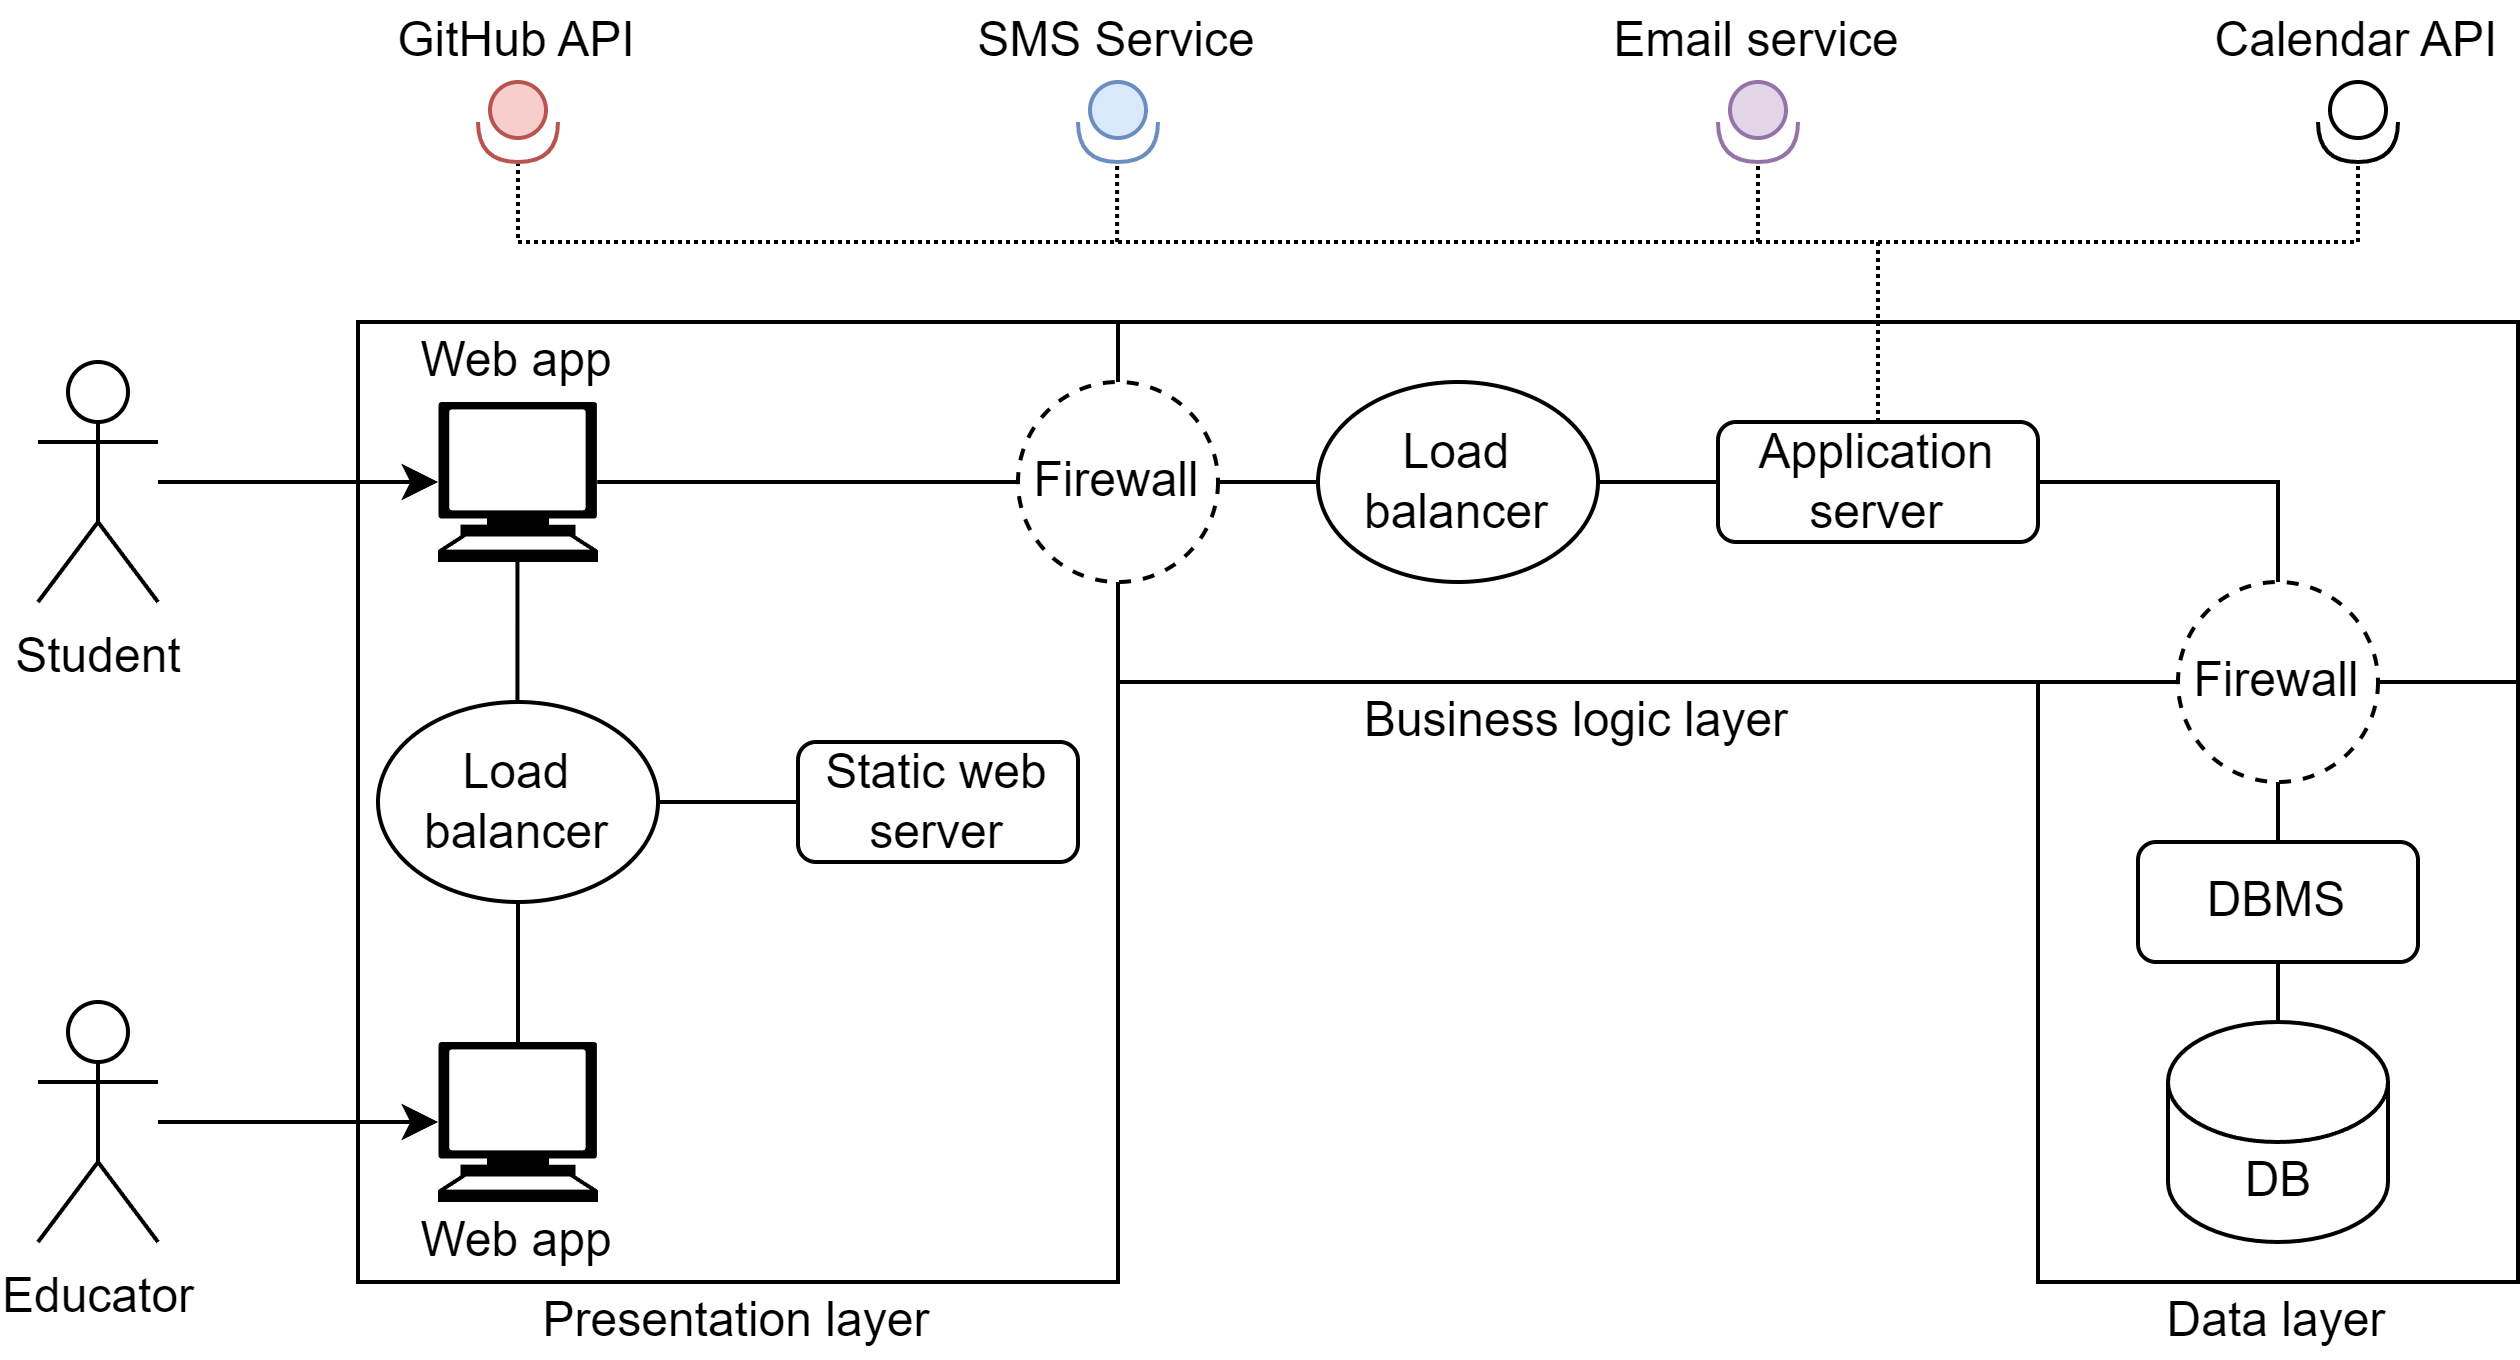
\includegraphics[width=0.9\linewidth]{images/high_level_architecture.png}
    \end{figure}
    The service will be accessed through a web interface, utilizing a single page application (SPA) that proves advantageous for this application type, enabling extensive interaction without frequent page reloads, thereby ensuring a faster and smoother user experience. 
    The system's architecture is structured three into distinct layers, with application servers interacting with a database management system and utilizing APIs for data retrieval and storage. 
    Adhering to REST standards, the application servers are designed to be stateless, and the system incorporates firewalls to bolster security.
    
    \section{Component view}
    \begin{figure}[H]
        \centering
        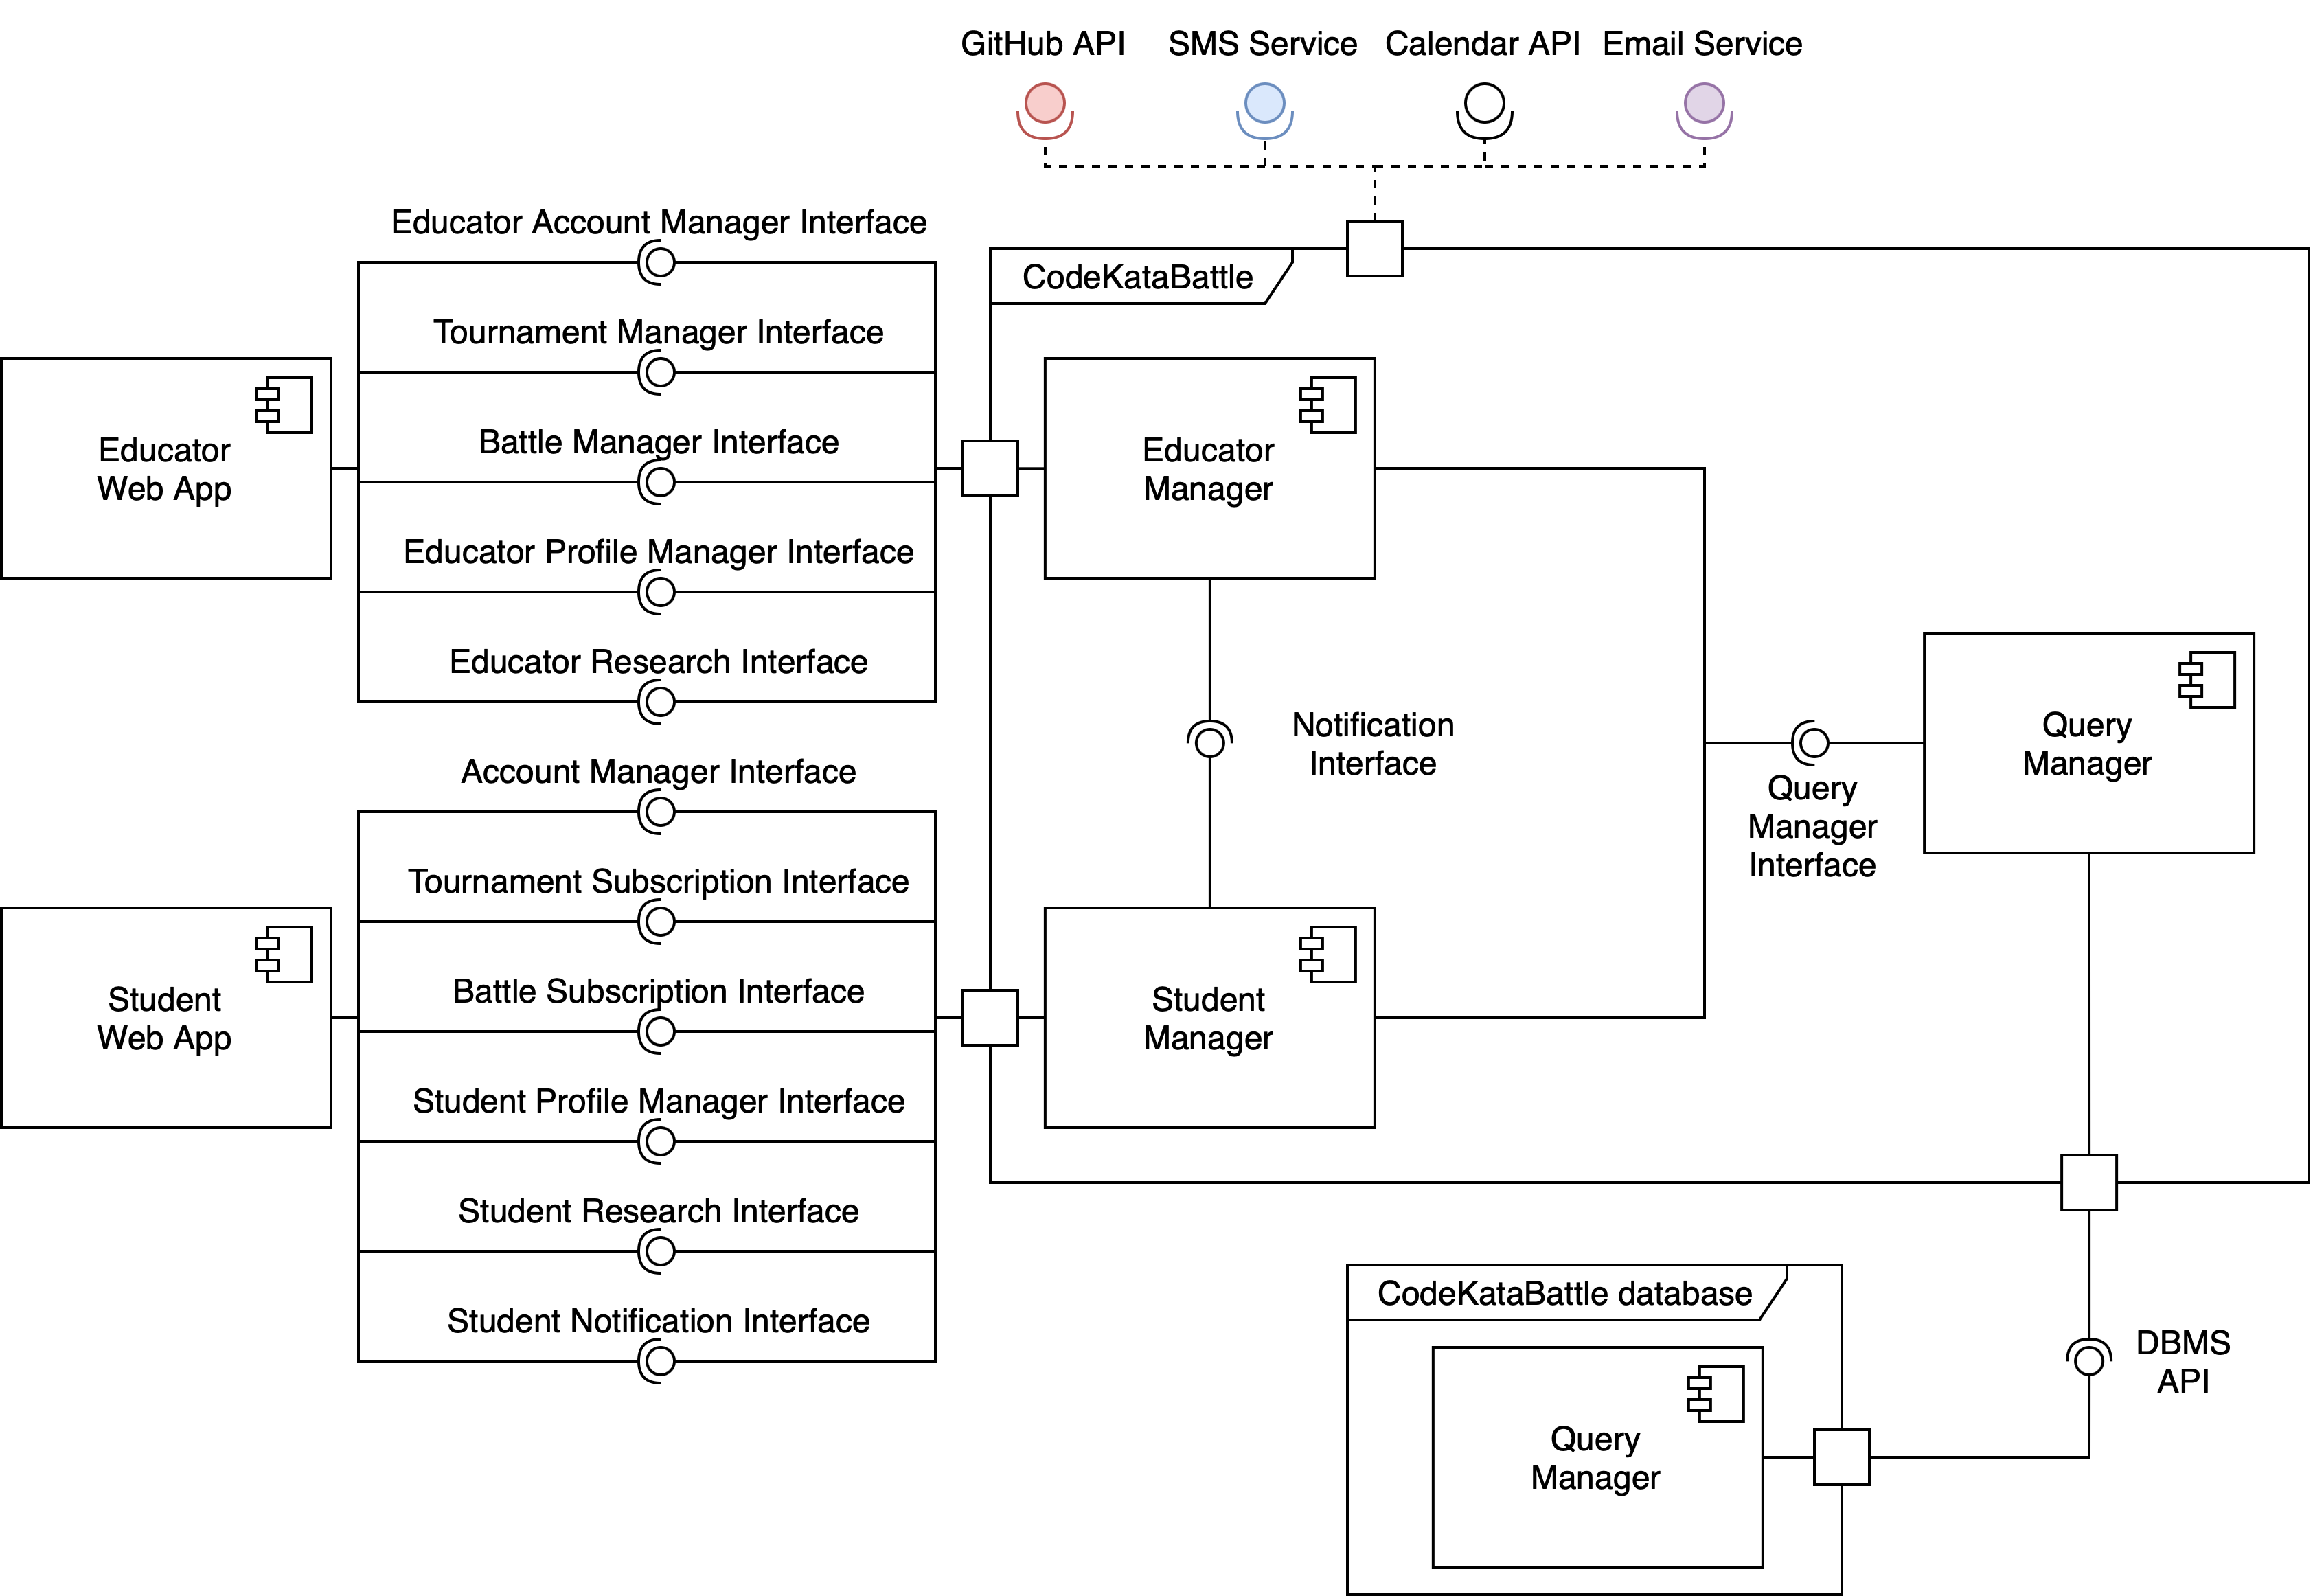
\includegraphics[width=1\linewidth]{images/component_view.png}
        \caption{Component diagram of the CodeKataBattle system}
    \end{figure}
    The component diagram contains all the interfaces used by the educators and the students. 
    These components will be better explained and analyzed in the following pages. 
    Both components have an interface with the database, that deals with the data of all the system. 
    The system has also access to some external API that are inserted at the top of the diagram.  

    \subsection{Query manager}
    This element is tasked with interfacing with a Database Management System (DBMS). 
    It adheres to the Adapter design pattern, enabling seamless interaction between other components and the DBMS without necessitating the manual writing of SQL code.

    \subsection{Educator manager}
    The educator manager component is responsible for interacting with educators.
    It allows the educator to log in, register, manage the profile, search for a tournament, create a tournament, create a battle, check the leaderboards, manage a tournament and give points to the students. 
    \begin{figure}[H]
        \centering
        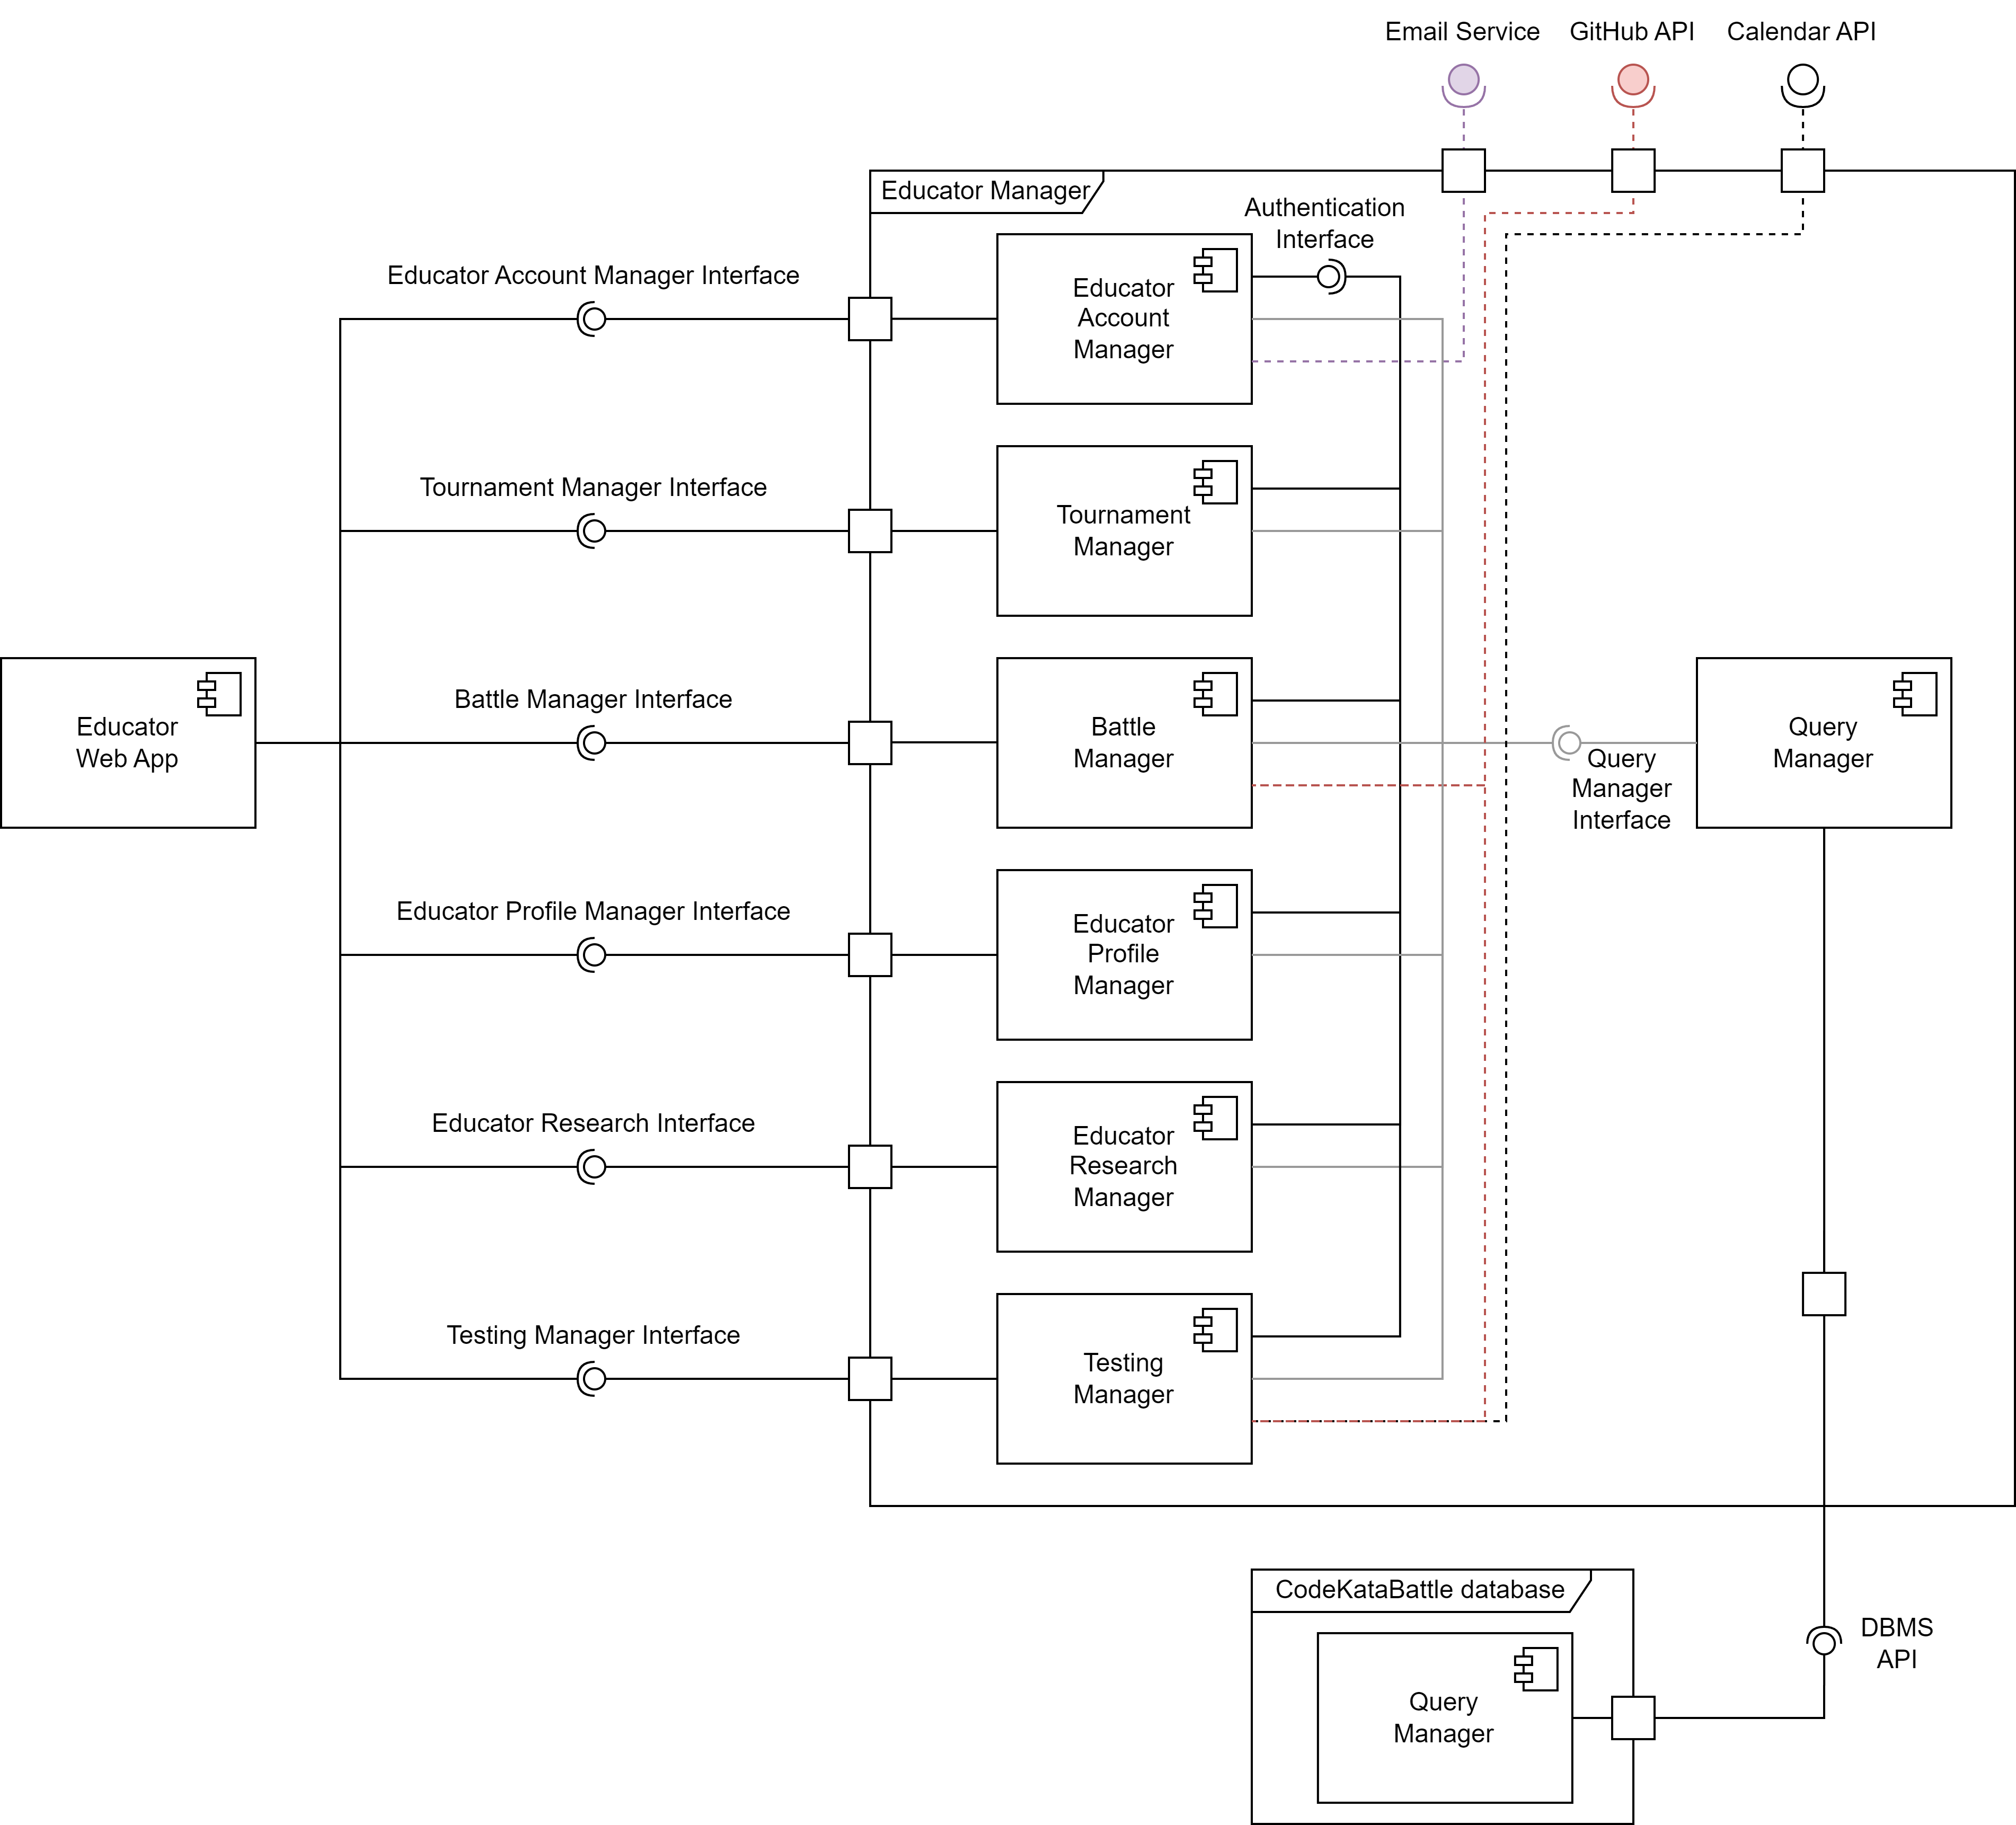
\includegraphics[width=0.8\linewidth]{images/component_view_educator.png}
    \end{figure}
    The educator manager component is expandend in five component as follows: 
    \begin{itemize}
        \item \textit{Account Manager}: this component allows the educators to log in and register to the system.
            It has an authentication interfaces that allows all other components to check if the educator is logged in and is allowd to do certain actions. 
            The account manager is also linked to the database through the query manager interface, that allows it to manage data in the tables dedicated to the educator.
            The only external API used by it is the email service that is utilized to verify the email whenever a new eduator tries to register. 
        \item \textit{Tournament Manager}: this component allows the educators to manage a tournament with the following actions: create a tournament, add a collaborator to a tournament, and close a tournament. 
            It has a connection to the authentication manager since it needs to verify the user that is tring to modify the tournament. 
            The tournament manager is also linked to the database through the query manager interface, that allows it to gather and add data to the tables dedicated to the tournament.
            The only external API used by it is the calendar API that is utilized to check the current date and the closure date of the tournament.
        \item \textit{Battle Manager}: this component allows the educators to manage a battle with the following actions: create a battle in a managed tournament, give personal evaluation (that modifies the gruop point), and close a battle. 
            It has a connection to the authentication manager since it needs to verify the user that is tring to modify the battle. 
            The battle manager is also linked to the database through the query manager interface, that allows it to gather and add data to the tables dedicated to the battle.
            The external APIs used by this component are: GitHub API to create the repository linked to the battle, SMS service to notify the user on the event of the newly created battle, and calendar API to check the main deadlines and notify the educators that manage the battle.
        \item \textit{Profile Manager}: this component allows the educators to check the personal profile with personal information and tournaments information. 
            It has an authentication interfaces that allows all other components to check if the educator is logged in and is allowed to check the desired profile. 
            The profile manager is also linked to the database through the query manager interface, that allows it to manage data in the tables dedicated to the educator's profile.
        \item \textit{Research Manager}: this component allows the educators to search all the active tournament in the system and to check all the leaderboards and rankings. 
            It has an authentication interfaces that allows all other components to check if the educator is logged in.
            The research manager is also linked to the database through the query manager interface, that allows it to manage data in the tables dedicated to the tournaments.
    \end{itemize}

    \subsection{Student manager}
    The student manager component is responsible for interacting with students.
    It allows the student to log in, register, manage the profile, search for a tournament, join a tournament, join a battle, and check the leaderboards.  
    \begin{figure}[H]
        \centering
        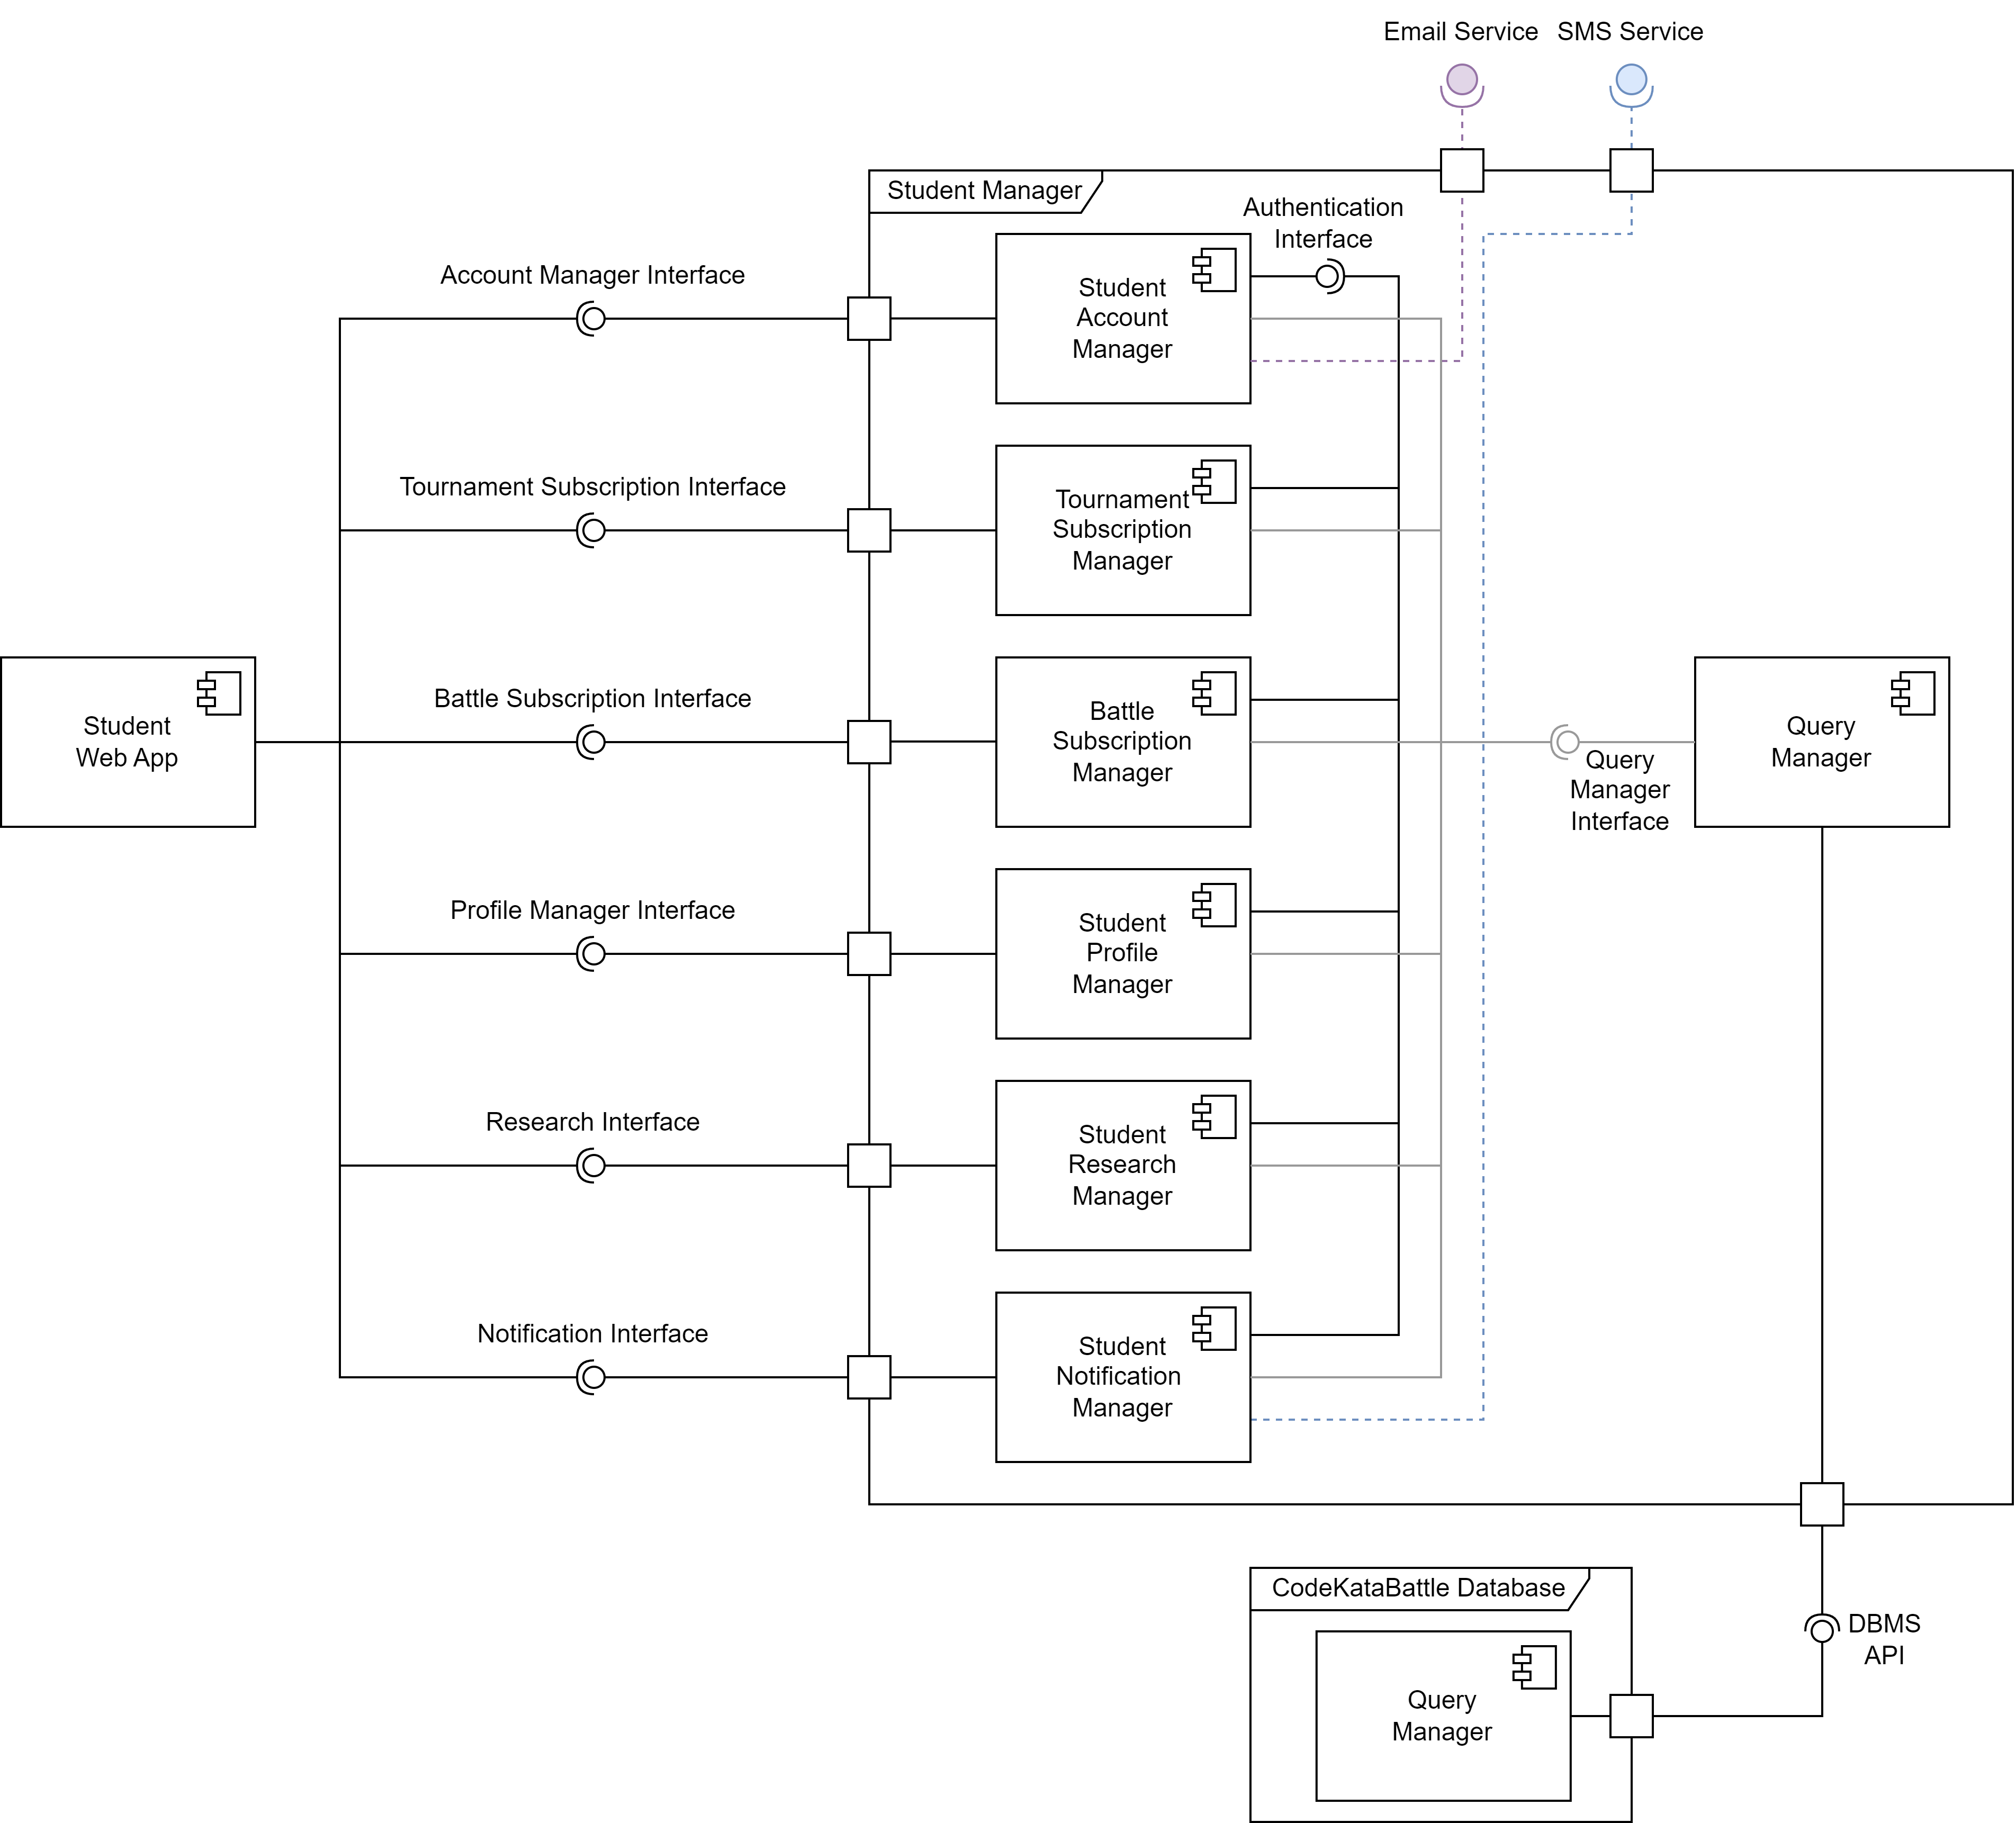
\includegraphics[width=0.8\linewidth]{images/component_view_student.png}
    \end{figure}
    The student manager component is expandend in five component as follows: 
    \begin{itemize}
        \item \textit{Account Manager}: this component allows the students to log in and register to the system.
            It has an authentication interfaces that allows all other components to check if the student is logged in and is allowed to do certain actions. 
            The account manager is also linked to the database through the query manager interface, that allows it to manage data in the tables dedicated to the student.
            The only external API used by it is the email service that is utilized to verify the email whenever a new student tries to register. 
        \item \textit{Tournament Subscription Manager}: this component allows the students to enroll in a tournament with the following actions.
            It has a connection to the authentication manager since it needs to verify the user that is tring to enroill in a tournament. 
            The tournament subscription manager is also linked to the database through the query manager interface, that allows to register the student to the tournament. 
            The external APIs used by this component are: SMS service to notify the user on the event of the tournament, and calendar API to check the main deadlines and notify the students that are enrolled in the tournament.
        \item \textit{Battle Subscription Manager}: this component allows the students to enroll in a battle within a tournament where they are already subscribed. 
            It has a connection to the authentication manager since it needs to verify the user that is tring to enroll in the battle. 
            The battle subscription manager is also linked to the database through the query manager interface, that allows it to gather and add data to the tables dedicated to the battle.
            The external APIs used by this component are the SMS service to notify the user on the event of the newly created battle, and the calendar API to check the main deadlines and notify the students that are enrolled in the battle.
        \item \textit{Profile Manager}: this component allows the students to check the personal profile with personal information and enrolled tournaments information. 
            It has an authentication interfaces that allows all other components to check if the student is logged in and is allowed to check the desired profile. 
            The profile manager is also linked to the database through the query manager interface, that allows it to manage data in the tables dedicated to the student's profile.
        \item \textit{Research Manager}: this component allows the students to search all the active tournament in the system and to check all the leaderboards and rankings. 
            It has an authentication interfaces that allows all other components to check if the student is logged in.
            The research manager is also linked to the database through the query manager interface, that allows it to manage data in the tables dedicated to the tournaments.
    \end{itemize}

    \newpage
    \subsection{Database schema}
    In this section there is the E-R schema used for the database of the system. 
    \begin{figure}[H]
        \centering
        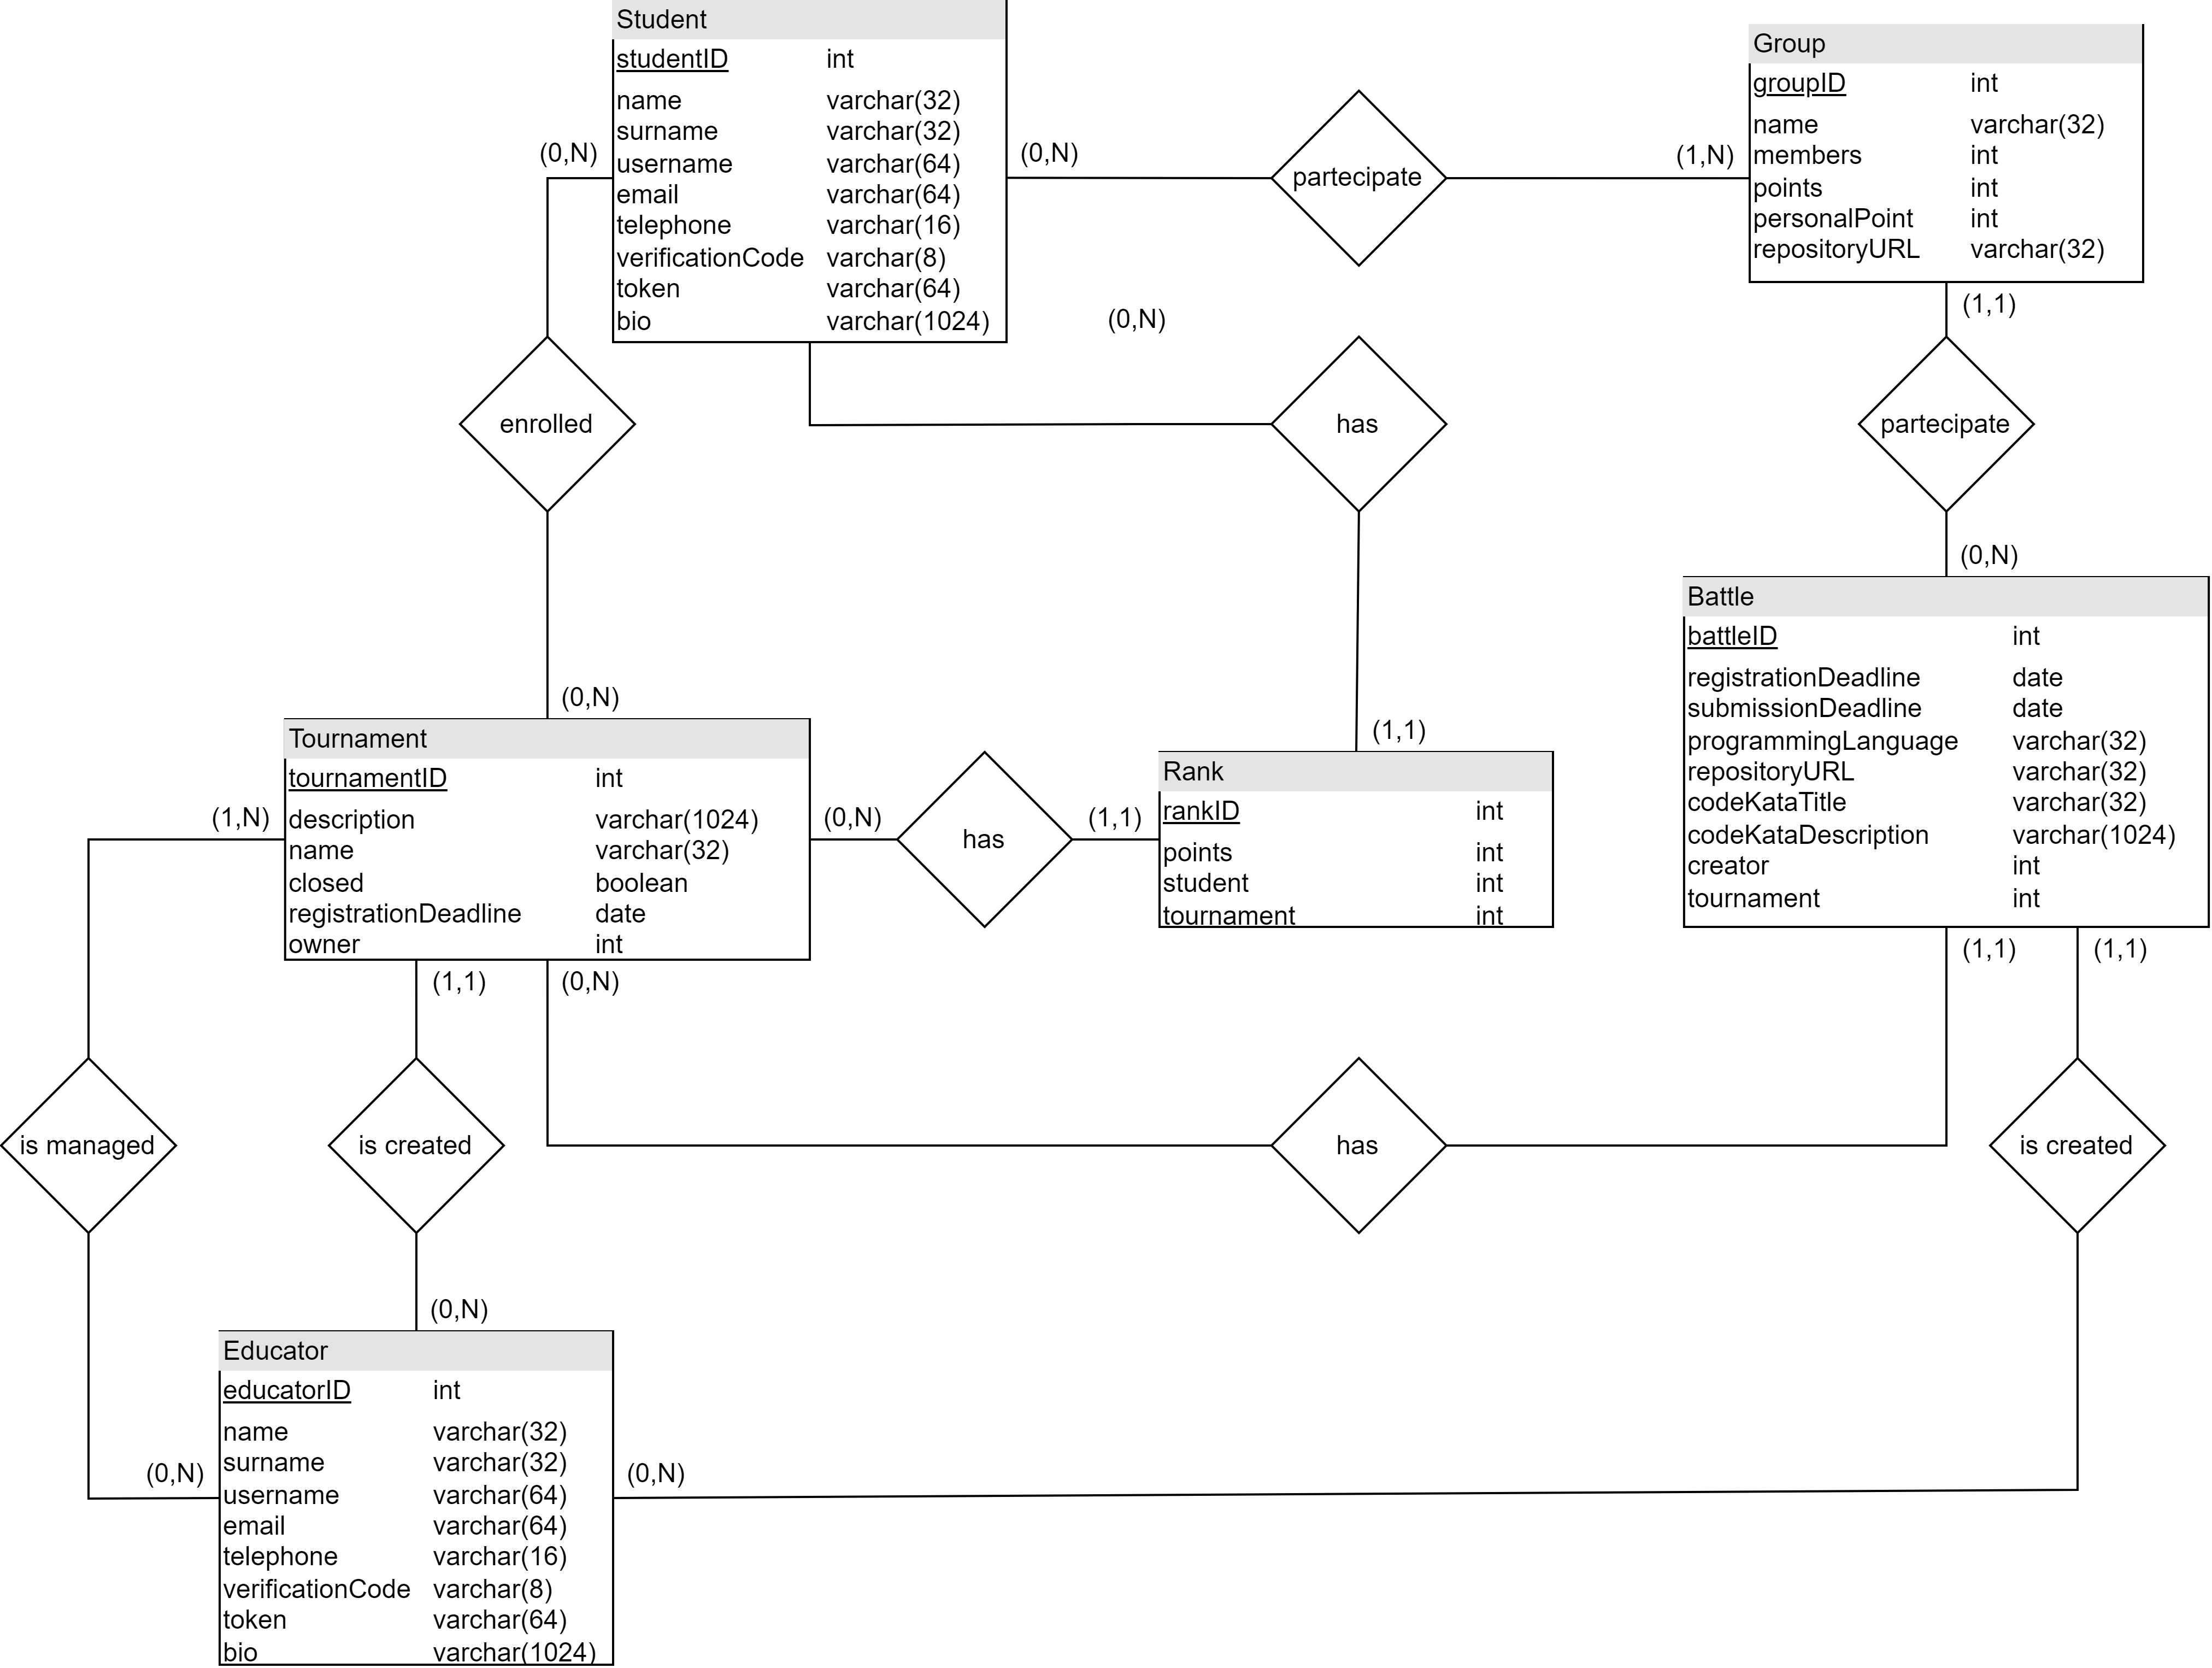
\includegraphics[width=0.9\linewidth]{images/db.png}
    \end{figure}
    Students and educators are stored in different tables to have better performance when searching the user in the database.
    The attributes of both tables are the same, and comprises: name, surname, username, email, and telephone. 
    Each student and educator has a unique numerical ID (it is possible to use also the username since we have the uniqueness constraint on it). 

    Group is a table that contains all the groups linked to all the existing battles. 
    It has the following attributes: name, members (the number of memmbers in the considered group), points (of the group in a battle), and repositoryURL (a string with the URL of the group repository for a battle).
    The ID is unique over all possible groups in all possible battles.
    
    Battle represents a single battle with the description of the problem associated with it. 
    The attributes are: registrationDeadline, submissionDeadline, programmingLanguage, repositoryURL (of the general repository to be forked), codeKataTitle, CodeKataDescription, creator (that is the ID of the educator that created the battle), and tournament (that is the ID of the tournament where the battle were created). 
    The ID is unique in the whole system. 

    Tournament represents the list of tournament that have ended (closed set to one) or are running (closed set to zero). 
    Other attributes are: description, name, registrationDeadline, and owner (that is the ID of the educator that created the tournament initially). 
    Also in this case we have a unique ID as key. 

    Rank contains the point associated to a student (ID of the student) for a certain tournament where he is enrolled (tournament is the ID of the linked tournament). 
    Each rank has a single ID. 


    \section{Deployment view}
    Our setup comprises two essential components: a static web server serving as the entry point for clients to access the Single Page Application (SPA), and an application server providing the requisite APIs for the SPA's functionality. 
    To optimize performance and leverage distinct advantages, we've adopted distinct solutions for each part.
    The static web server is deployed on a Content Delivery Network (CDN) to ensure rapid response times. 
    This is achieved through the utilization of edge location caches and reverse proxies. 
    On the other hand, the application server, encompassing both a business logic layer and a data tier, is hosted on a cloud provider. 
    This choice offers several benefits over conventional in-house hosting:
    \begin{itemize}
        \item \textit{Scalability and flexibility}: the cloud infrastructure allows us to dynamically adjust resources such as virtual machines, performance cores, or memory based on demand. Incorporating load balancing services enables the application server to seamlessly adapt to fluctuations in traffic or workload.
        \item \textit{Security}: leveraging services like live monitoring and firewalls enhances the security posture of the application server, safeguarding it against data breaches, cyberattacks, and other security threats.
        \item \textit{Cost-efficiency}: the cloud provider's pay-as-you-go model ensures cost optimization by billing only for the actual resources consumed. This approach proves economical and contributes to lowering overall operational expenses.
    \end{itemize}
    These features collectively position a cloud provider as an optimal choice for hosting large, high-traffic applications. 
    It is imperative that the chosen cloud provider offers comprehensive support for scalability, security, and cost-efficiency to align with our specific requirements.
    \begin{figure}[H]
        \centering
        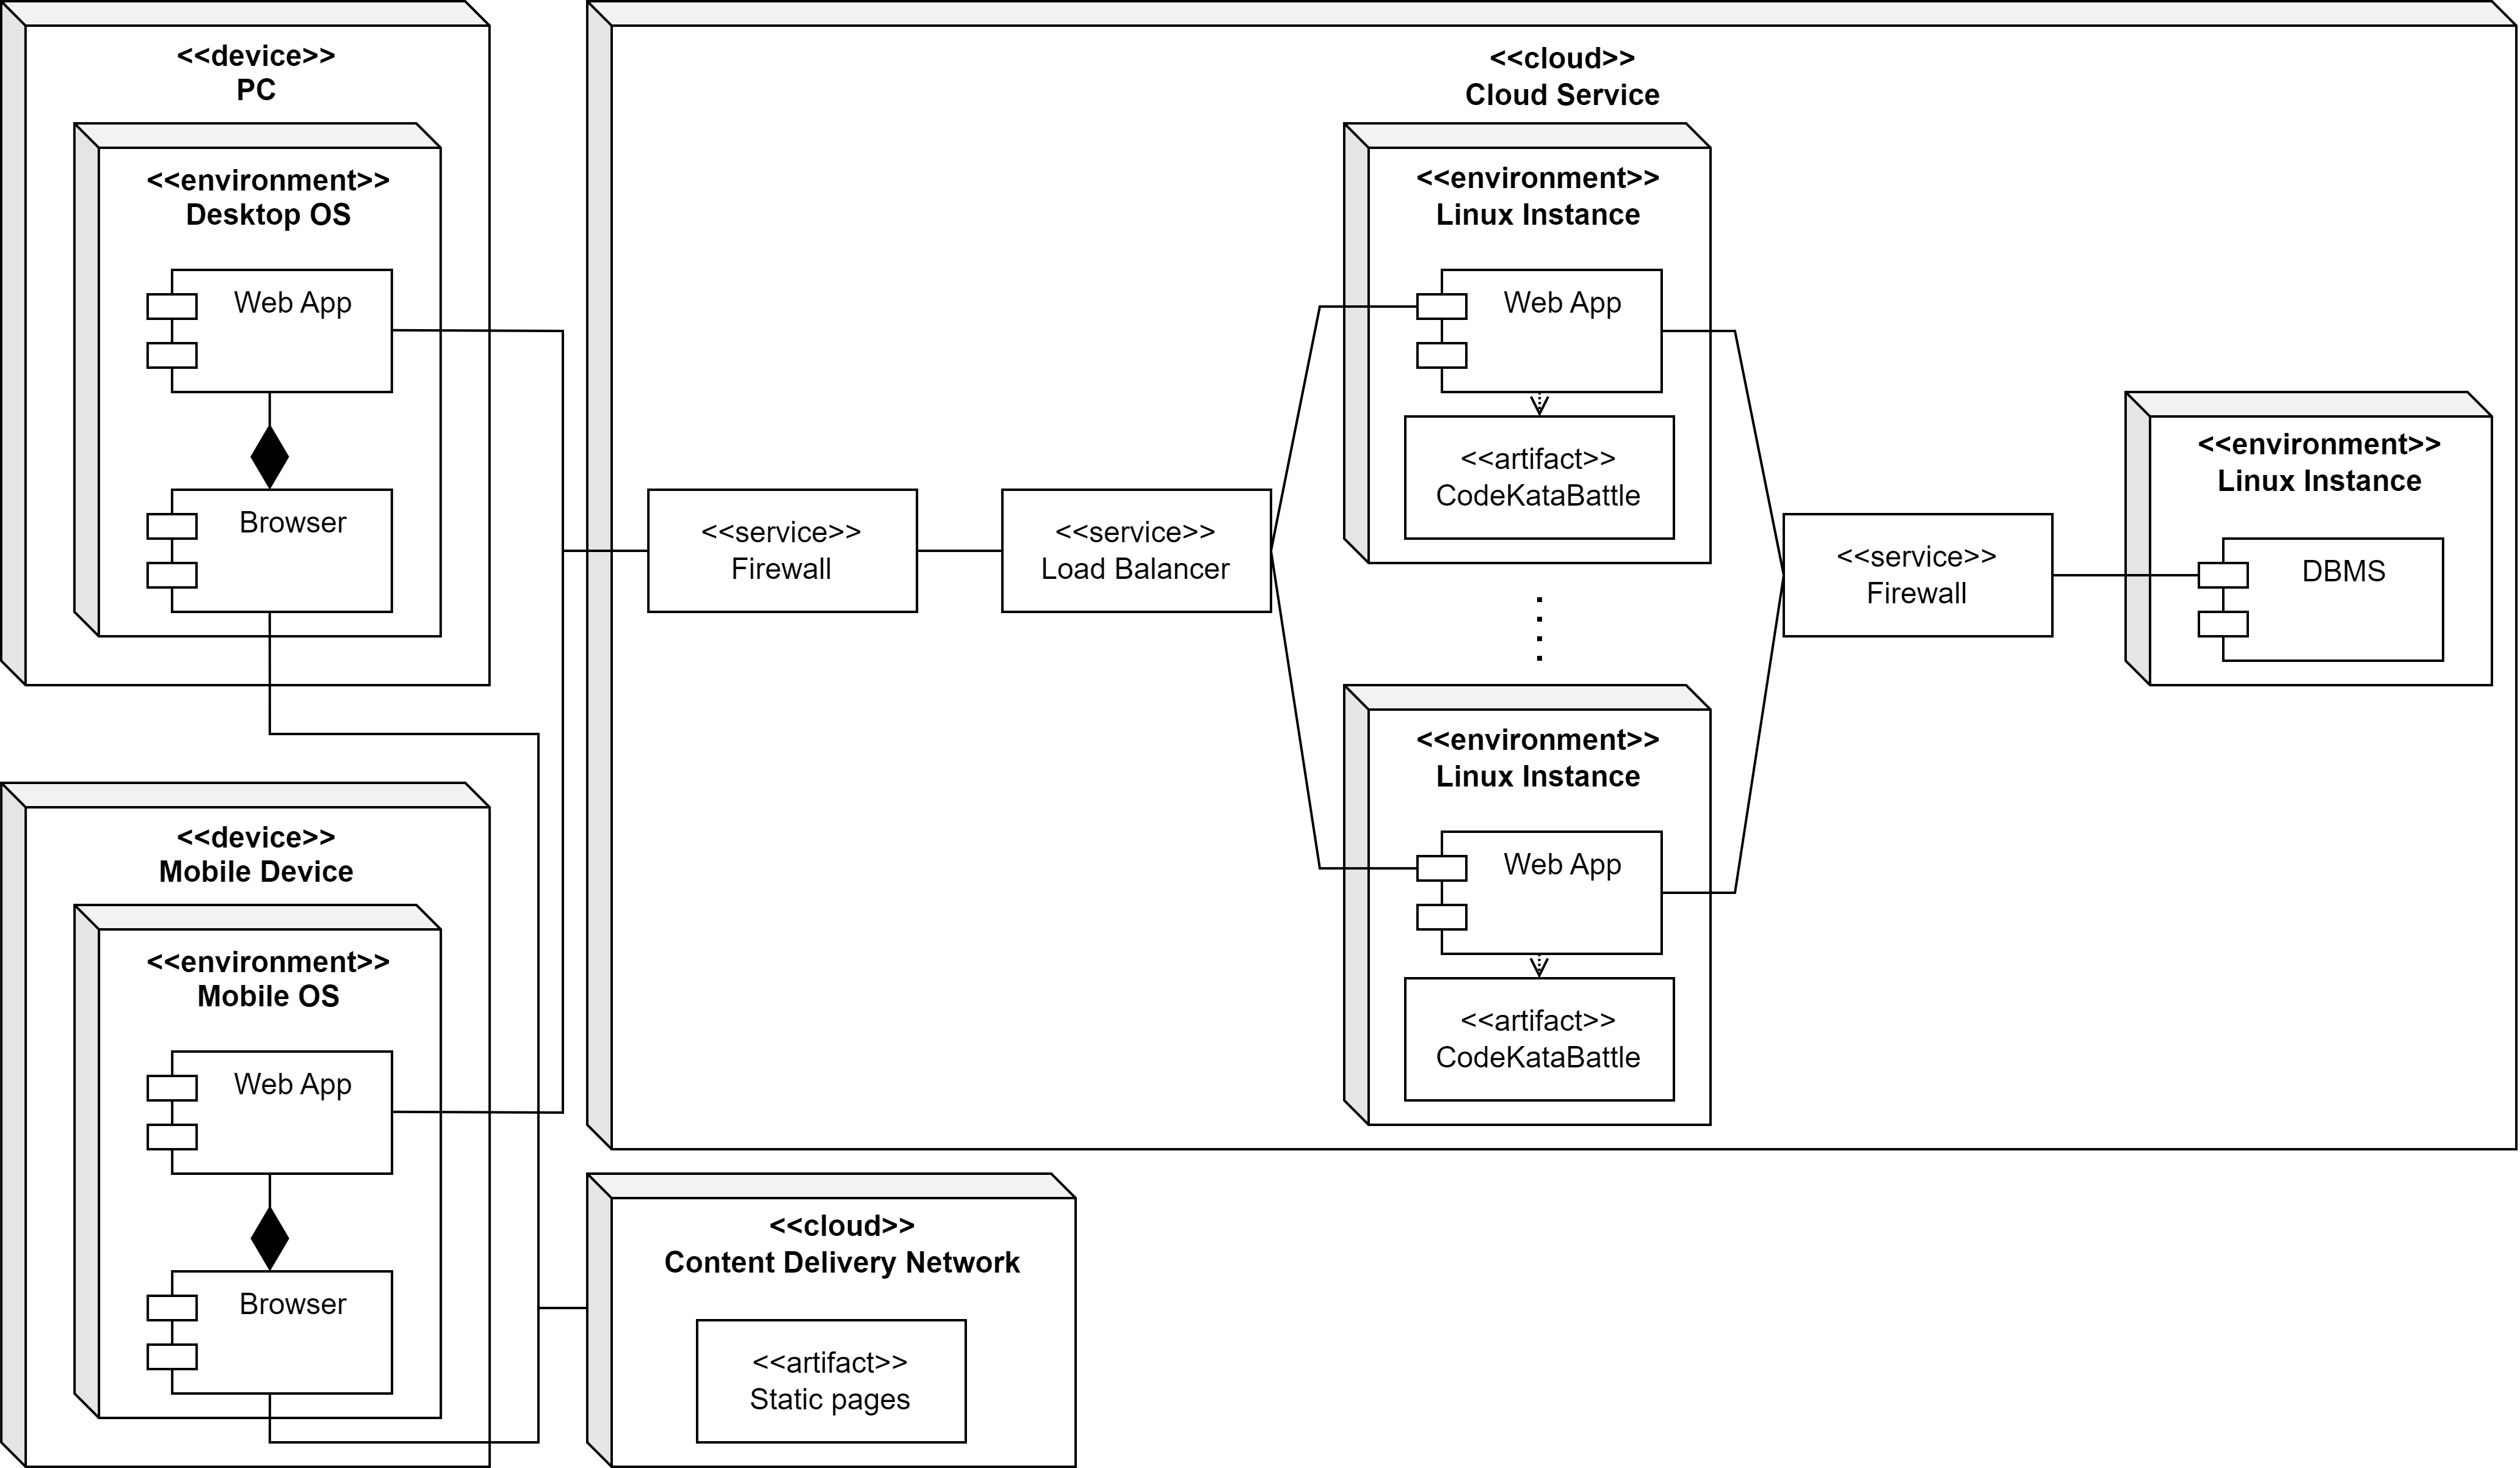
\includegraphics[width=0.9\linewidth]{images/deployment_view.png}
        \caption{Deployment views}
    \end{figure}
    The devices called PC and Mobile are any device with a moder browser capable of running JavaScript. 
    
    The static pages are handled by the Content Delivery Network to avoid affecting the performance of the main application. 
    This part handles the welcome page and login/register pages. 
    These pages are static in the sense that they have no need to have code that runs on server side. 

    Finally, the cloud service will host all the business and data logic. 
    This service contains the following elements: 
    \begin{itemize}
        \item \textit{Firewall services}: employed to filter incoming connections to both the business and data layers of a system, firewall services utilize a predetermined set of rules selected based on specific criteria. 
            This component serves as a crucial defense mechanism against malicious attacks, offering generic filtering capabilities.
        \item \textit{Load balancer}: tasked with distributing incoming traffic among multiple instances of an application, the load balancer serves to optimize resource utilization, enhance performance, and ensure high availability. 
            Its role is critical in preventing application overload or downtime, and it contributes to a stable and reliable user experience by redirecting traffic to the least busy application instance.
        \item \textit{Multiple application instances}: operating in parallel and independently, multiple copies of the application can be dynamically created or deleted to meet demand. 
            This approach enables the application to efficiently handle a high volume of requests without encountering performance issues. 
            Additionally, it provides fault tolerance by redirecting traffic to alternative instances in case one becomes unavailable.
        \item \textit{Data instance}: this component involves a data-optimized virtual machine housing the Database Management System (DBMS) and the associated database. 
            It plays a pivotal role in managing and organizing data efficiently within the system.
    \end{itemize}

    \section{Runtime view}
    \subsection{Student's runtime view}
    In this section we list all possible actions for the student along with the runtime view associated with each one. 
    
    \paragraph*{Student signup}
    In this case the actor is an unregistered student that is trying to sign up in the system.
    After accessing the corresponding page the student submits all the required information to the student account manager component that cheks the data. 
    If the user is not already register it creates a new student after the email verification. 
    \begin{figure}[H]
        \centering
        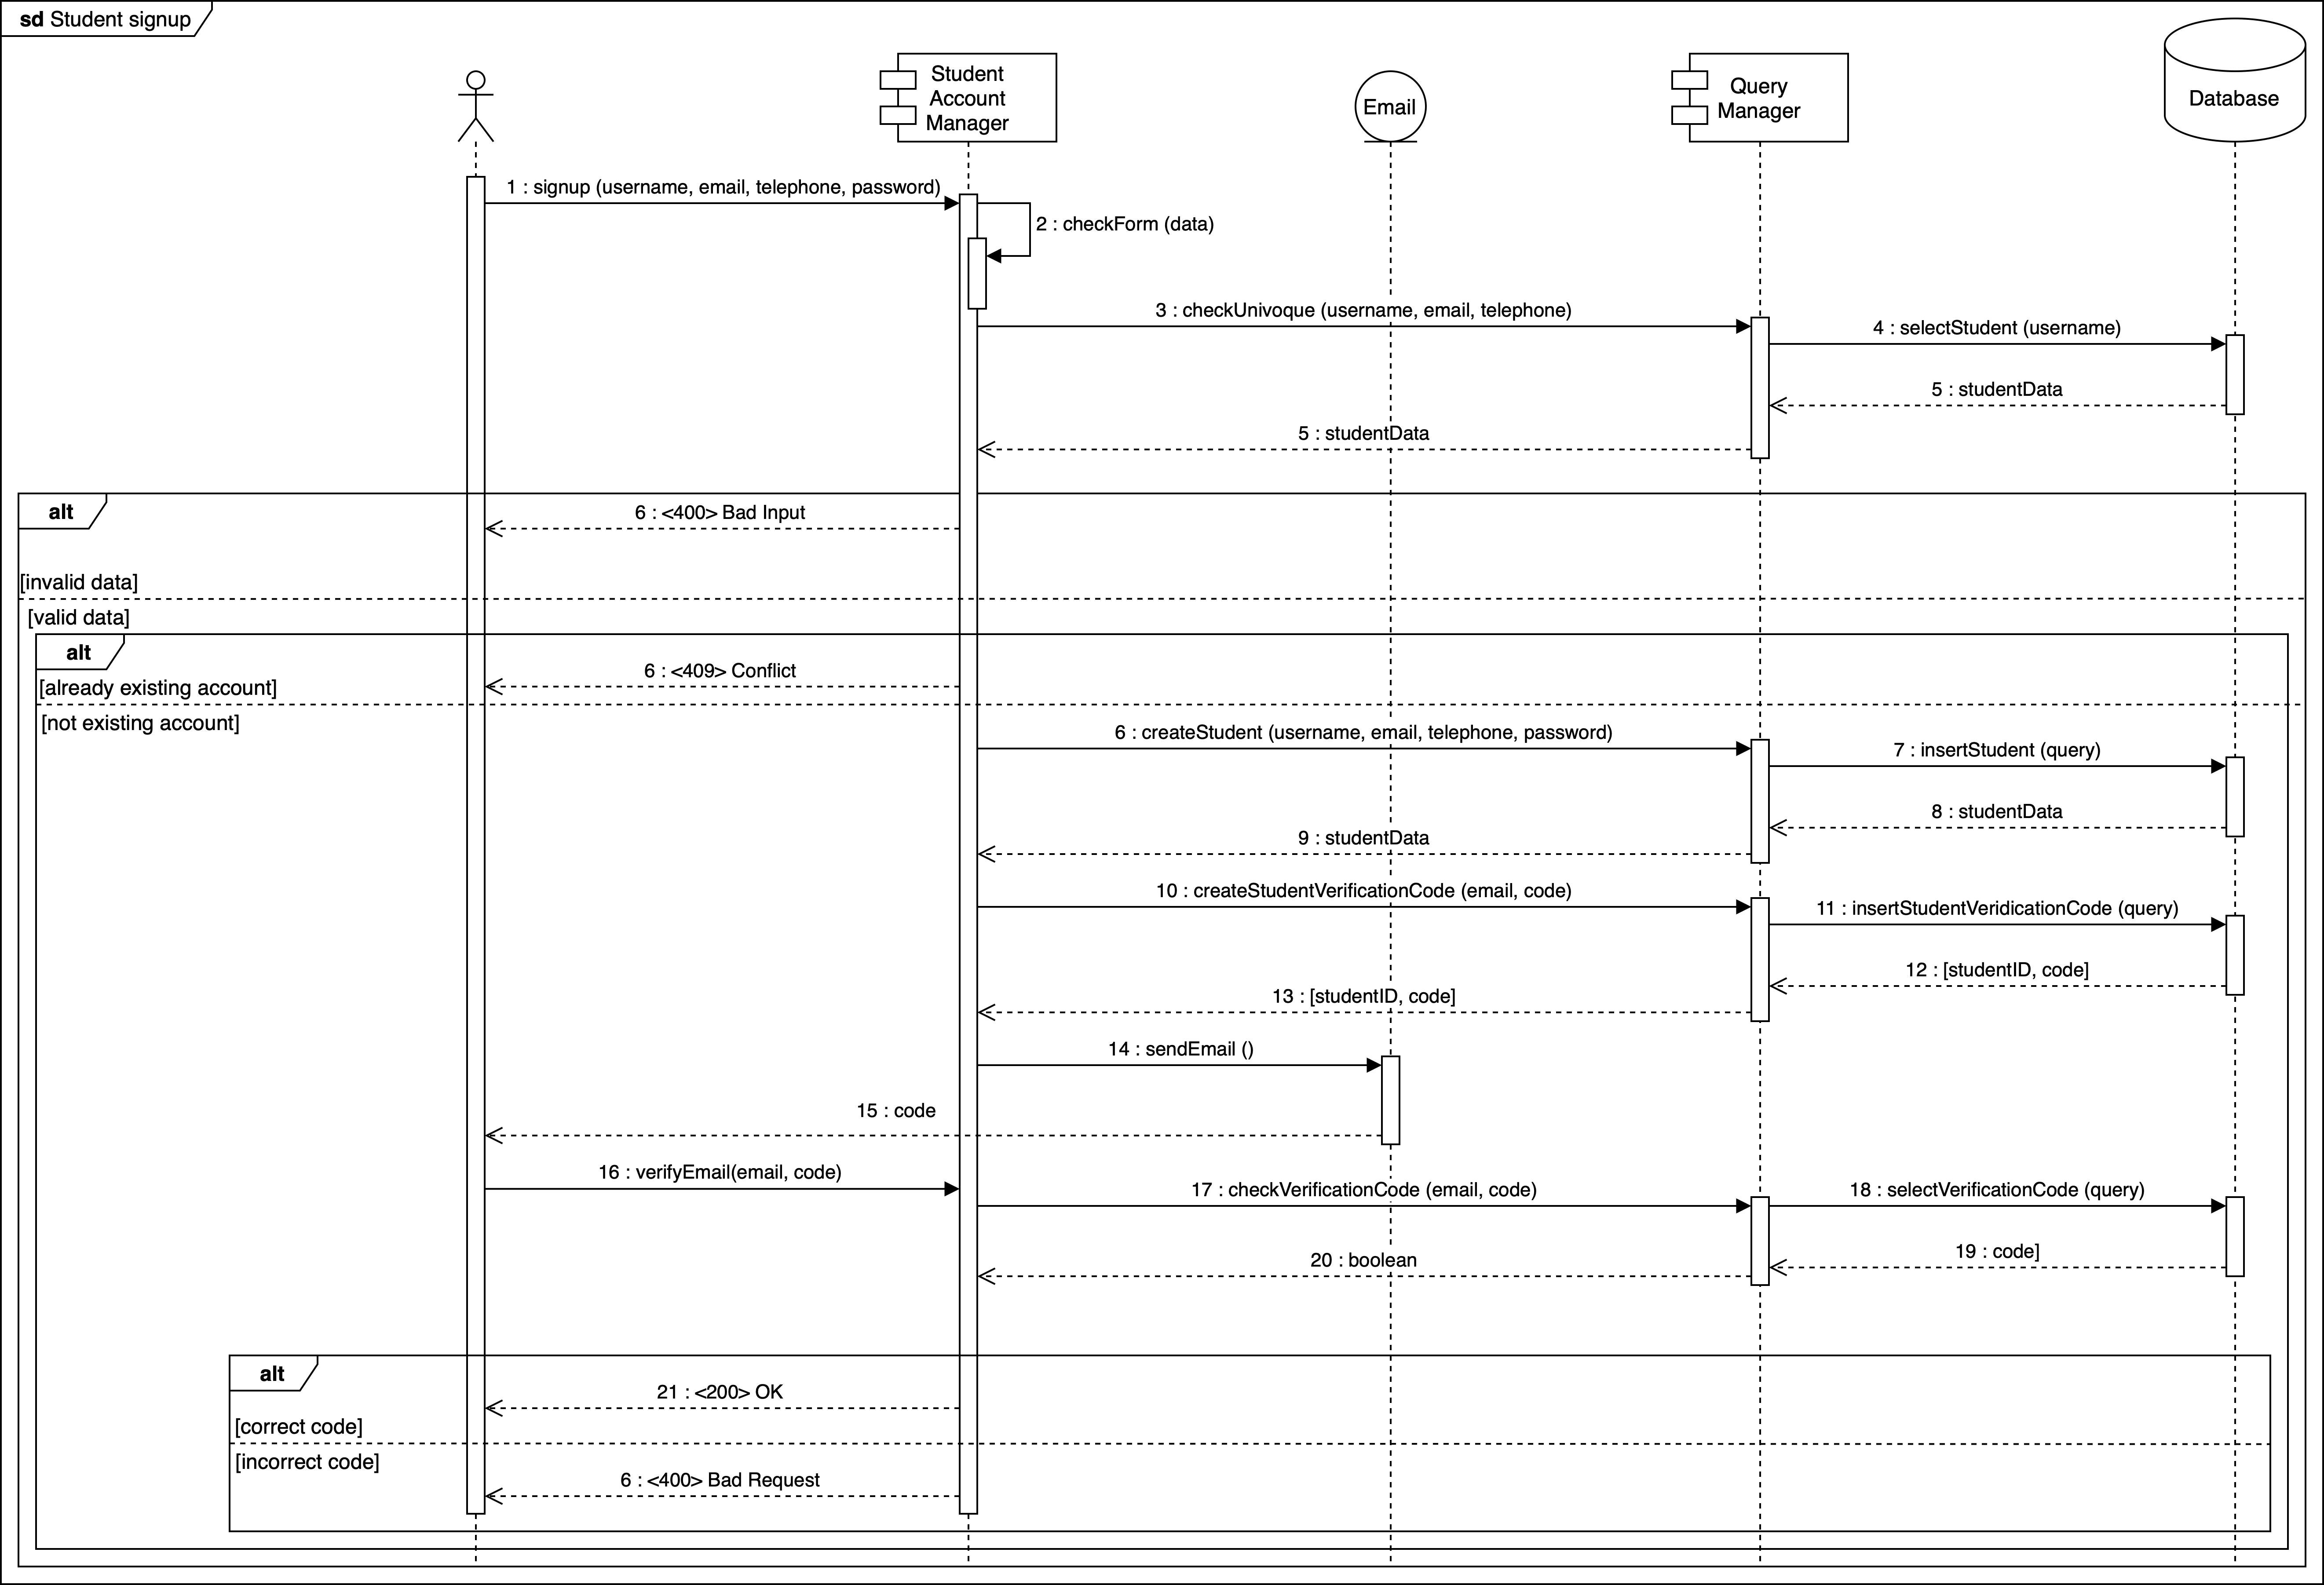
\includegraphics[width=1.0\linewidth]{images/ssrv.png}
    \end{figure}

    \paragraph*{Student log in}
    In this case the actor is a registered student that wants to log in into the system. 
    After accessing the corresponding page the student submits all the required information to the student account manager component that cheks the data. 
    If the inserted data are correct the student can access all his possible actions. 
    \begin{figure}[H]
        \centering
        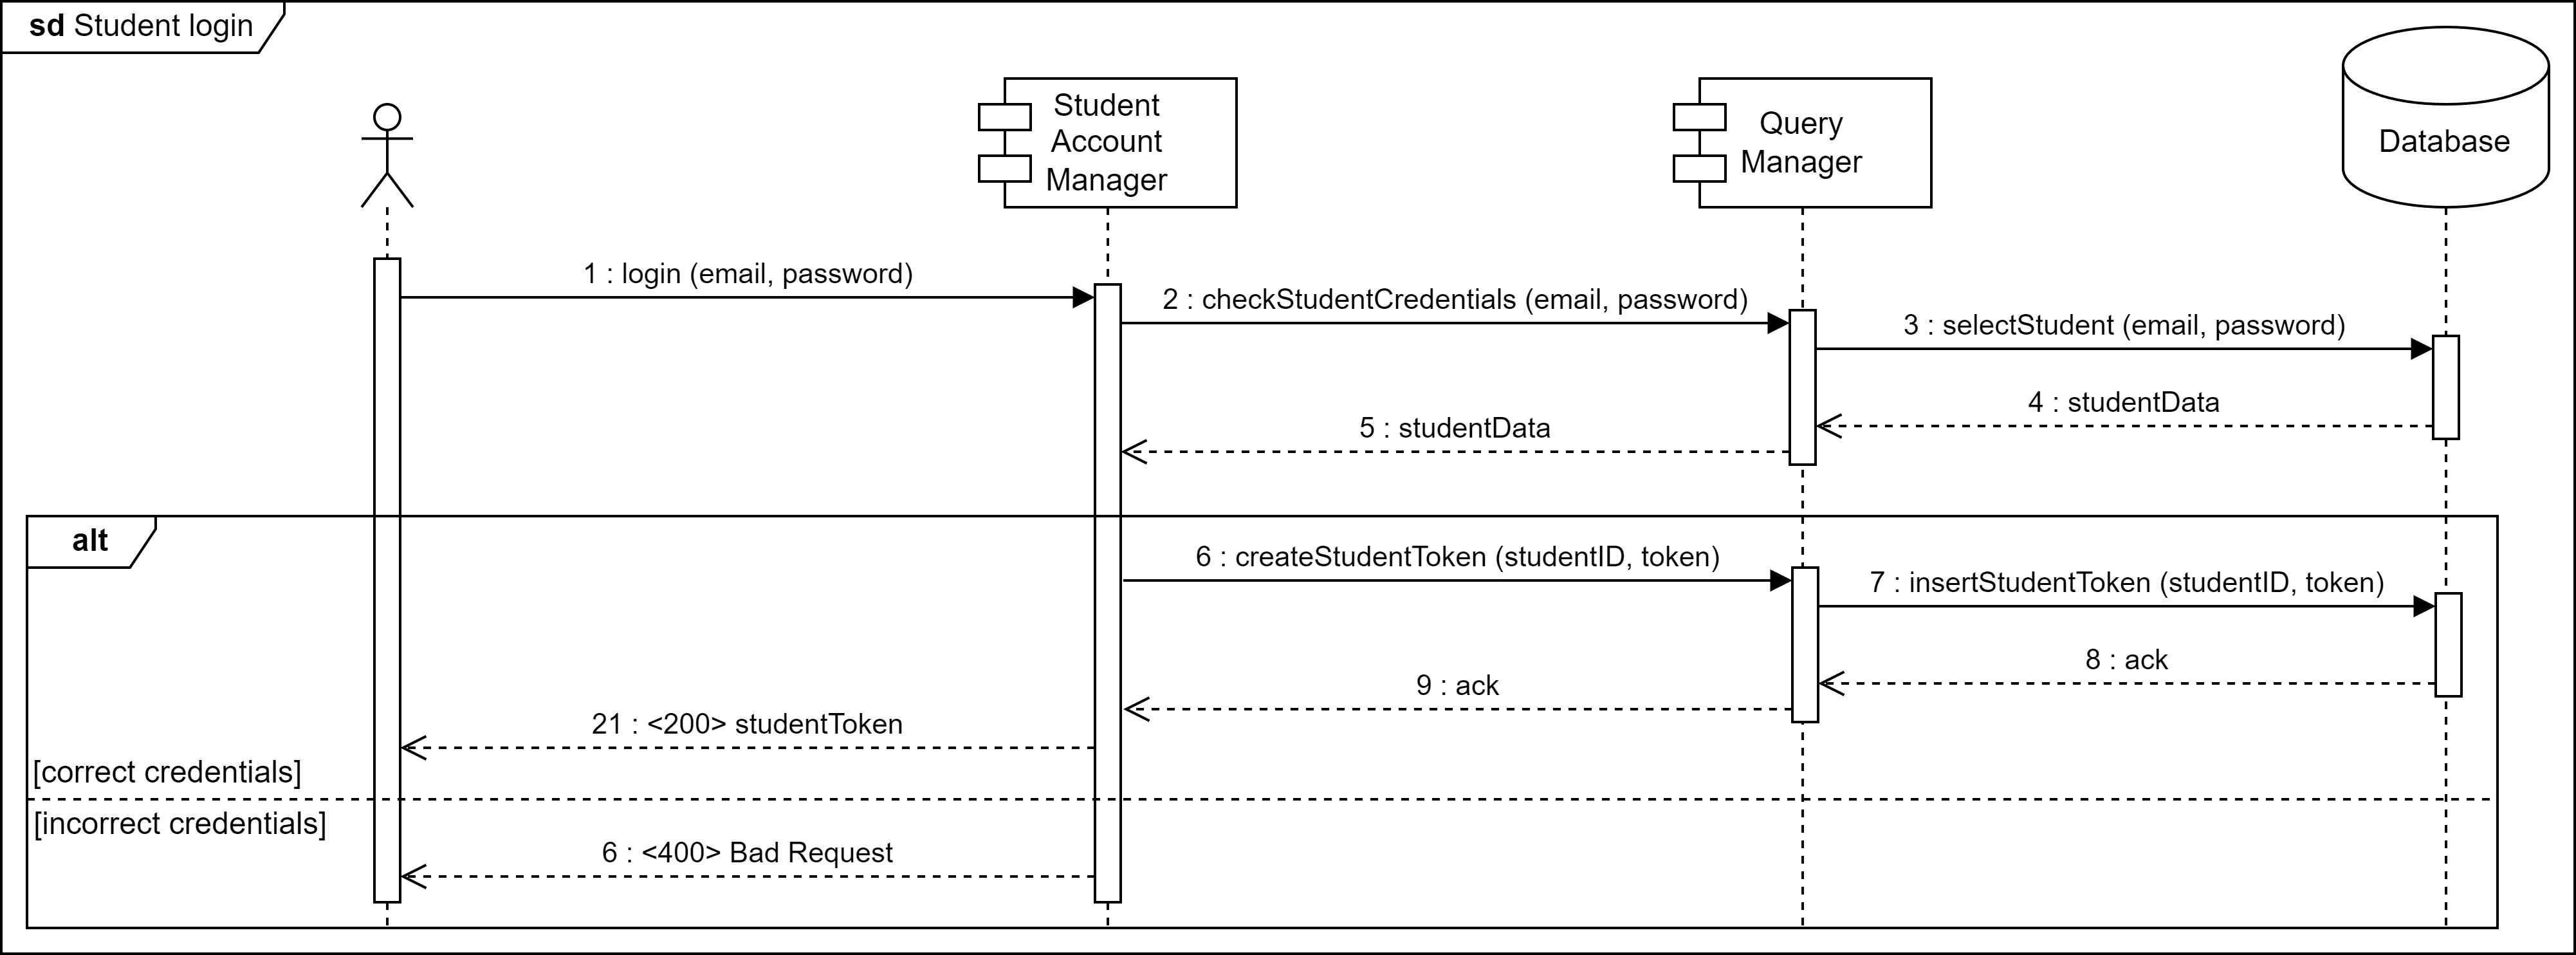
\includegraphics[width=1.0\linewidth]{images/slrv.png}
    \end{figure}

    \paragraph*{Student profile}
    In this case the actor is a registered student that wants to check his own profile. 
    The student profile manager retrieves all the data linked to the student and returns the complete page to the student. 
    \begin{figure}[H]
        \centering
        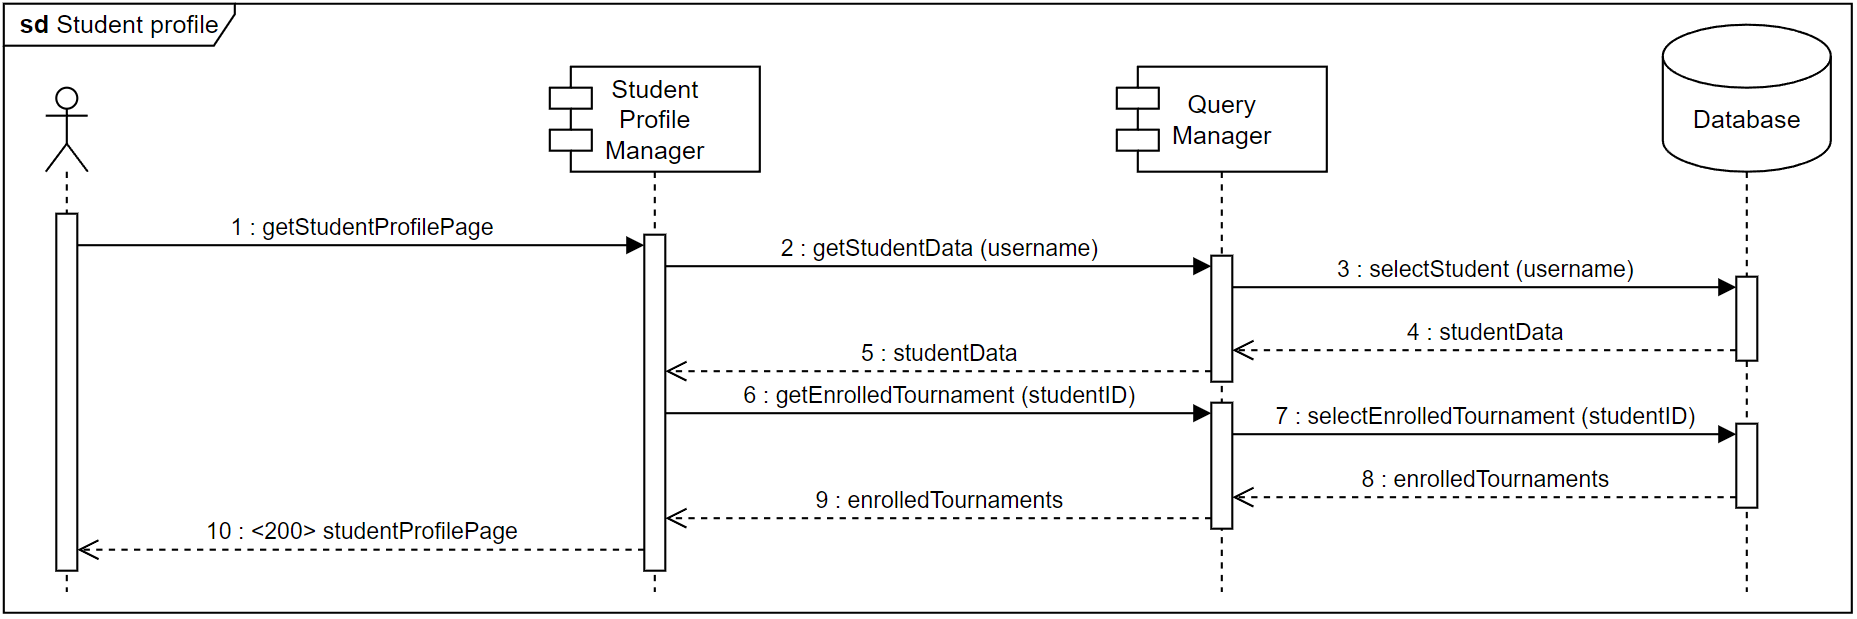
\includegraphics[width=1.0\linewidth]{images/sprv.png}
    \end{figure}

    \paragraph*{Student home page}
    In this case the actor is a registered student that wants to access the home page. 
    The student research manager retrieves all the active tournaments from the database and return the home page with some tournaments. 
    \begin{figure}[H]
        \centering
        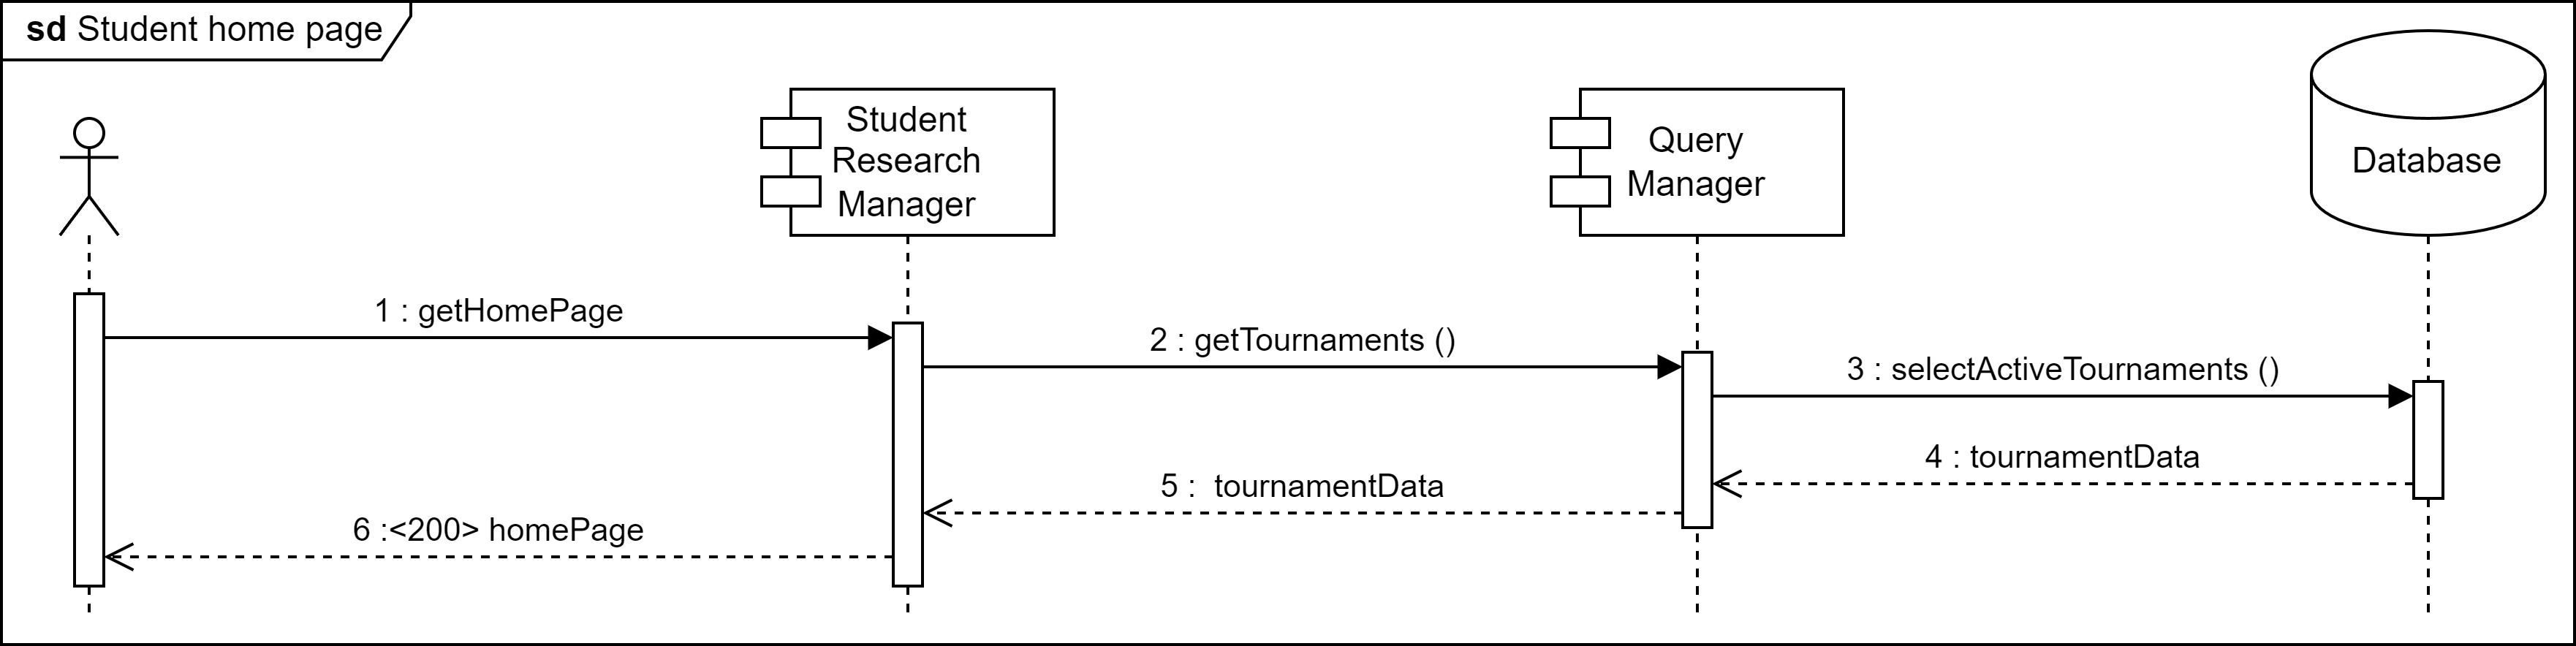
\includegraphics[width=1.0\linewidth]{images/shprv.png}
    \end{figure}

    \paragraph*{Student join tournament}
    In this case the actor is a registered student that wants to join a tournament. 
    The student requests the home page and then select the desired tournament. 
    After clicking the join button the system return the consequence of the action (enrolled or not). 
    \begin{figure}[H]
        \centering
        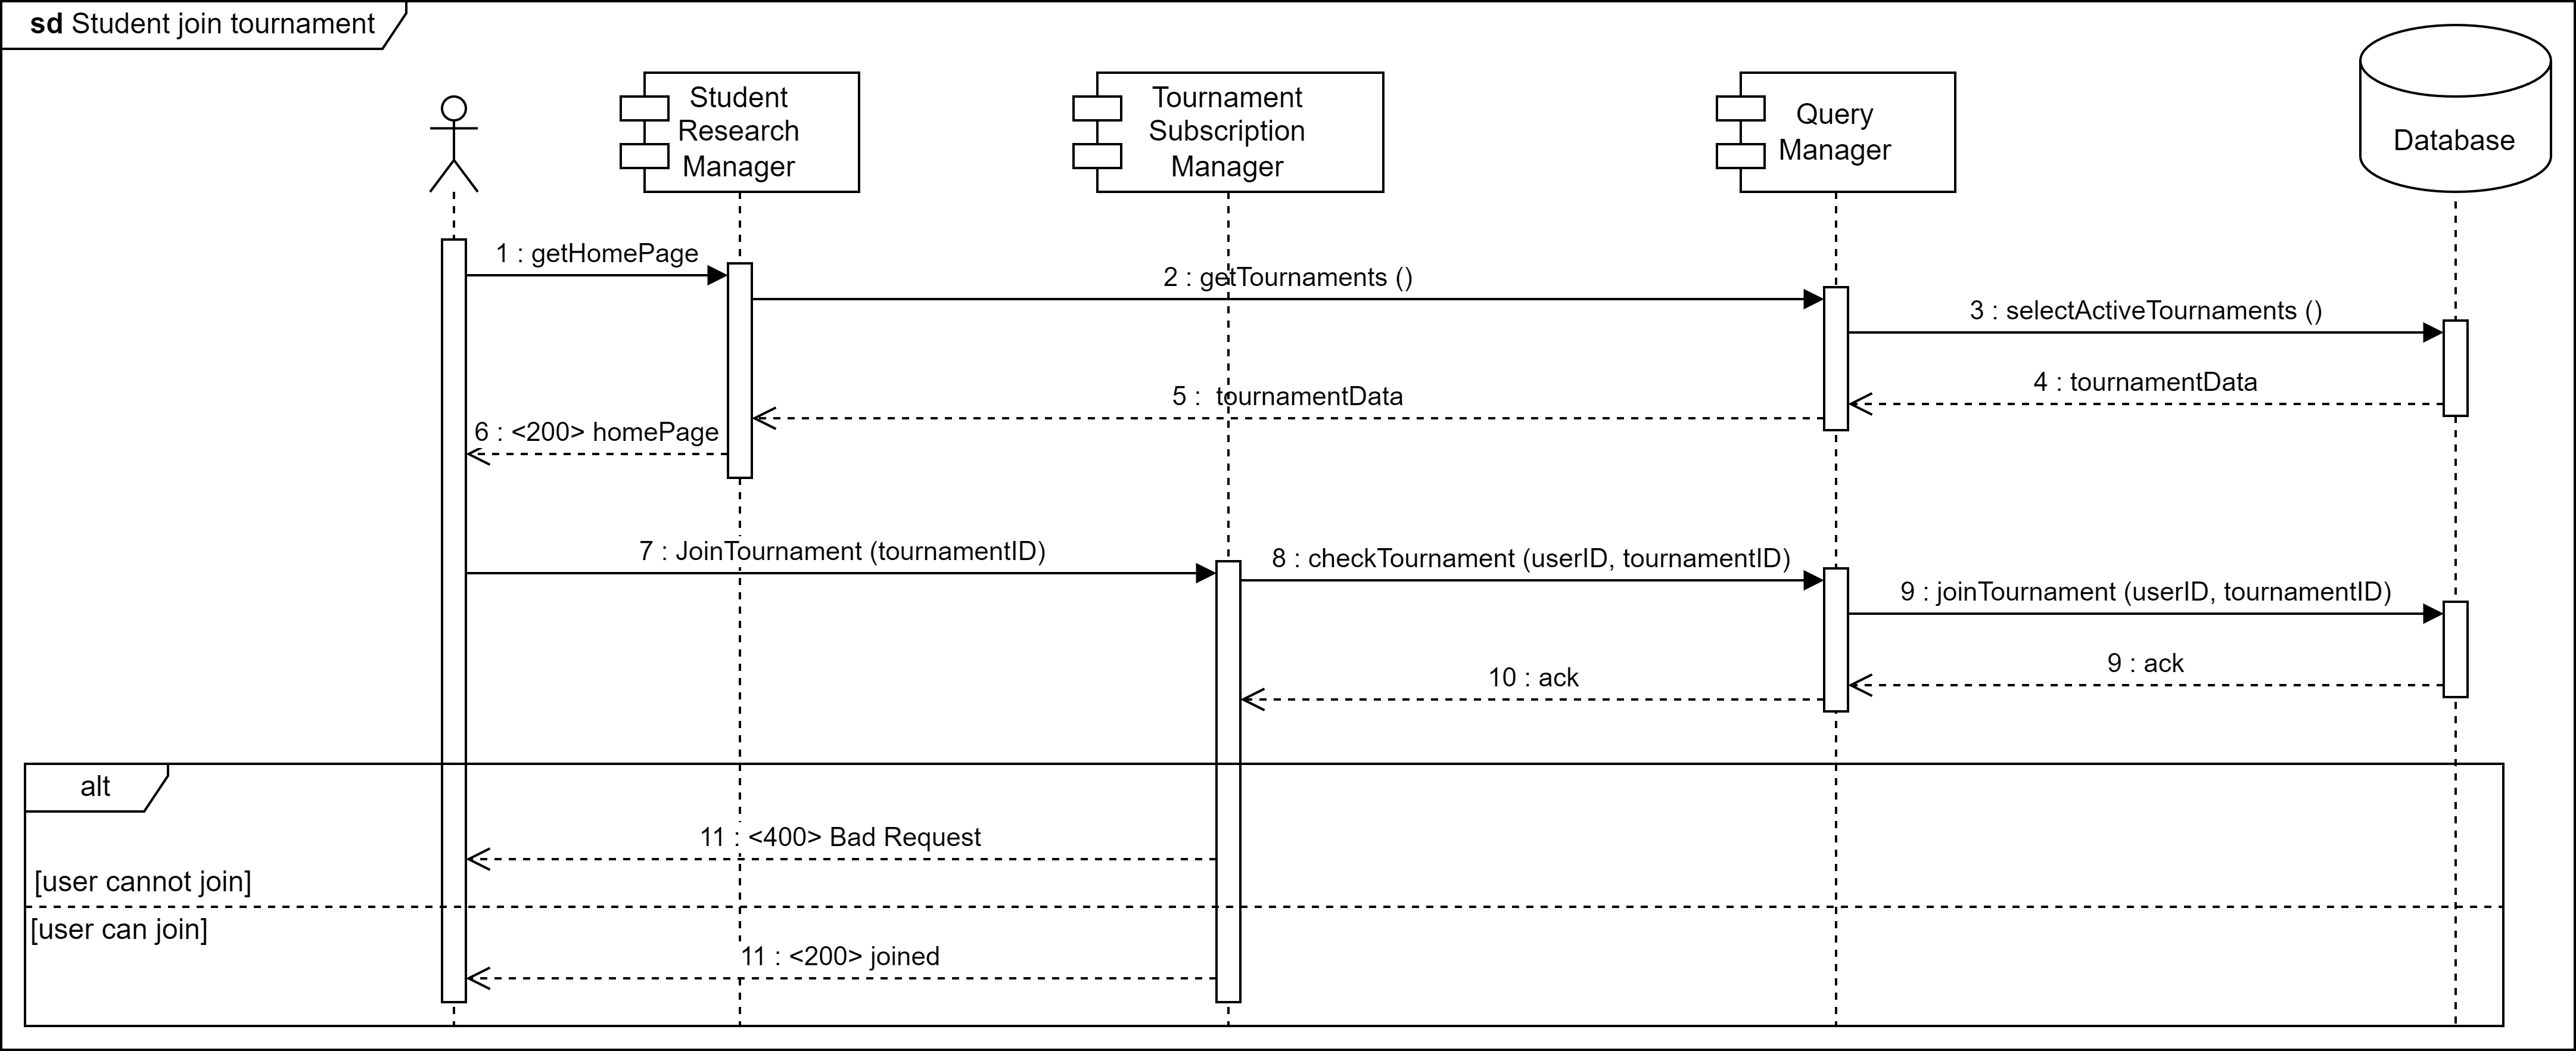
\includegraphics[width=1.0\linewidth]{images/sjtrv.png}
    \end{figure}

    \paragraph*{Student search tournament}
    In this case the actor is a registered student that wants to search for a specific tournament based on a keyword. 
    After accessing the search page the student can finally search the desired tournament. 
    The system returns all the tournaments linked with the searched keyword or a null list if no tournament match the requirements. 
    \begin{figure}[H]
        \centering
        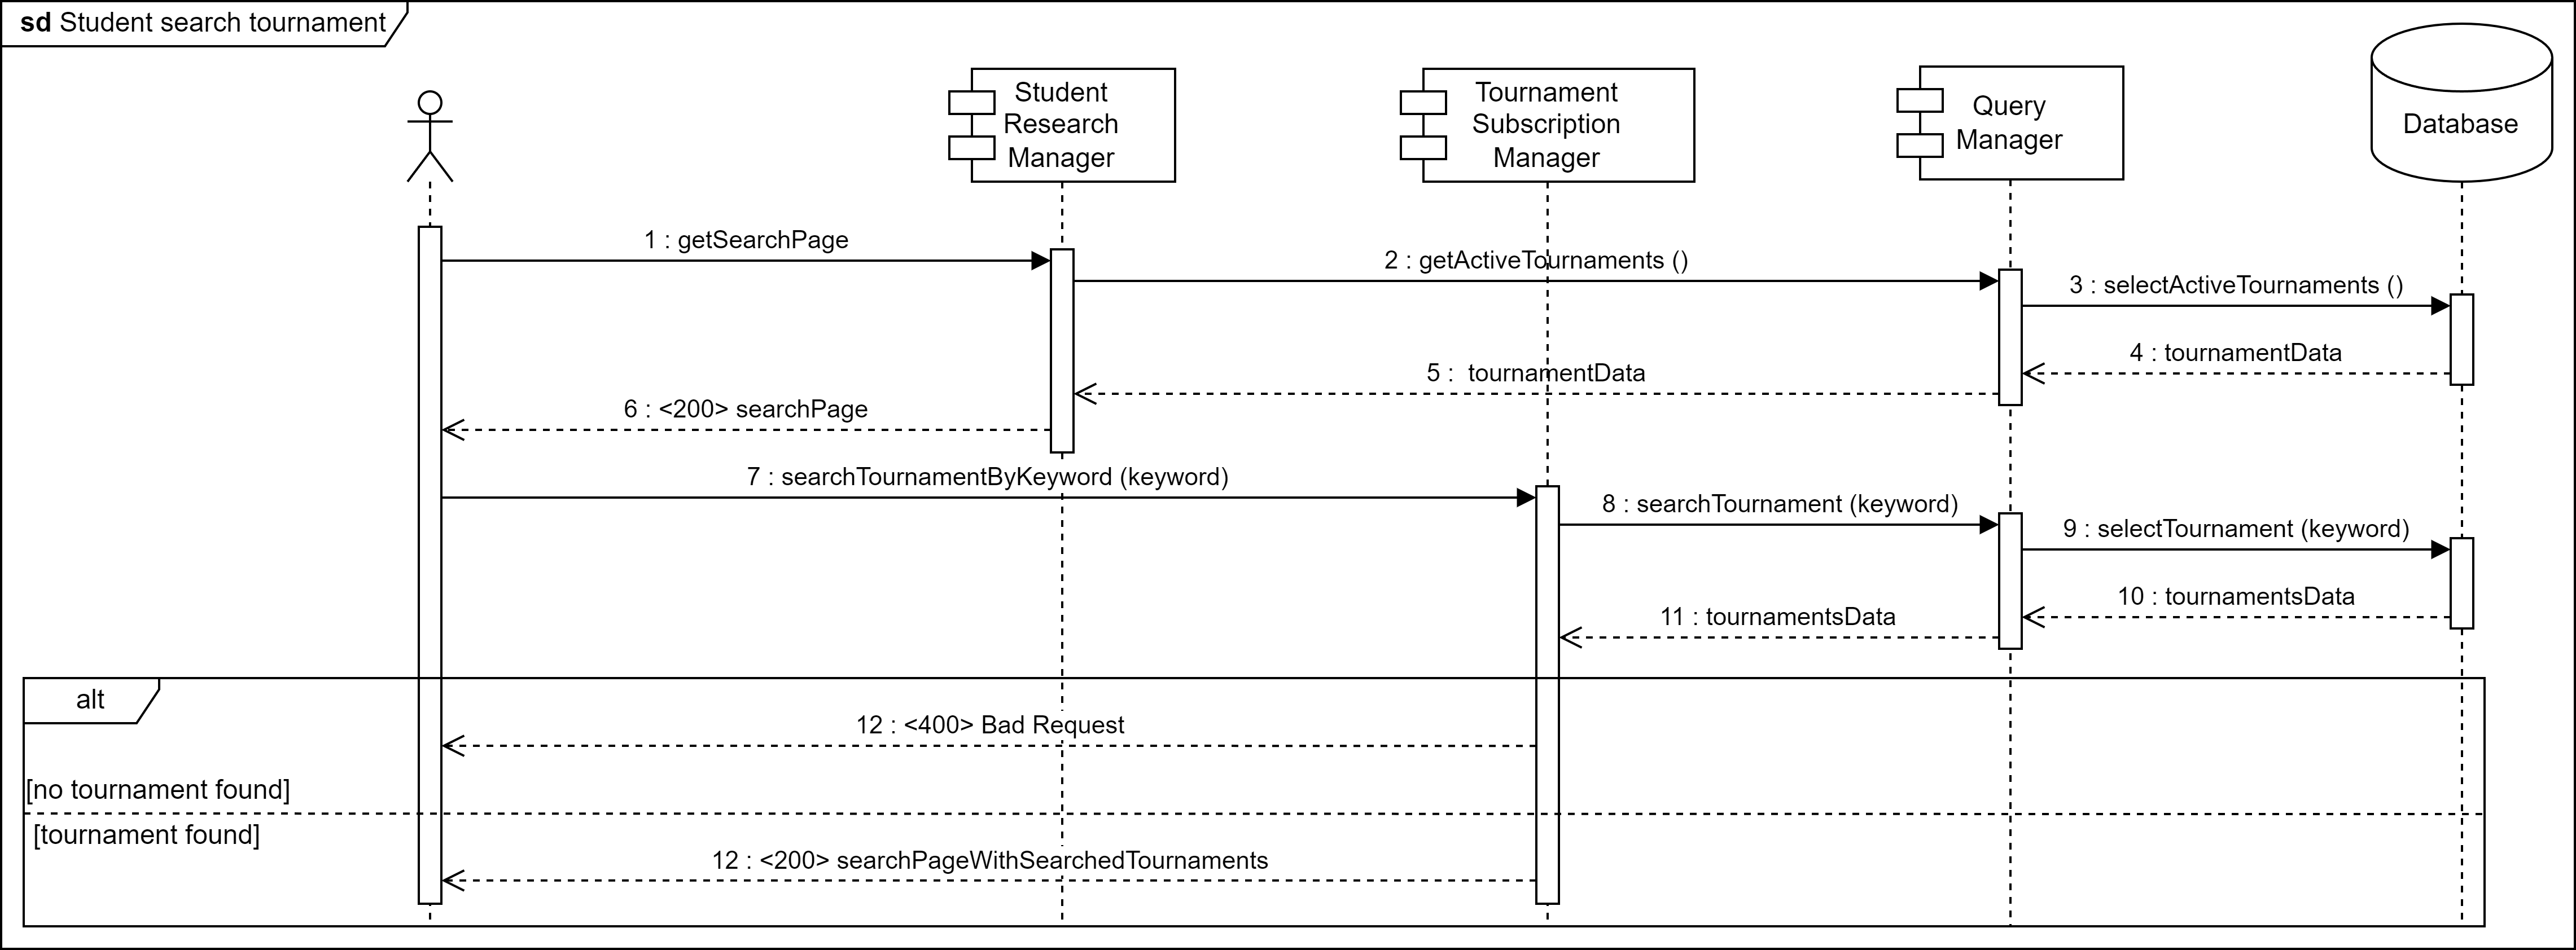
\includegraphics[width=1.0\linewidth]{images/sstrv.png}
    \end{figure}

    \paragraph*{Student join battle}
    In this case the actor is a registered student that wants to join a battle within a tournament in which he is enrolled. 
    After accessing the tournament details page the user clicks on the button to join the battle alone or in a team. 
    If the user is allowed to do the desired enrollment he can finally join the battle. 
    \begin{figure}[H]
        \centering
        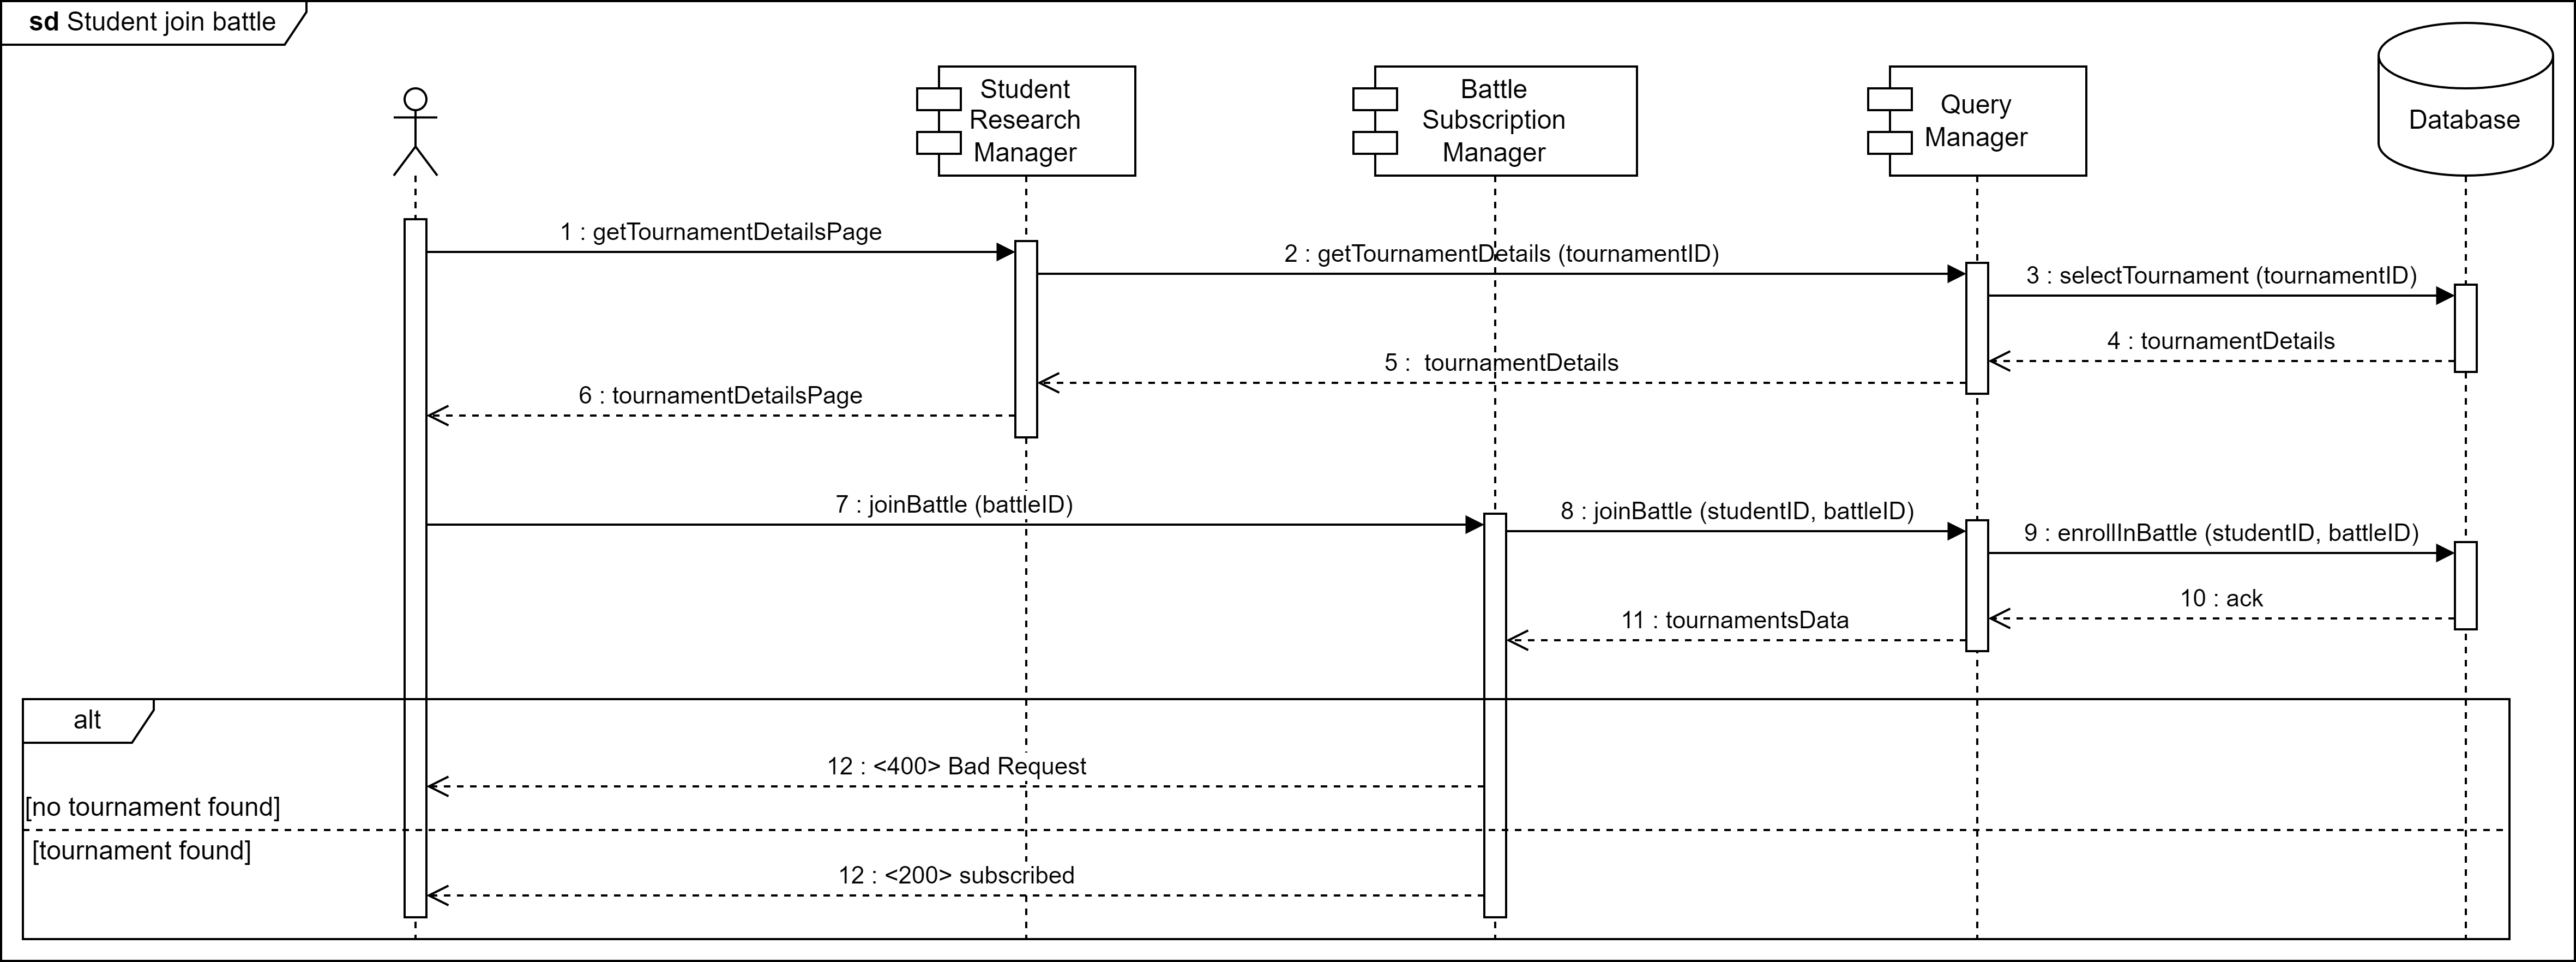
\includegraphics[width=1.0\linewidth]{images/sjbrv.png}
    \end{figure}

    \paragraph*{User checks tournament leaderboard}
    In this case the user is a registered student that wants to check the leaderboard of a tournament. 
    After accessing the enrolled page and consequently the tournament details page the student can access the leaderboard page of the selected tournament. 
    \begin{figure}[H]
        \centering
        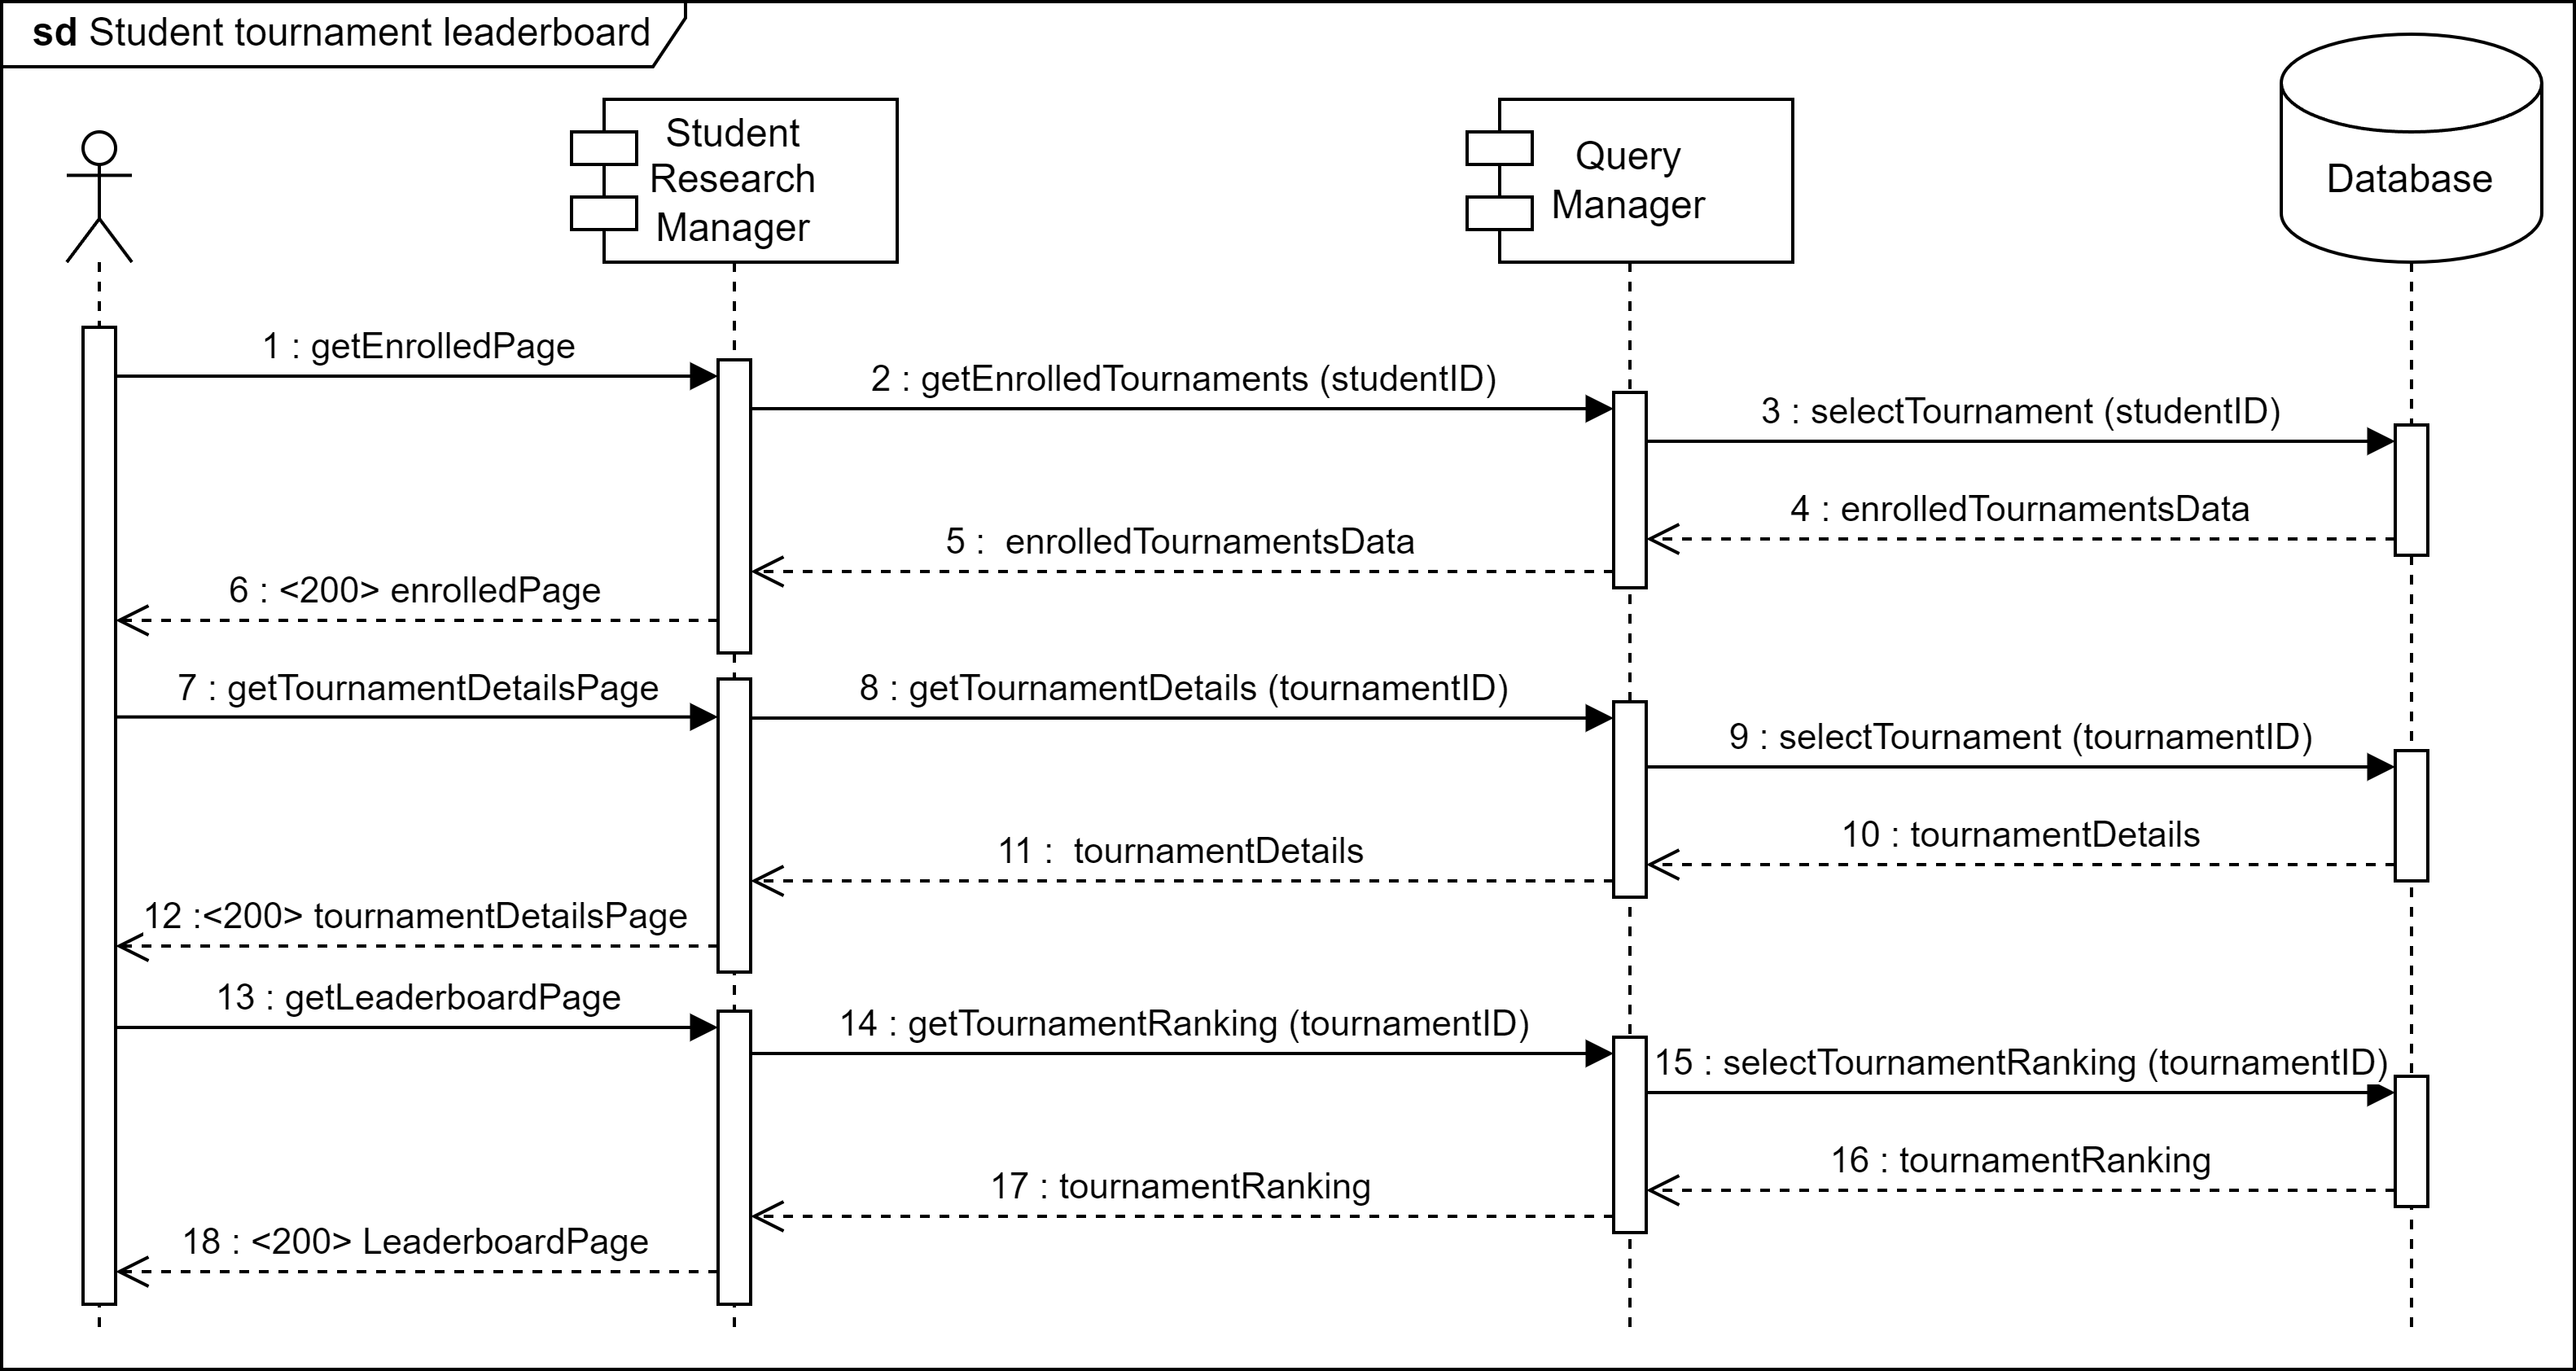
\includegraphics[width=1.0\linewidth]{images/stlrv.png}
    \end{figure}

    \paragraph*{User checks battle leaderboard}
    In this case the user is a registered student that wants to check the leaderboard of a tournament. 
    After accessing the enrolled page and consequently the tournament details page the student can access the leaderboard page of the selected tournament. 
    After this he can click on the button linked to the desired battle within the selected tournament. 
    \begin{figure}[H]
        \centering
        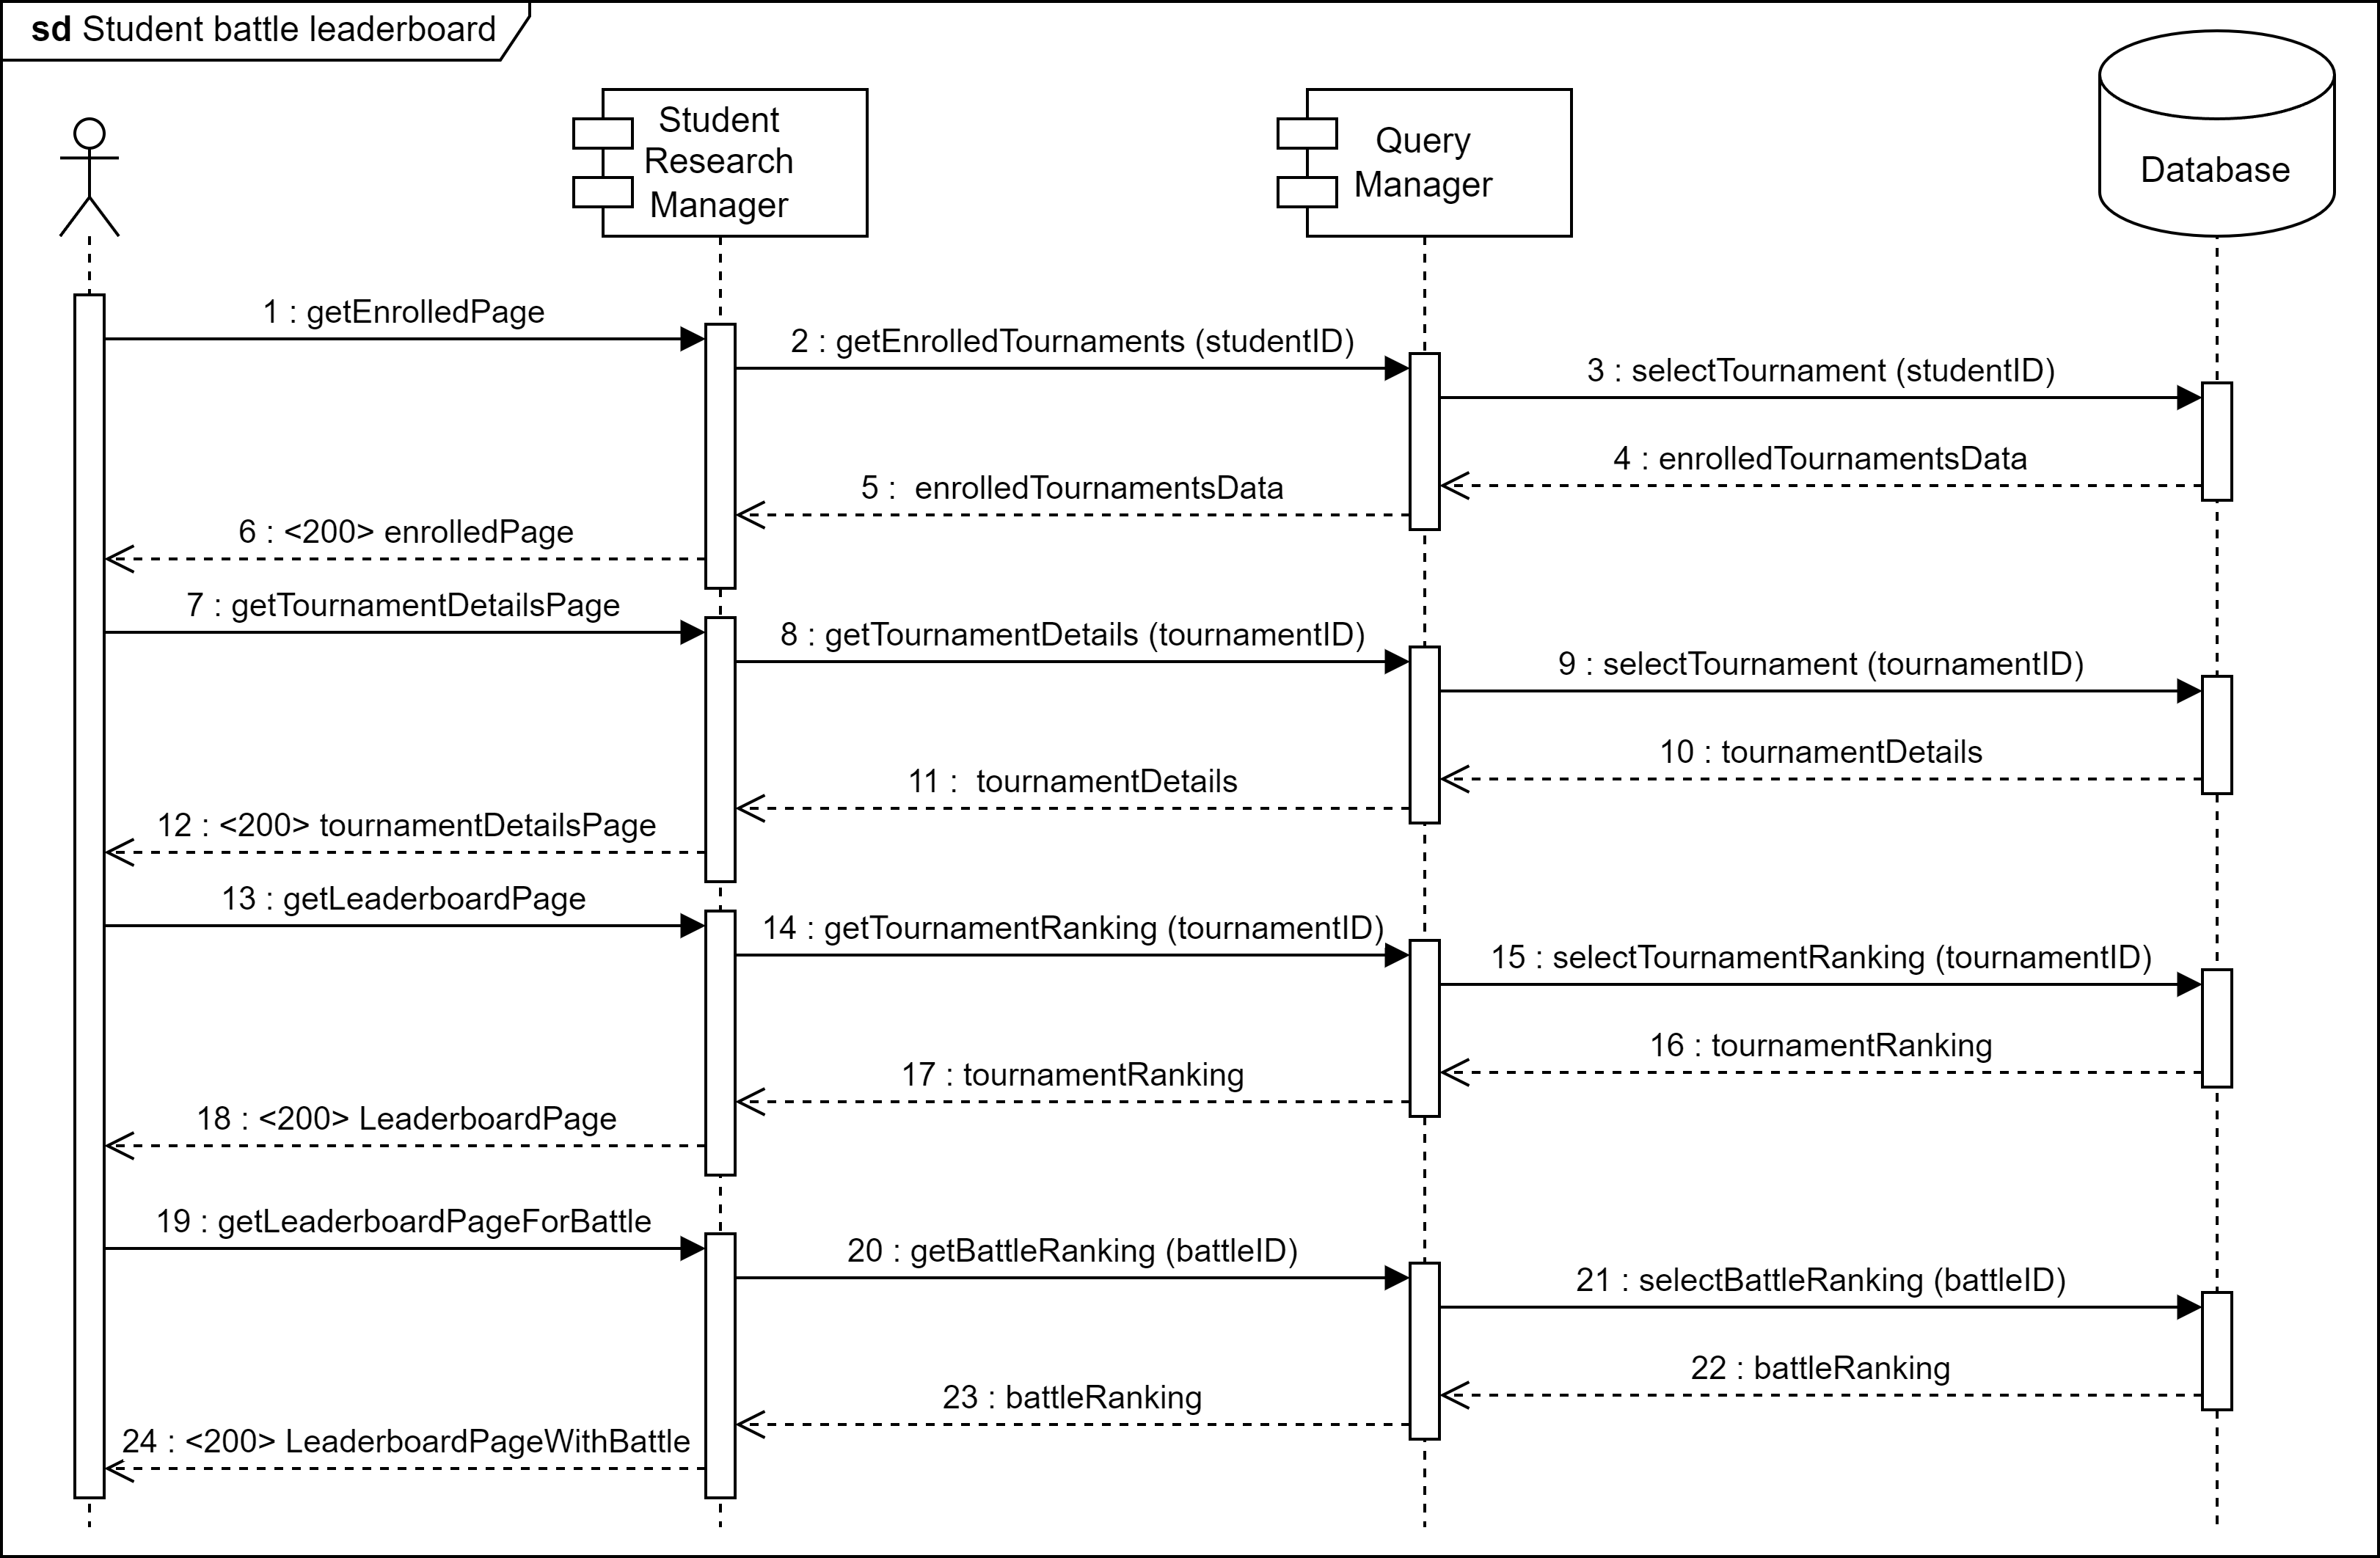
\includegraphics[width=1.0\linewidth]{images/sblrv.png}
    \end{figure}

    \subsection{Educator's runtime view}
    In this section we list all possible actions for the educator along with the runtime view associated with each one. 
    \paragraph*{Educator signup}
    In this case the actor is an unregistered educator that is trying to sign up in the system.
    After accessing the corresponding page the educator submits all the required information to the educator account manager component that cheks the data. 
    If the user is not already register it creates a new educator after the email verification. 
    \begin{figure}[H]
        \centering
        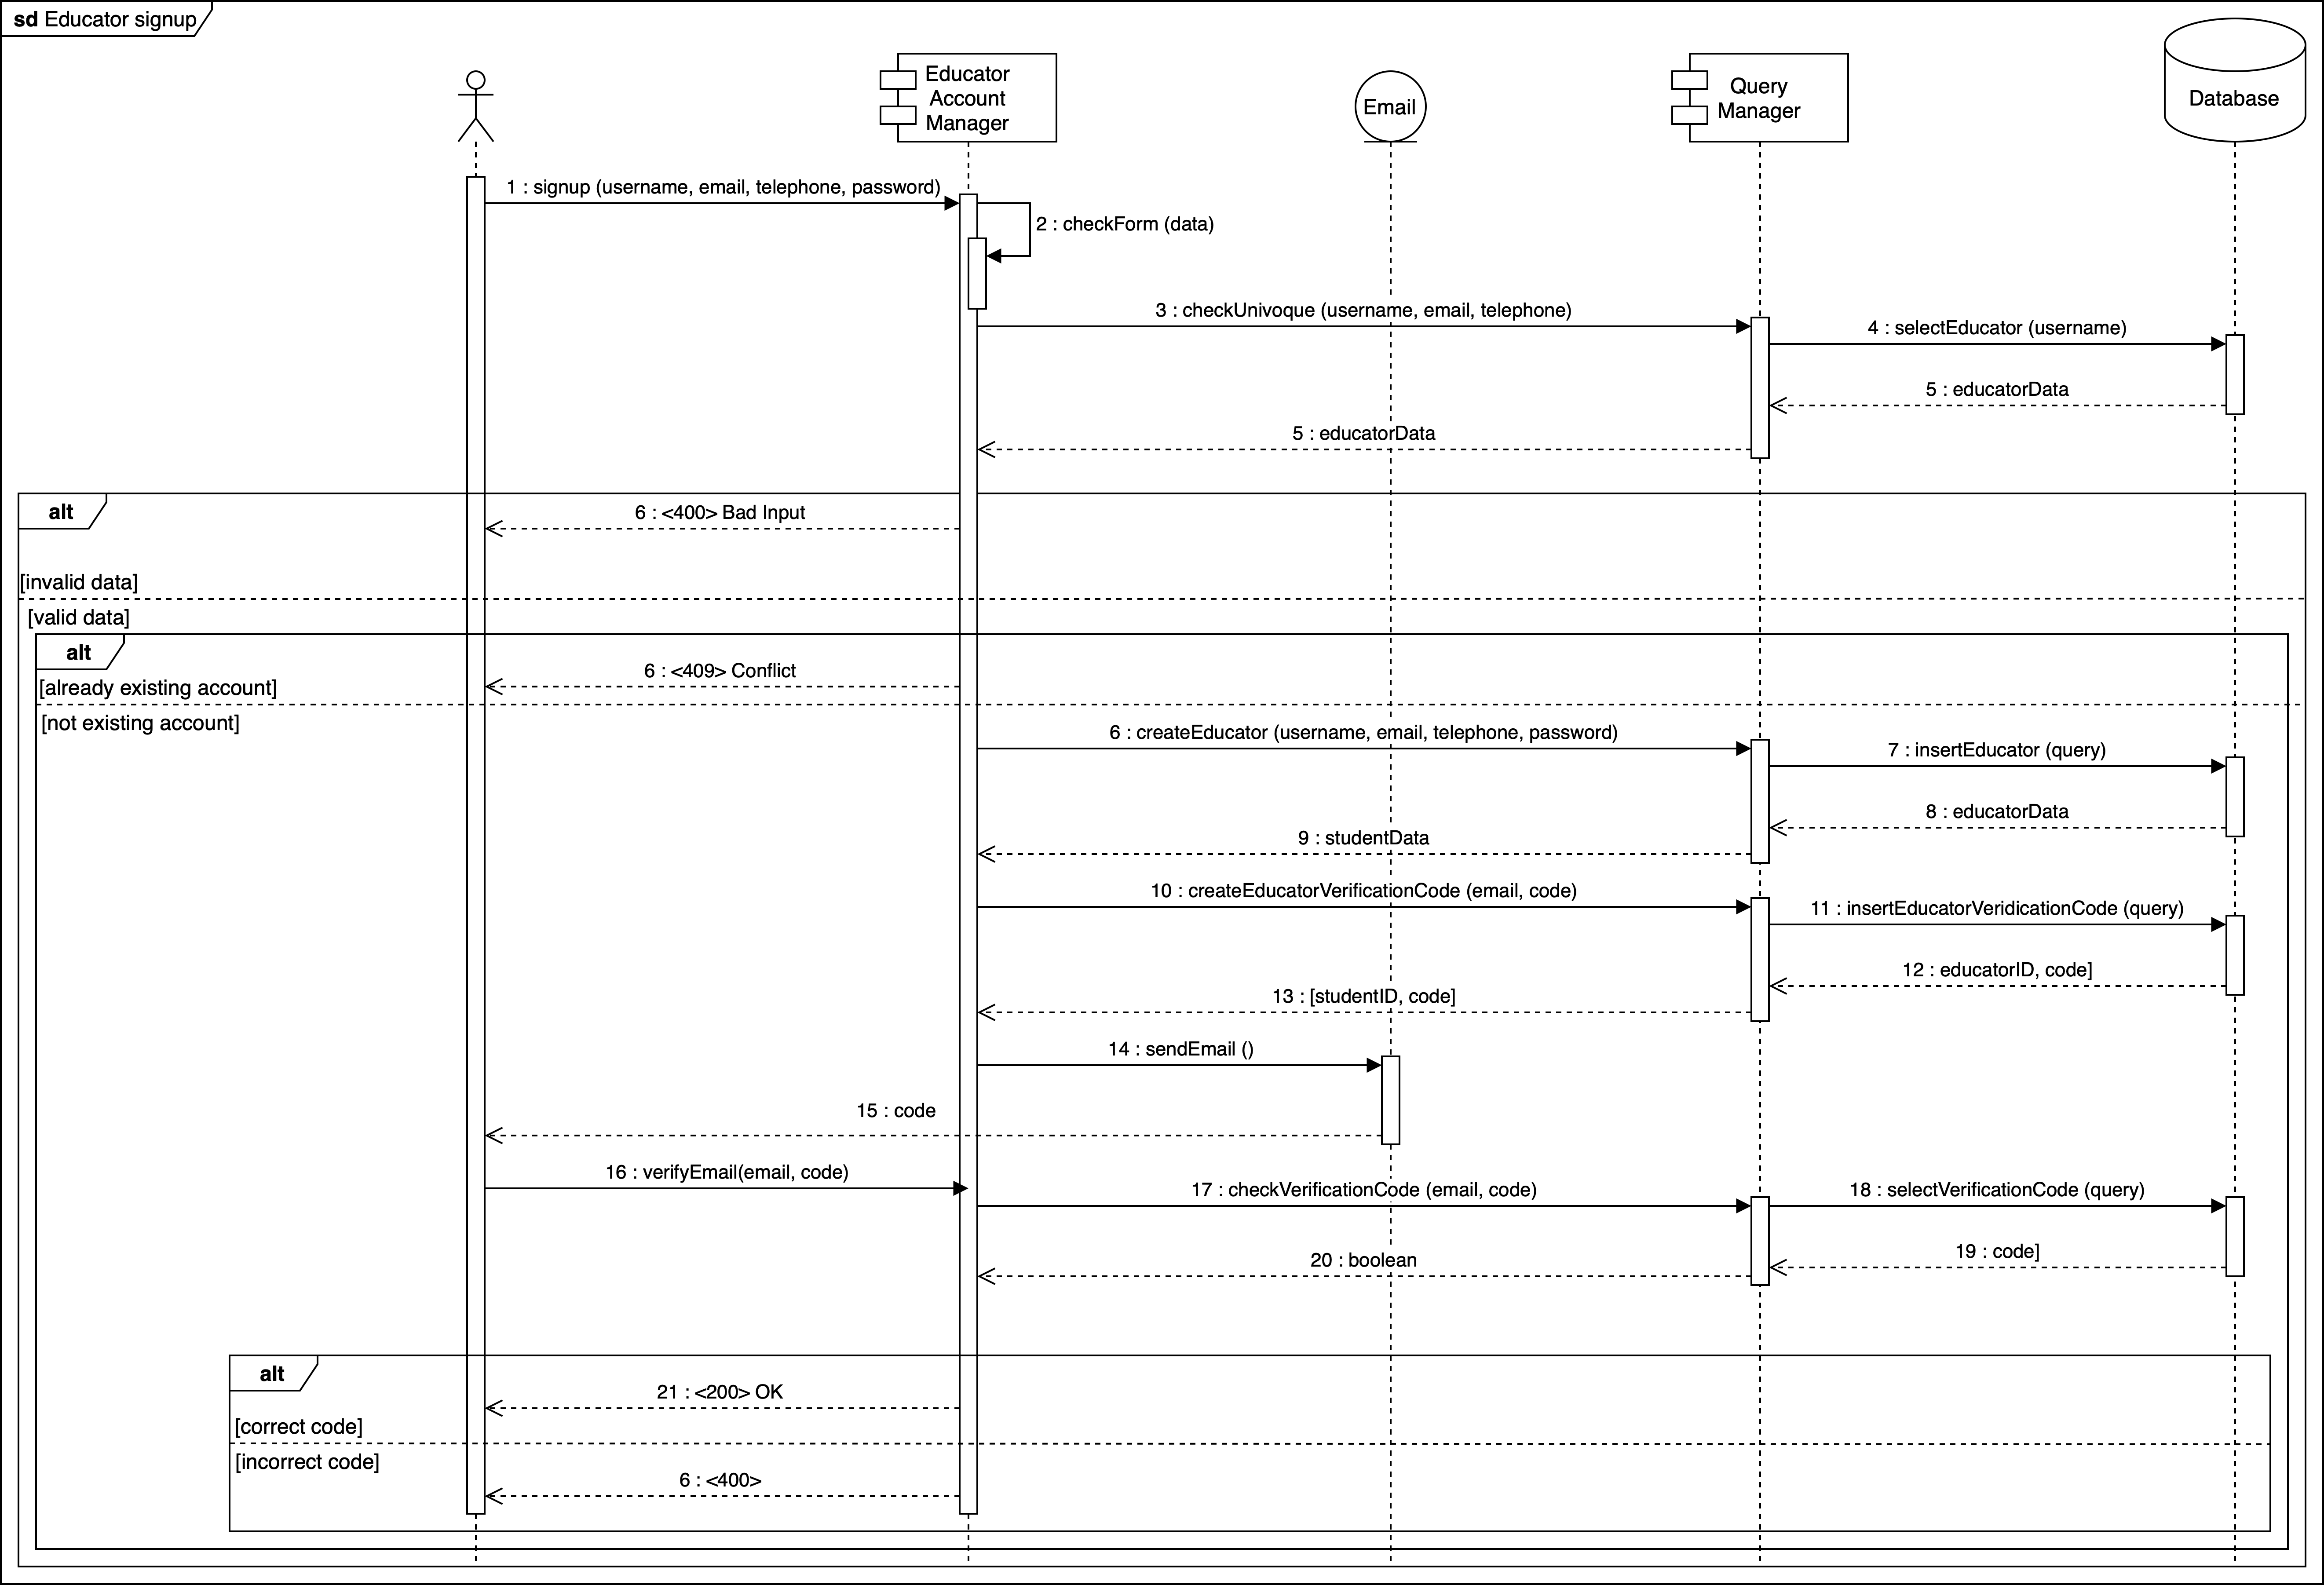
\includegraphics[width=1.0\linewidth]{images/esrv.png}
    \end{figure}

    \paragraph*{Educator log in}
    \begin{figure}[H]
        \centering
        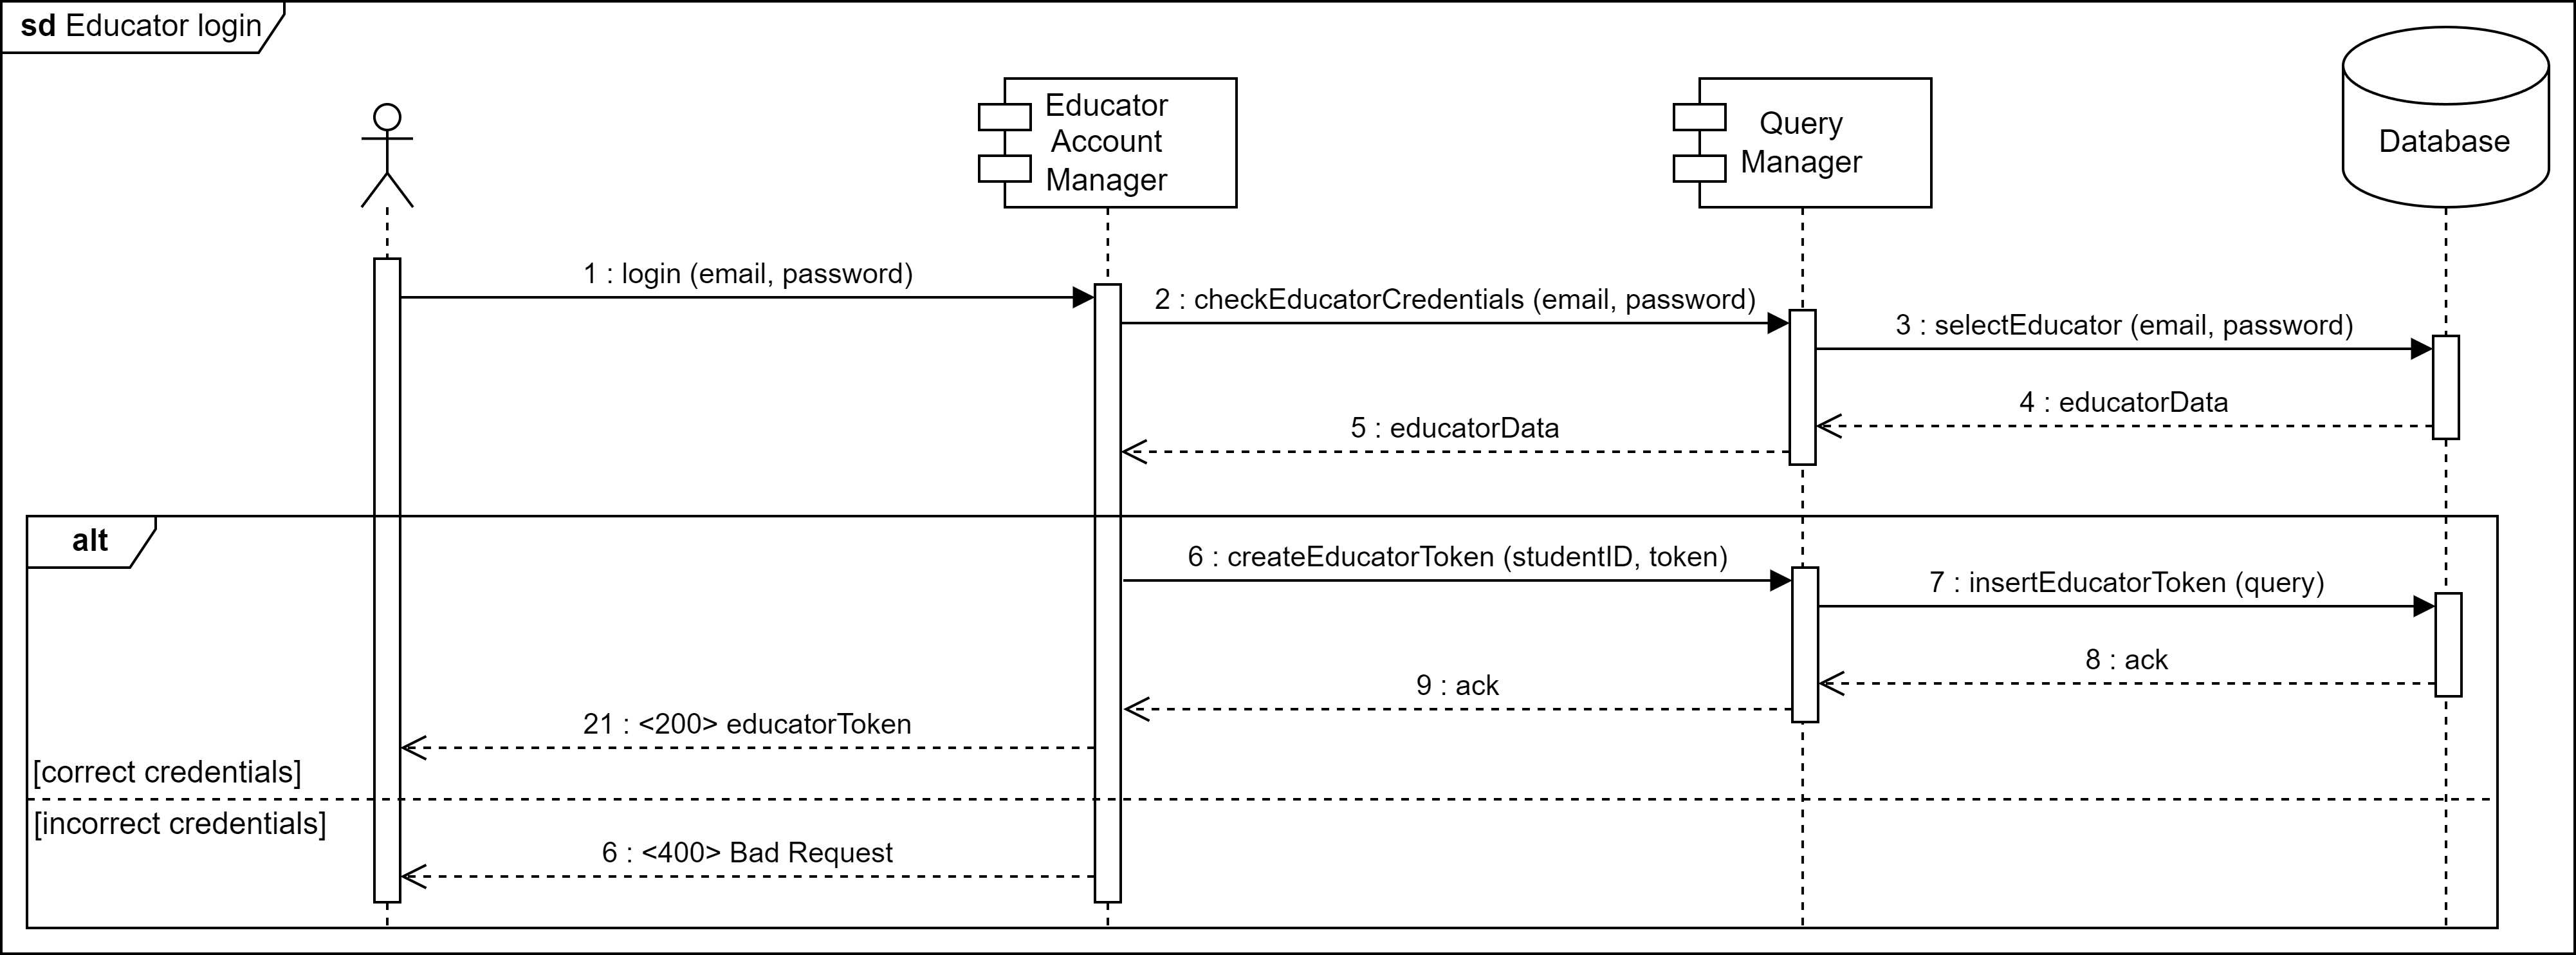
\includegraphics[width=1.0\linewidth]{images/elirv.png}
    \end{figure}
    In this case the actor is a registered educator that wants to log in into the system. 
    After accessing the corresponding page the educator submits all the required information to the educator account manager component that cheks the data. 
    If the inserted data are correct the educator can access all his possible actions. 

    \paragraph*{Educator profile}
    In this case the actor is a registered educator that wants to check his own profile. 
    The educator profile manager retrieves all the data linked to the educator and returns the complete page to the educator. 
    \begin{figure}[H]
        \centering
        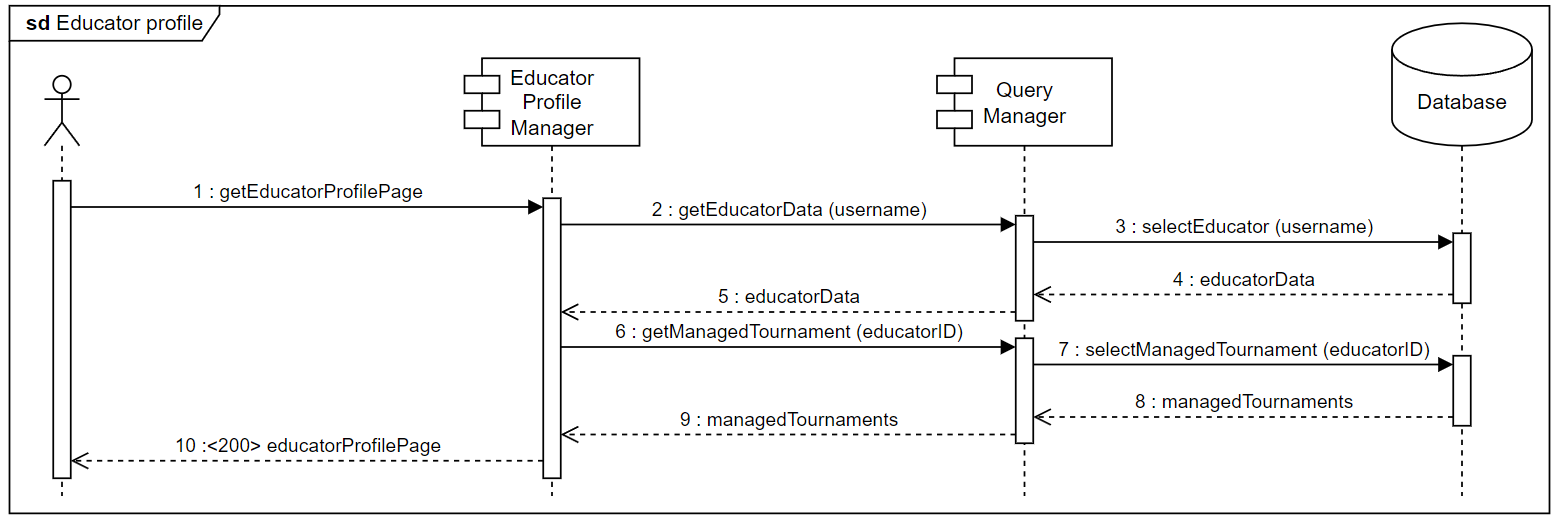
\includegraphics[width=1.0\linewidth]{images/eprv.png}
    \end{figure}

    \paragraph*{Educator home page}
    In this case the actor is a registered educator that wants to access the home page. 
    The educator research manager retrieves all the active tournaments from the database and return the home page with some tournaments. 
    \begin{figure}[H]
        \centering
        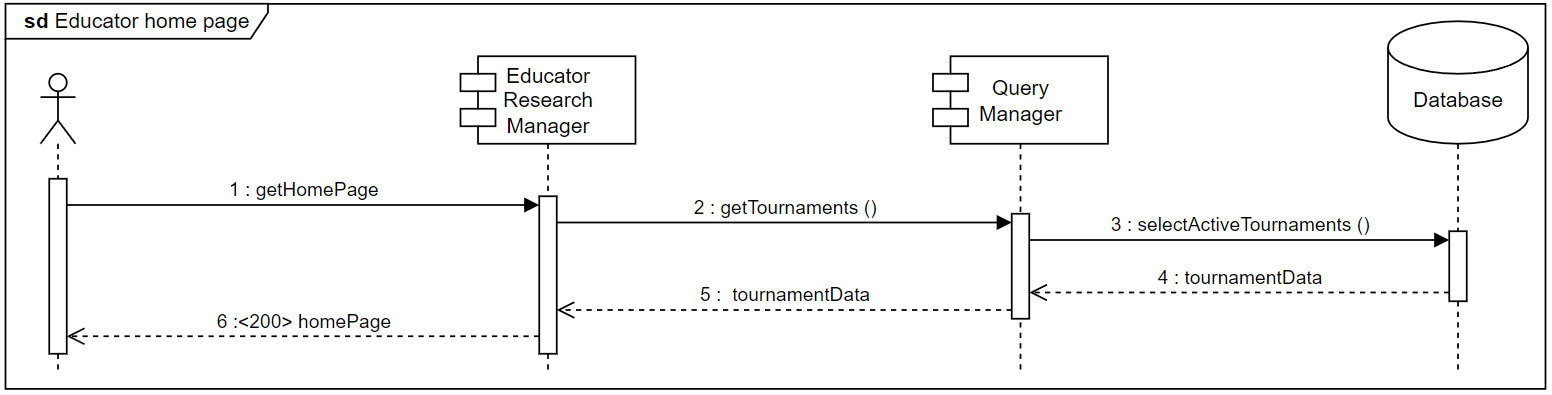
\includegraphics[width=1.0\linewidth]{images/ehprv.png}
    \end{figure}

    \paragraph*{Educator search tournament}
    In this case the actor is a registered educator that wants to search for a specific tournament based on a keyword. 
    After accessing the search page the educator can finally search the desired tournament. 
    The system returns all the tournaments linked with the searched keyword or a null list if no tournament match the requirements. 
    \begin{figure}[H]
        \centering
        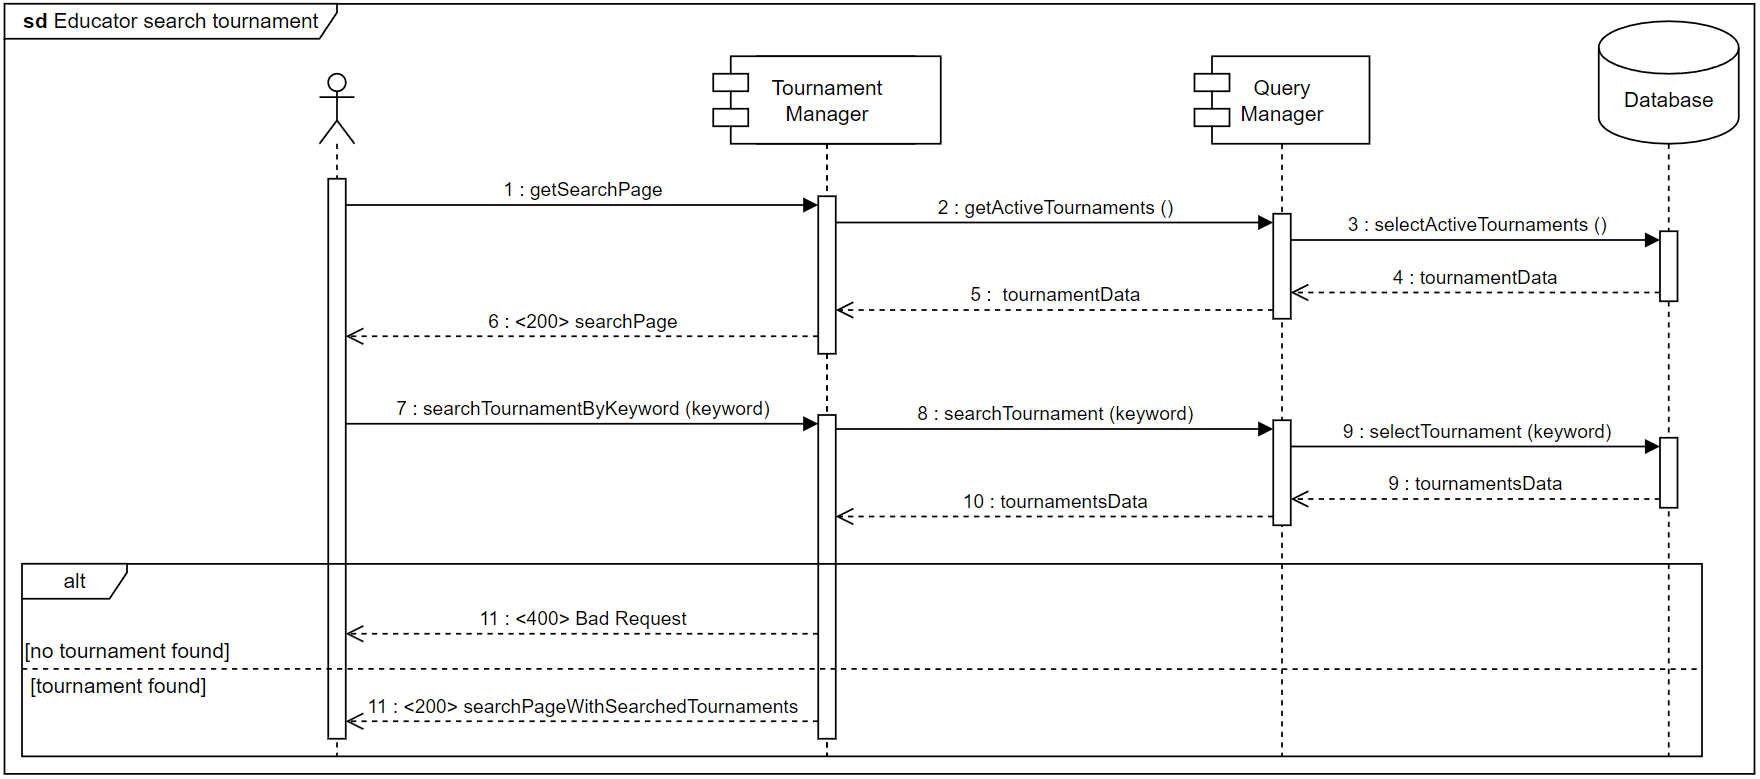
\includegraphics[width=1.0\linewidth]{images/estrv.png}
    \end{figure}

    \paragraph*{Educator create tournament}
    In this case the actor is an educator that wants to create a new tournament. 
    After accessing the create tournament page and compiling all the requested information he sumbits the data. 
    The system check all information and returns the state of the requested action (the creation of the tournament). 
    \begin{figure}[H]
        \centering
        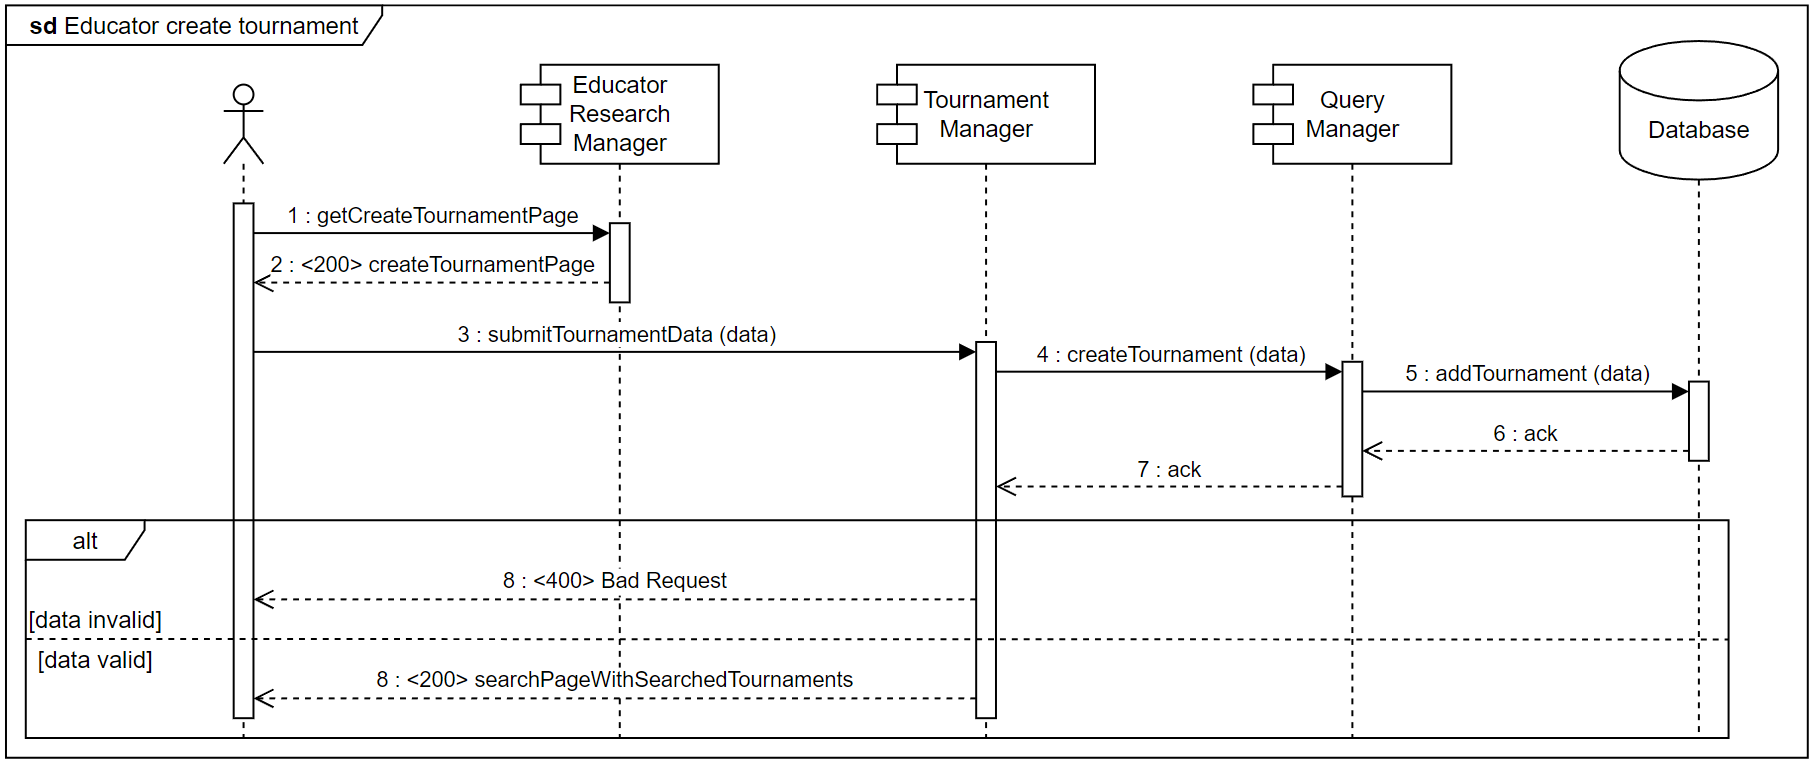
\includegraphics[width=1.0\linewidth]{images/ectrv.png}
    \end{figure}

    \paragraph*{Educator manage tournament}
    In this case the actor is an educator that wants to manage an already existing tournament. 
    After accessing the manage tournament page he clicks on the desired tournament. 
    The system check if the user is allowed to check the tournament and returns the same page with all the details. 
    \begin{figure}[H]
        \centering
        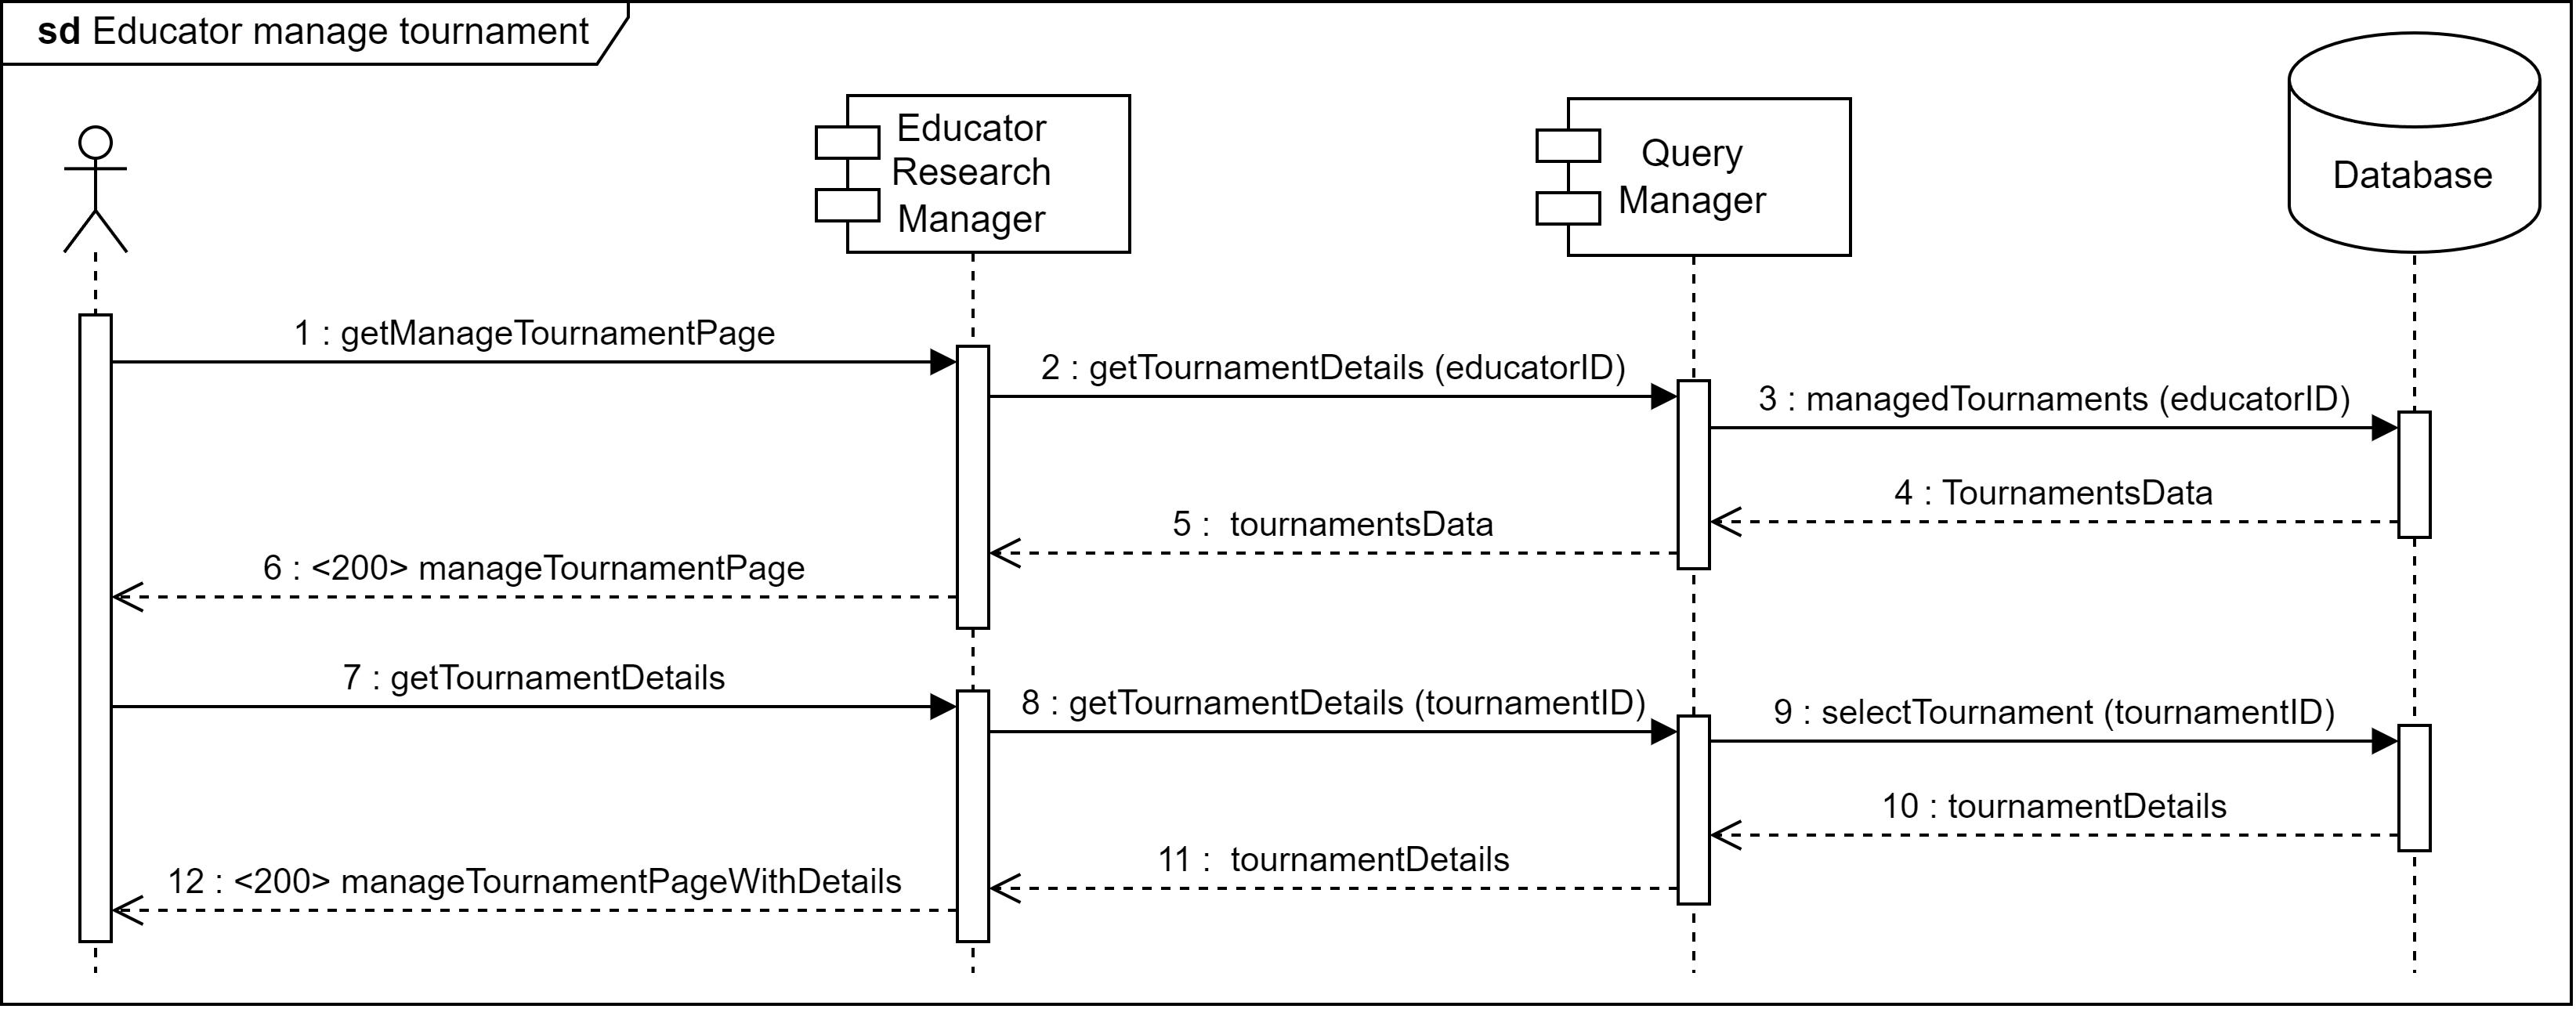
\includegraphics[width=1.0\linewidth]{images/emtrv.png}
    \end{figure}

    \paragraph*{Educator add battle}
    In this case the actor is an educator that wants to manage an already existing tournament by adding a battle. 
    After accessing the manage tournament page he clicks on the desired tournament. 
    The system check if the user is allowed to check the tournament and returns the same page with all the details. 
    Now the educator can finally click on the add button to create a new battle within the tournament. 
    The system return the create battle page, and the educator can finally insert all the information regarding the battle. 
    If all data arre correct the system adds the new battle and notifies the educator. 
    \begin{figure}[H]
        \centering
        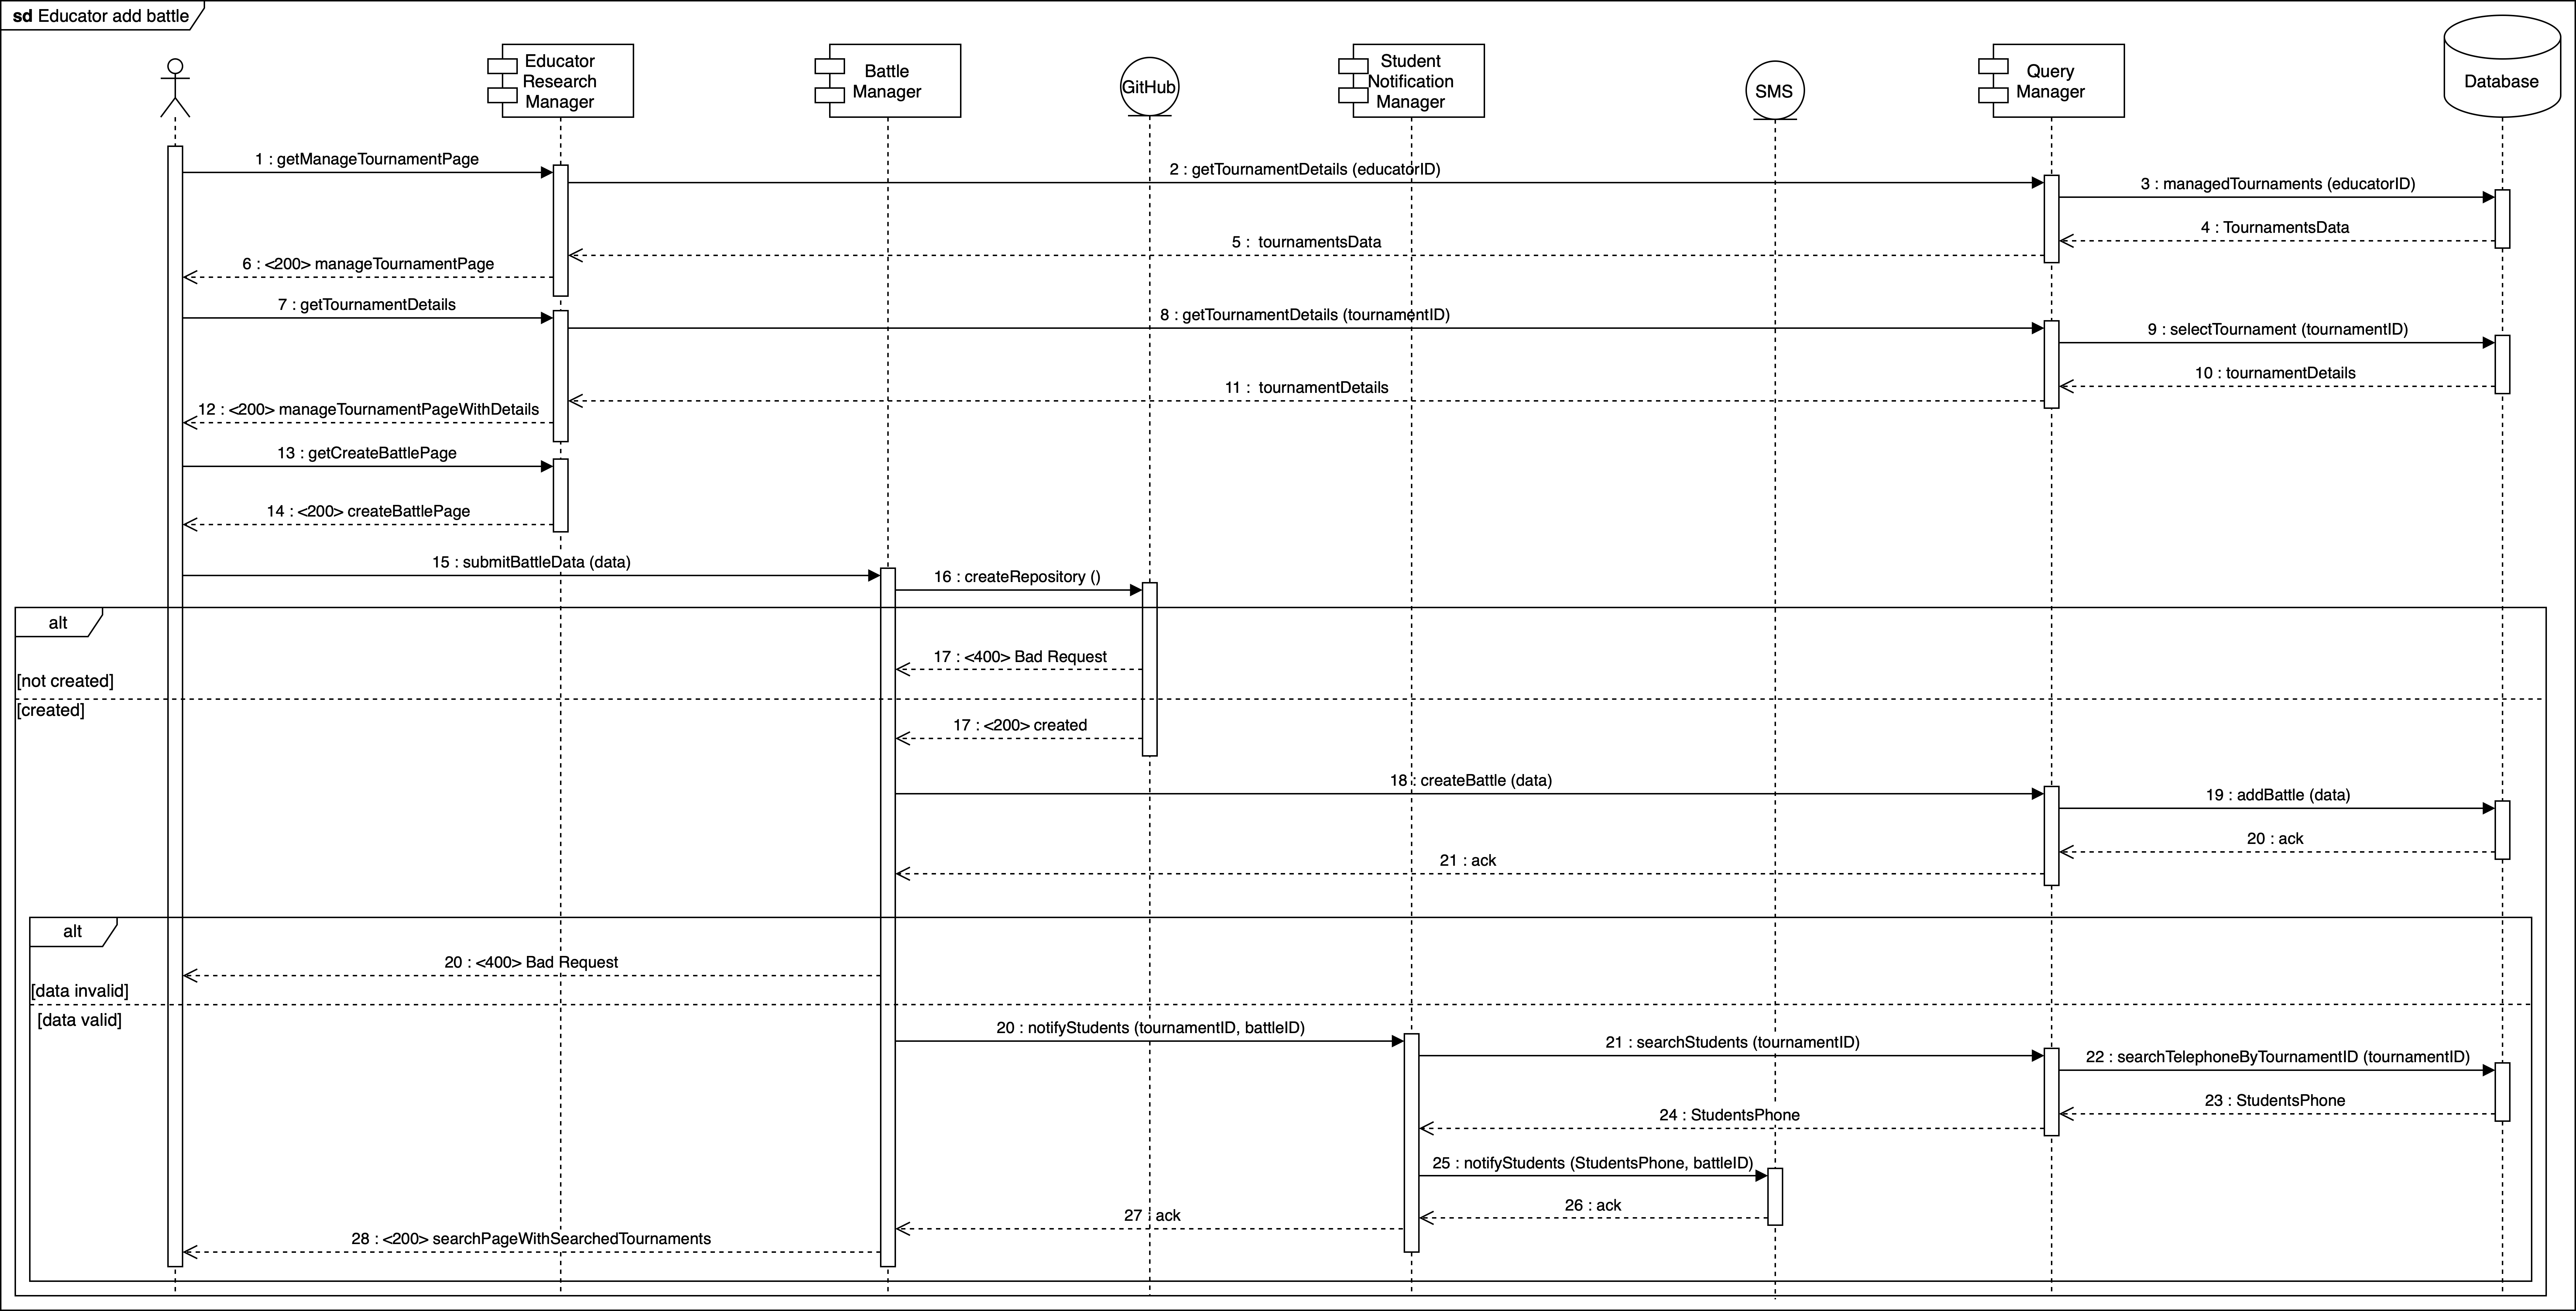
\includegraphics[width=1.0\linewidth]{images/eabrv.png}
    \end{figure}

    \paragraph*{Educator add collaborator}
    In this case the actor is an educator that wants to manage an already existing tournament by adding a collaborator. 
    After accessing the manage tournament page he clicks on the desired tournament. 
    The system check if the user is allowed to check the tournament and returns the same page with all the details. 
    Now the educator can finally click on the add collaborator button to invite other educators. 
    The educator sumbits the email and the system let him know if the collaborator is invited or not. 
    \begin{figure}[H]
        \centering
        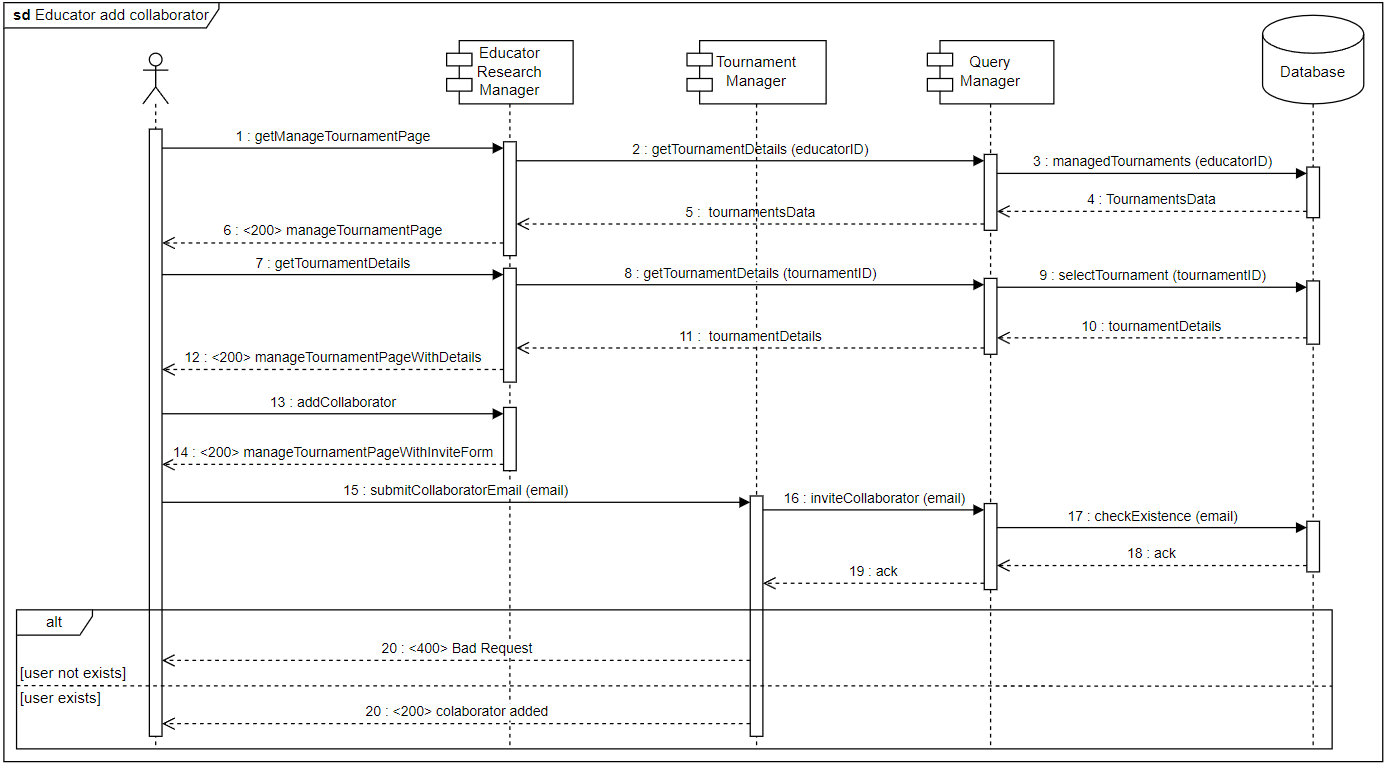
\includegraphics[width=1.0\linewidth]{images/eacrv.png}
    \end{figure}

    \paragraph*{Educator close tournament}
    In this case the actor is an educator that wants to manage an already existing tournament by closing it. 
    After accessing the manage tournament page he clicks on the desired tournament. 
    The system check if the user is allowed to check the tournament and returns the same page with all the details. 
    Now the educator can finally click on the close button. 
    The system nbotifies the educator on the status of the action. 
    \begin{figure}[H]
        \centering
        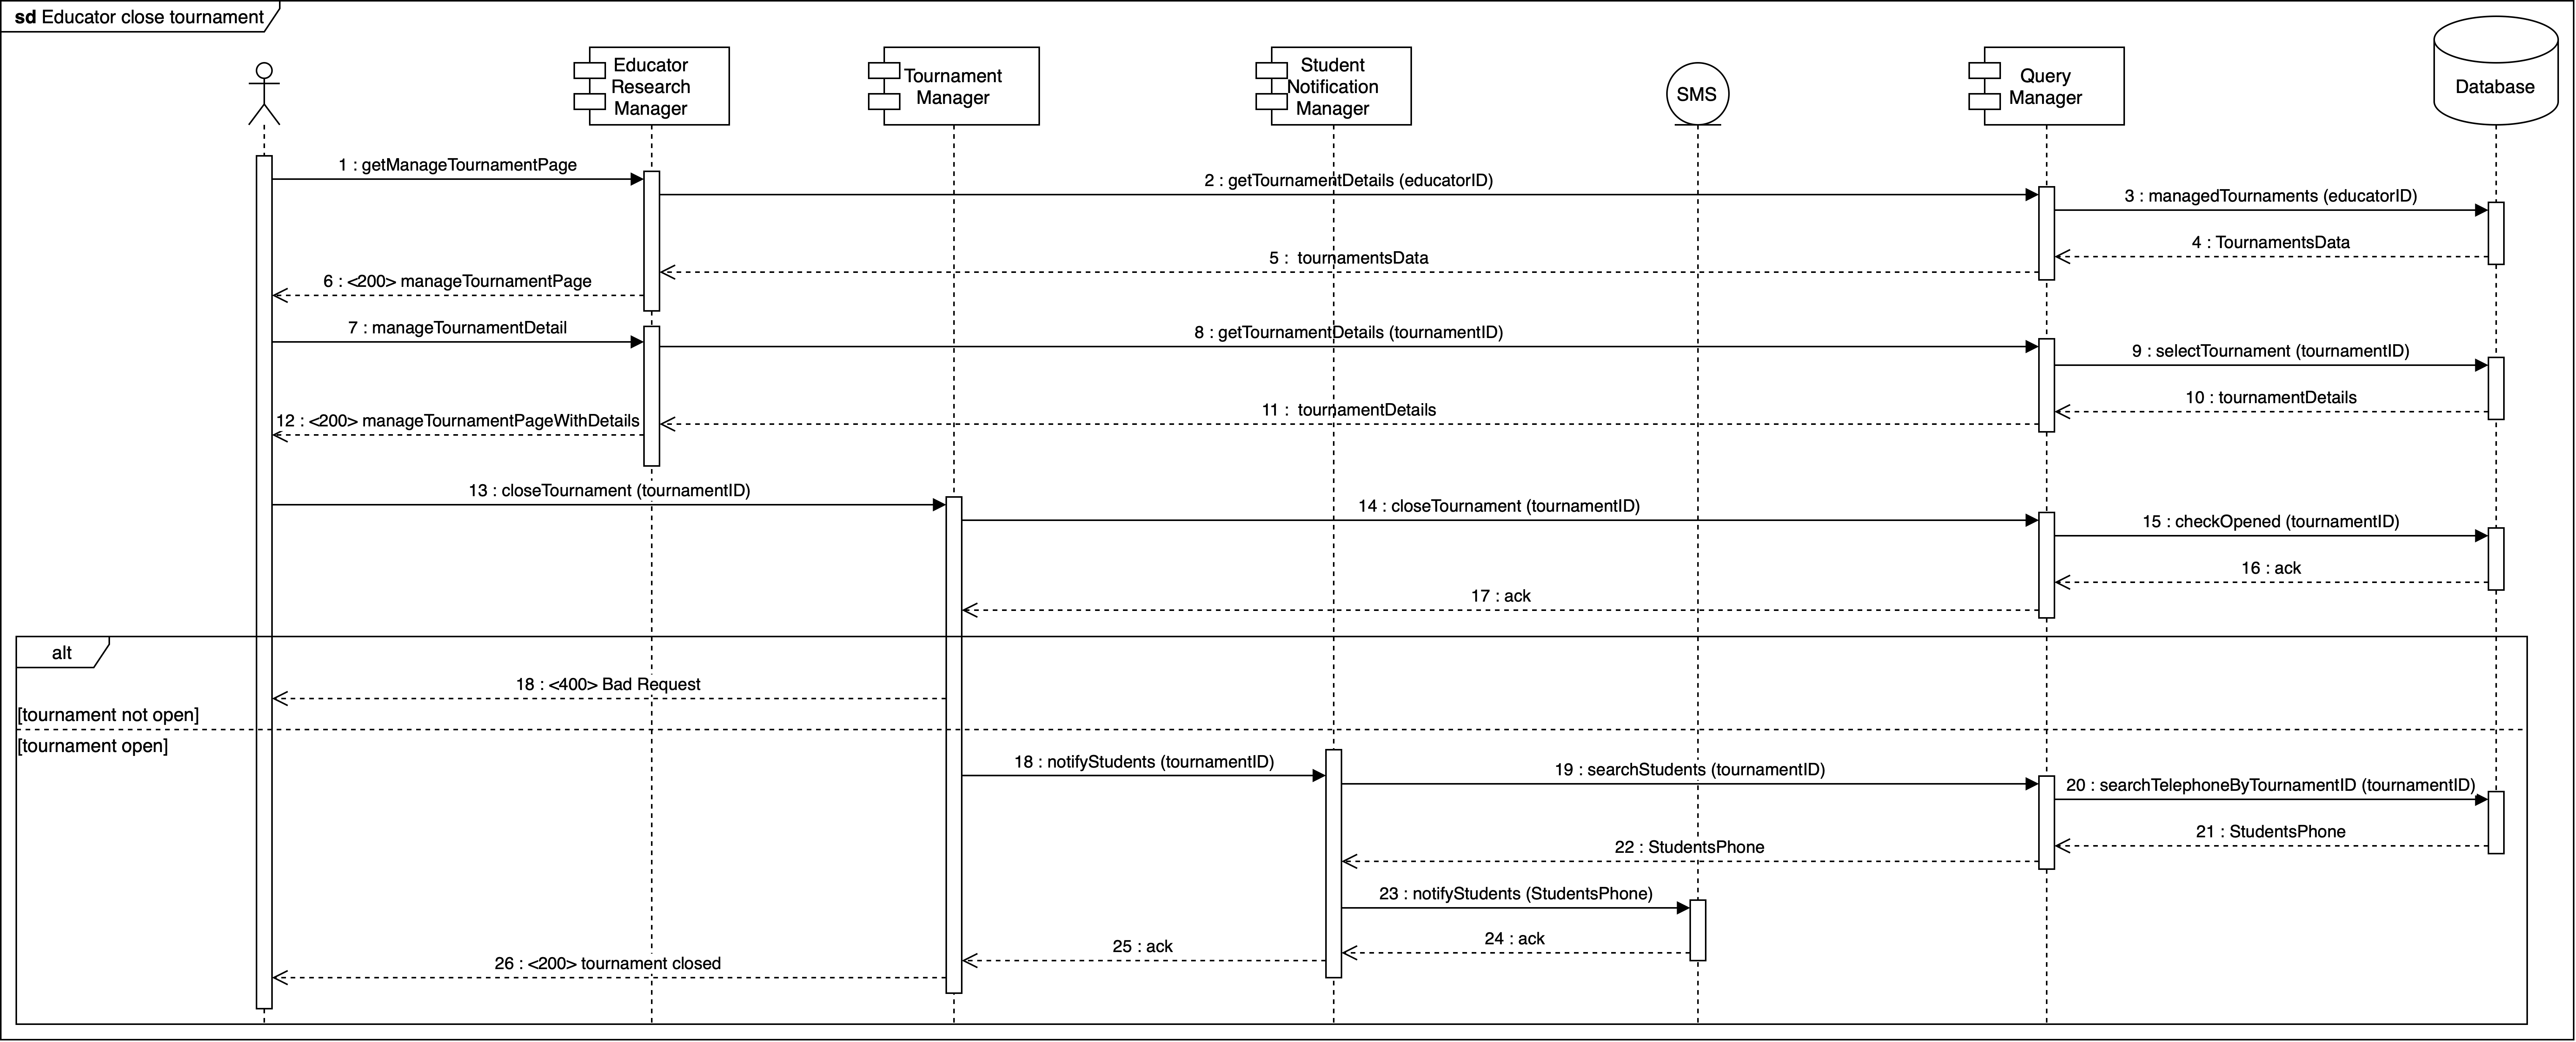
\includegraphics[width=1.0\linewidth]{images/ectrv1.png}
    \end{figure}

    \paragraph*{Educator personal evaluation}
    In this case the actor is an educato that wants to add the personal evaluation to a managed tournament. 
    After accessing the manage battle page and selecting the desired battle he can finally fill out the form with the evaluations.
    If all submitted values are correct the system insert these into the database and notifies the user with a message.
    \begin{figure}[H]
        \centering
        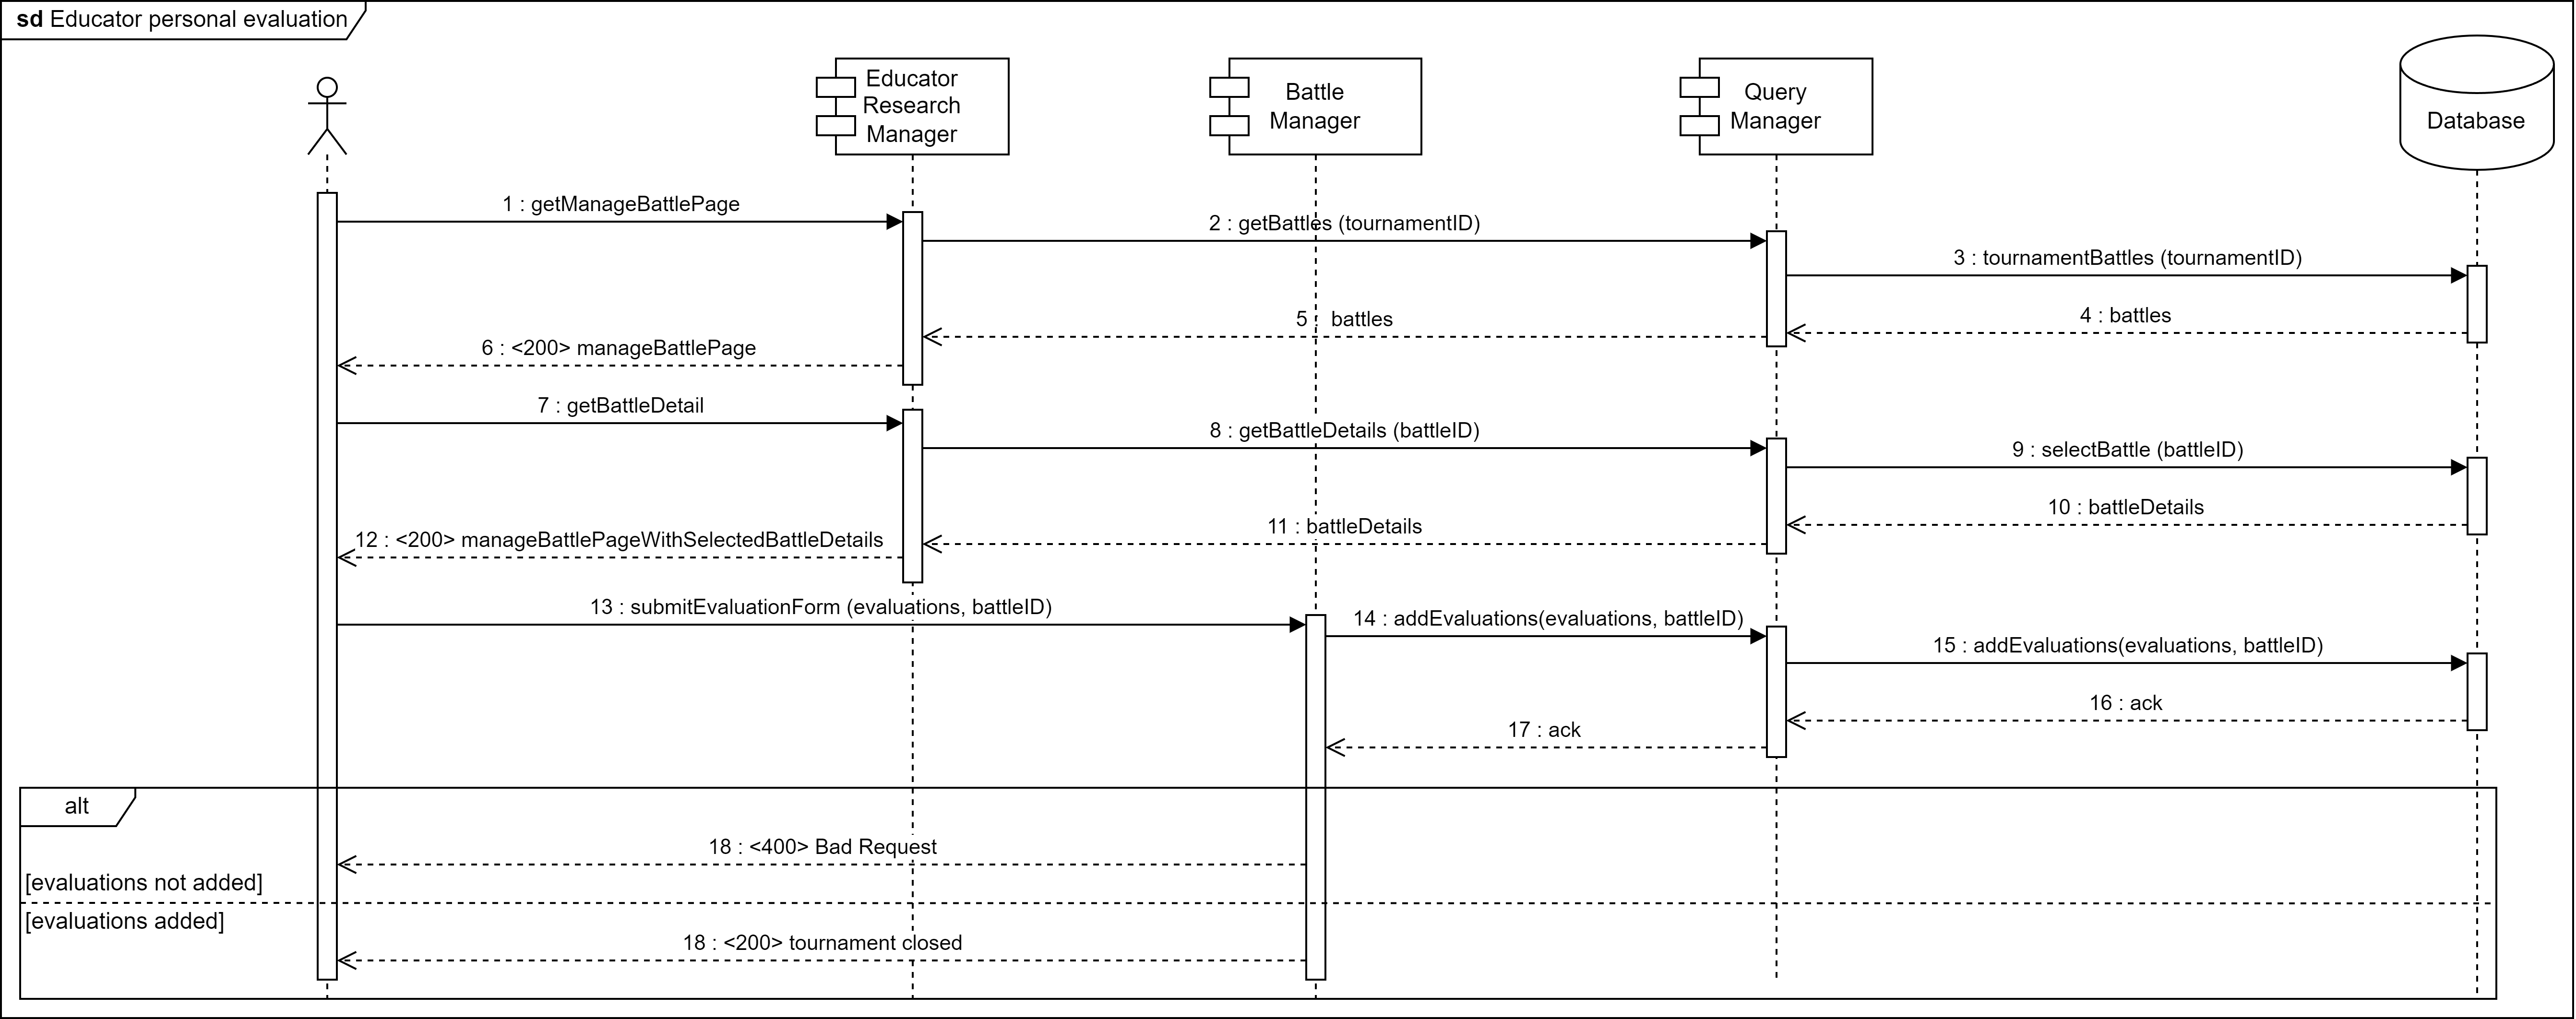
\includegraphics[width=1.0\linewidth]{images/eperv.png}
    \end{figure}

    \paragraph*{User checks tournament leaderboard}
    In this case the user is a registered student that wants to check the leaderboard of a tournament. 
    After accessing the search page and consequently the tournament details page the student can access the leaderboard page of the selected tournament. 
    \begin{figure}[H]
        \centering
        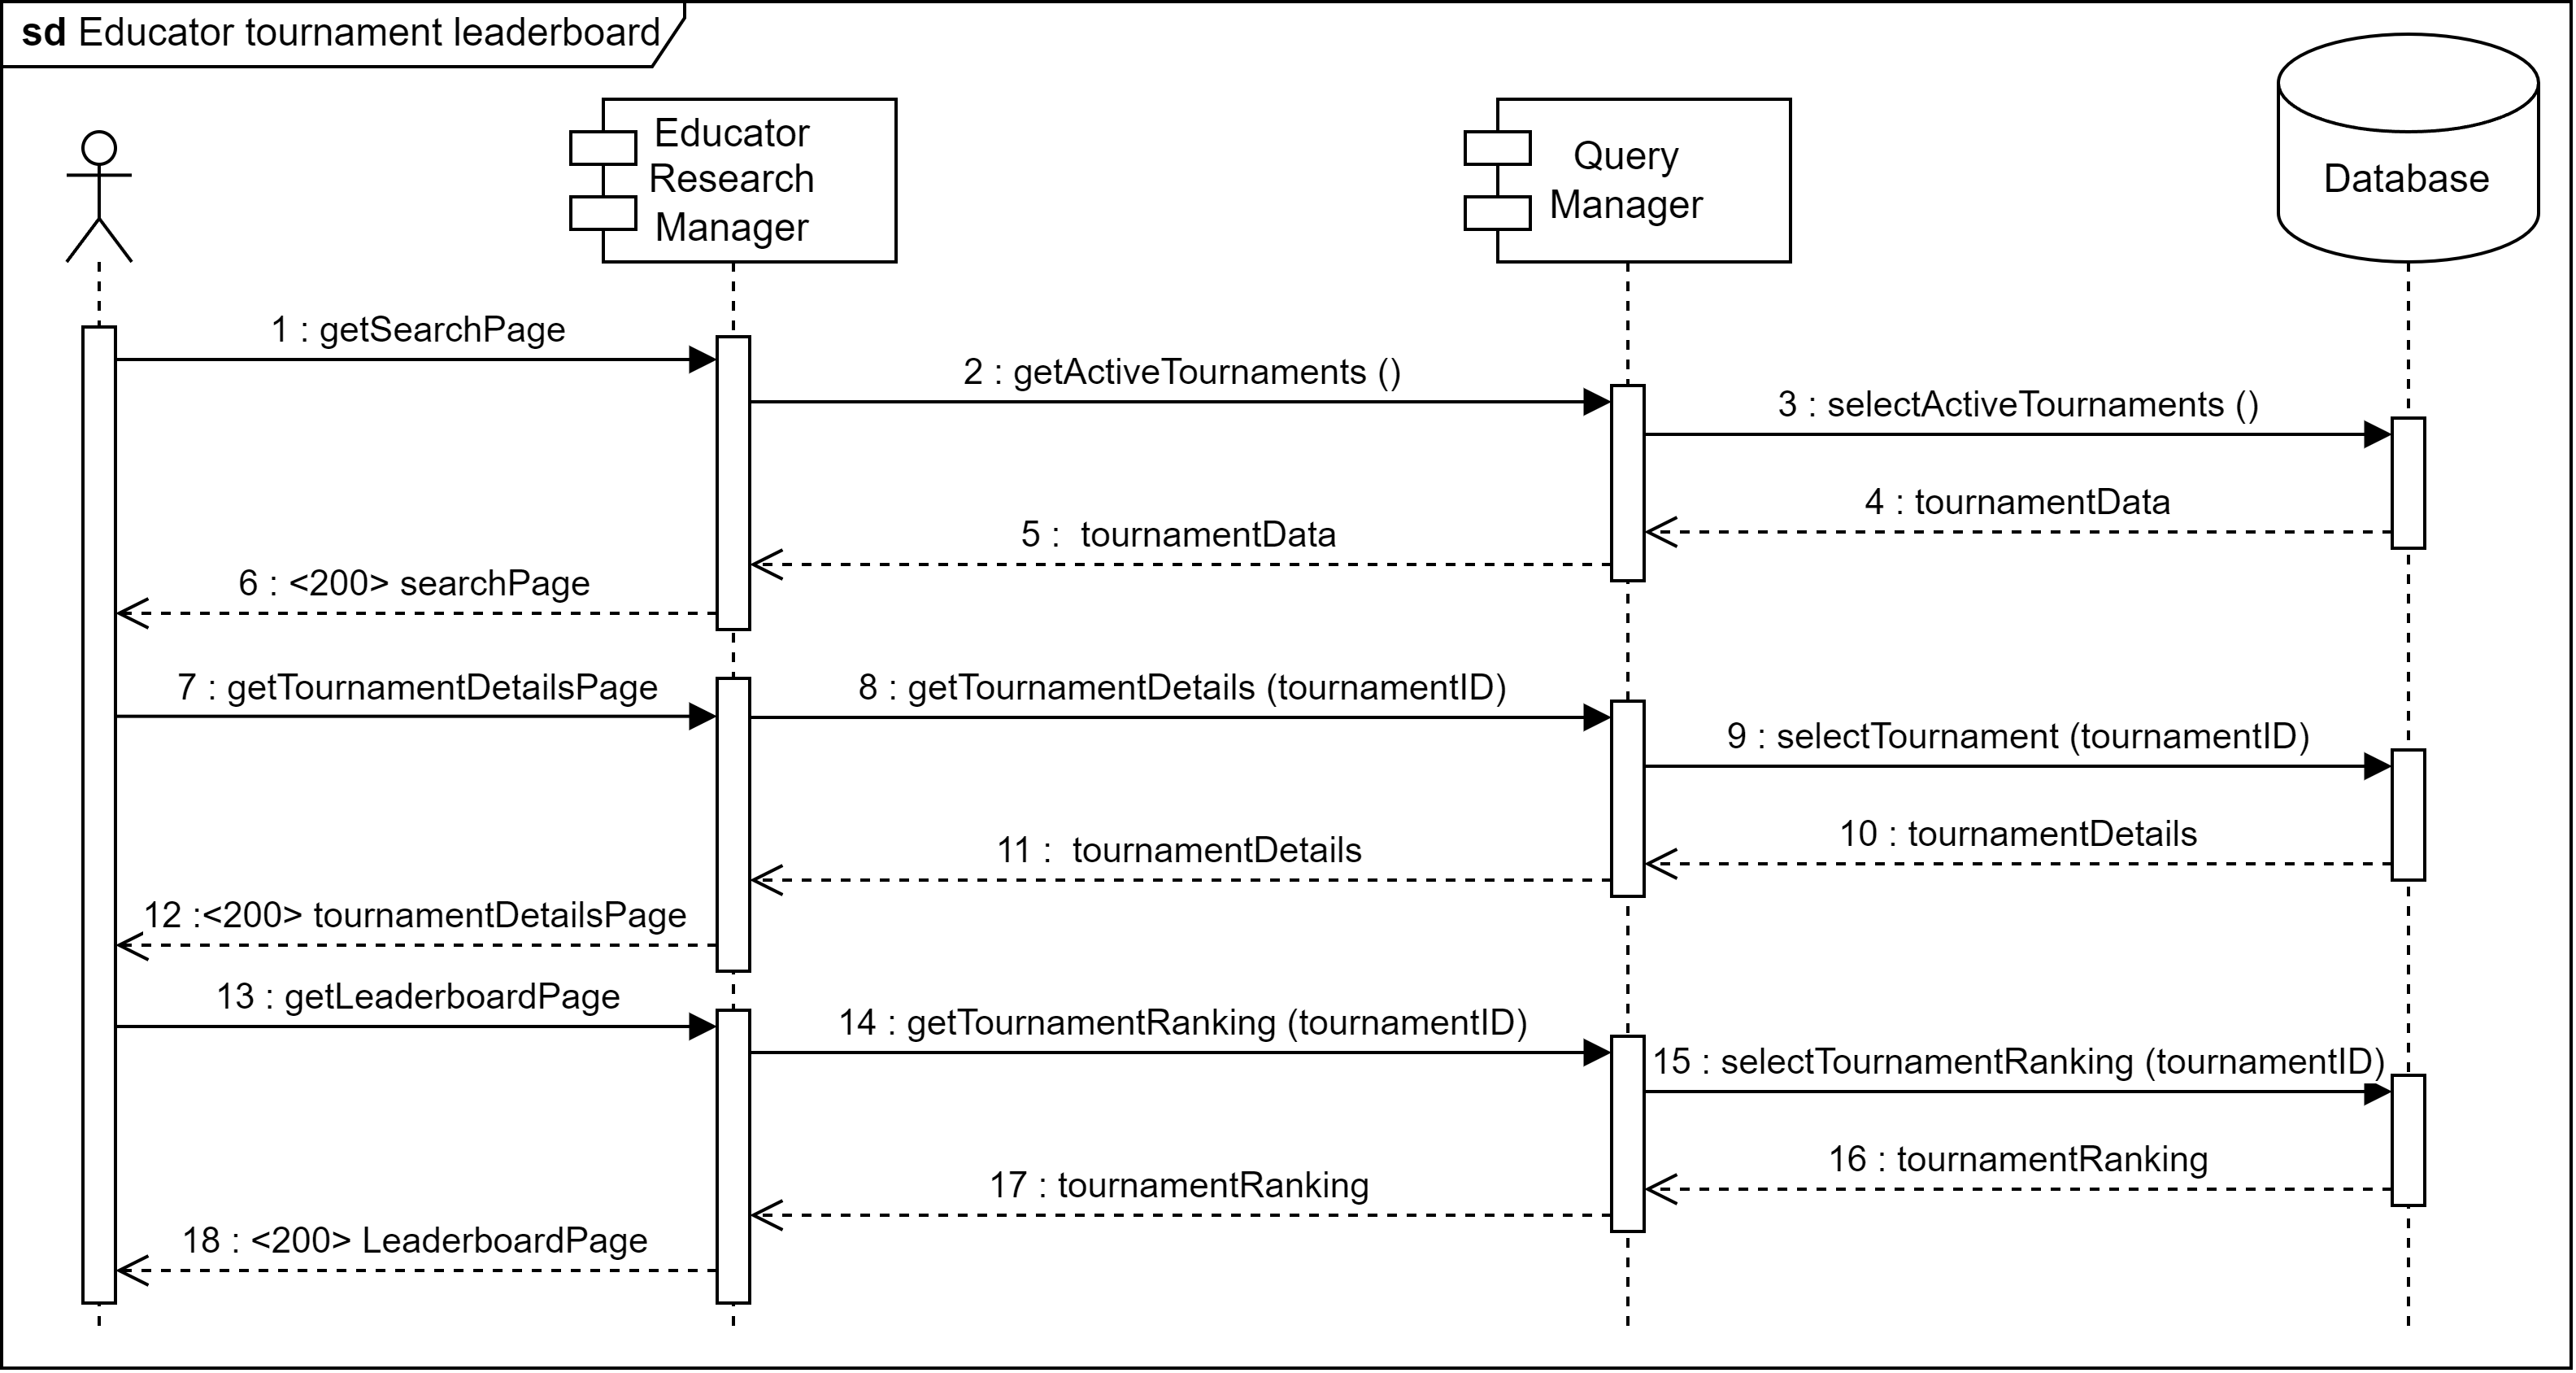
\includegraphics[width=1.0\linewidth]{images/etlrv.png}
    \end{figure}

    \paragraph*{User checks battle leaderboard}
    In this case the user is a registered student that wants to check the leaderboard of a tournament. 
    After accessing the search page and consequently the tournament details page the student can access the leaderboard page of the selected tournament. 
    After this he can click on the button linked to the desired battle within the selected tournament. 
    \begin{figure}[H]
        \centering
        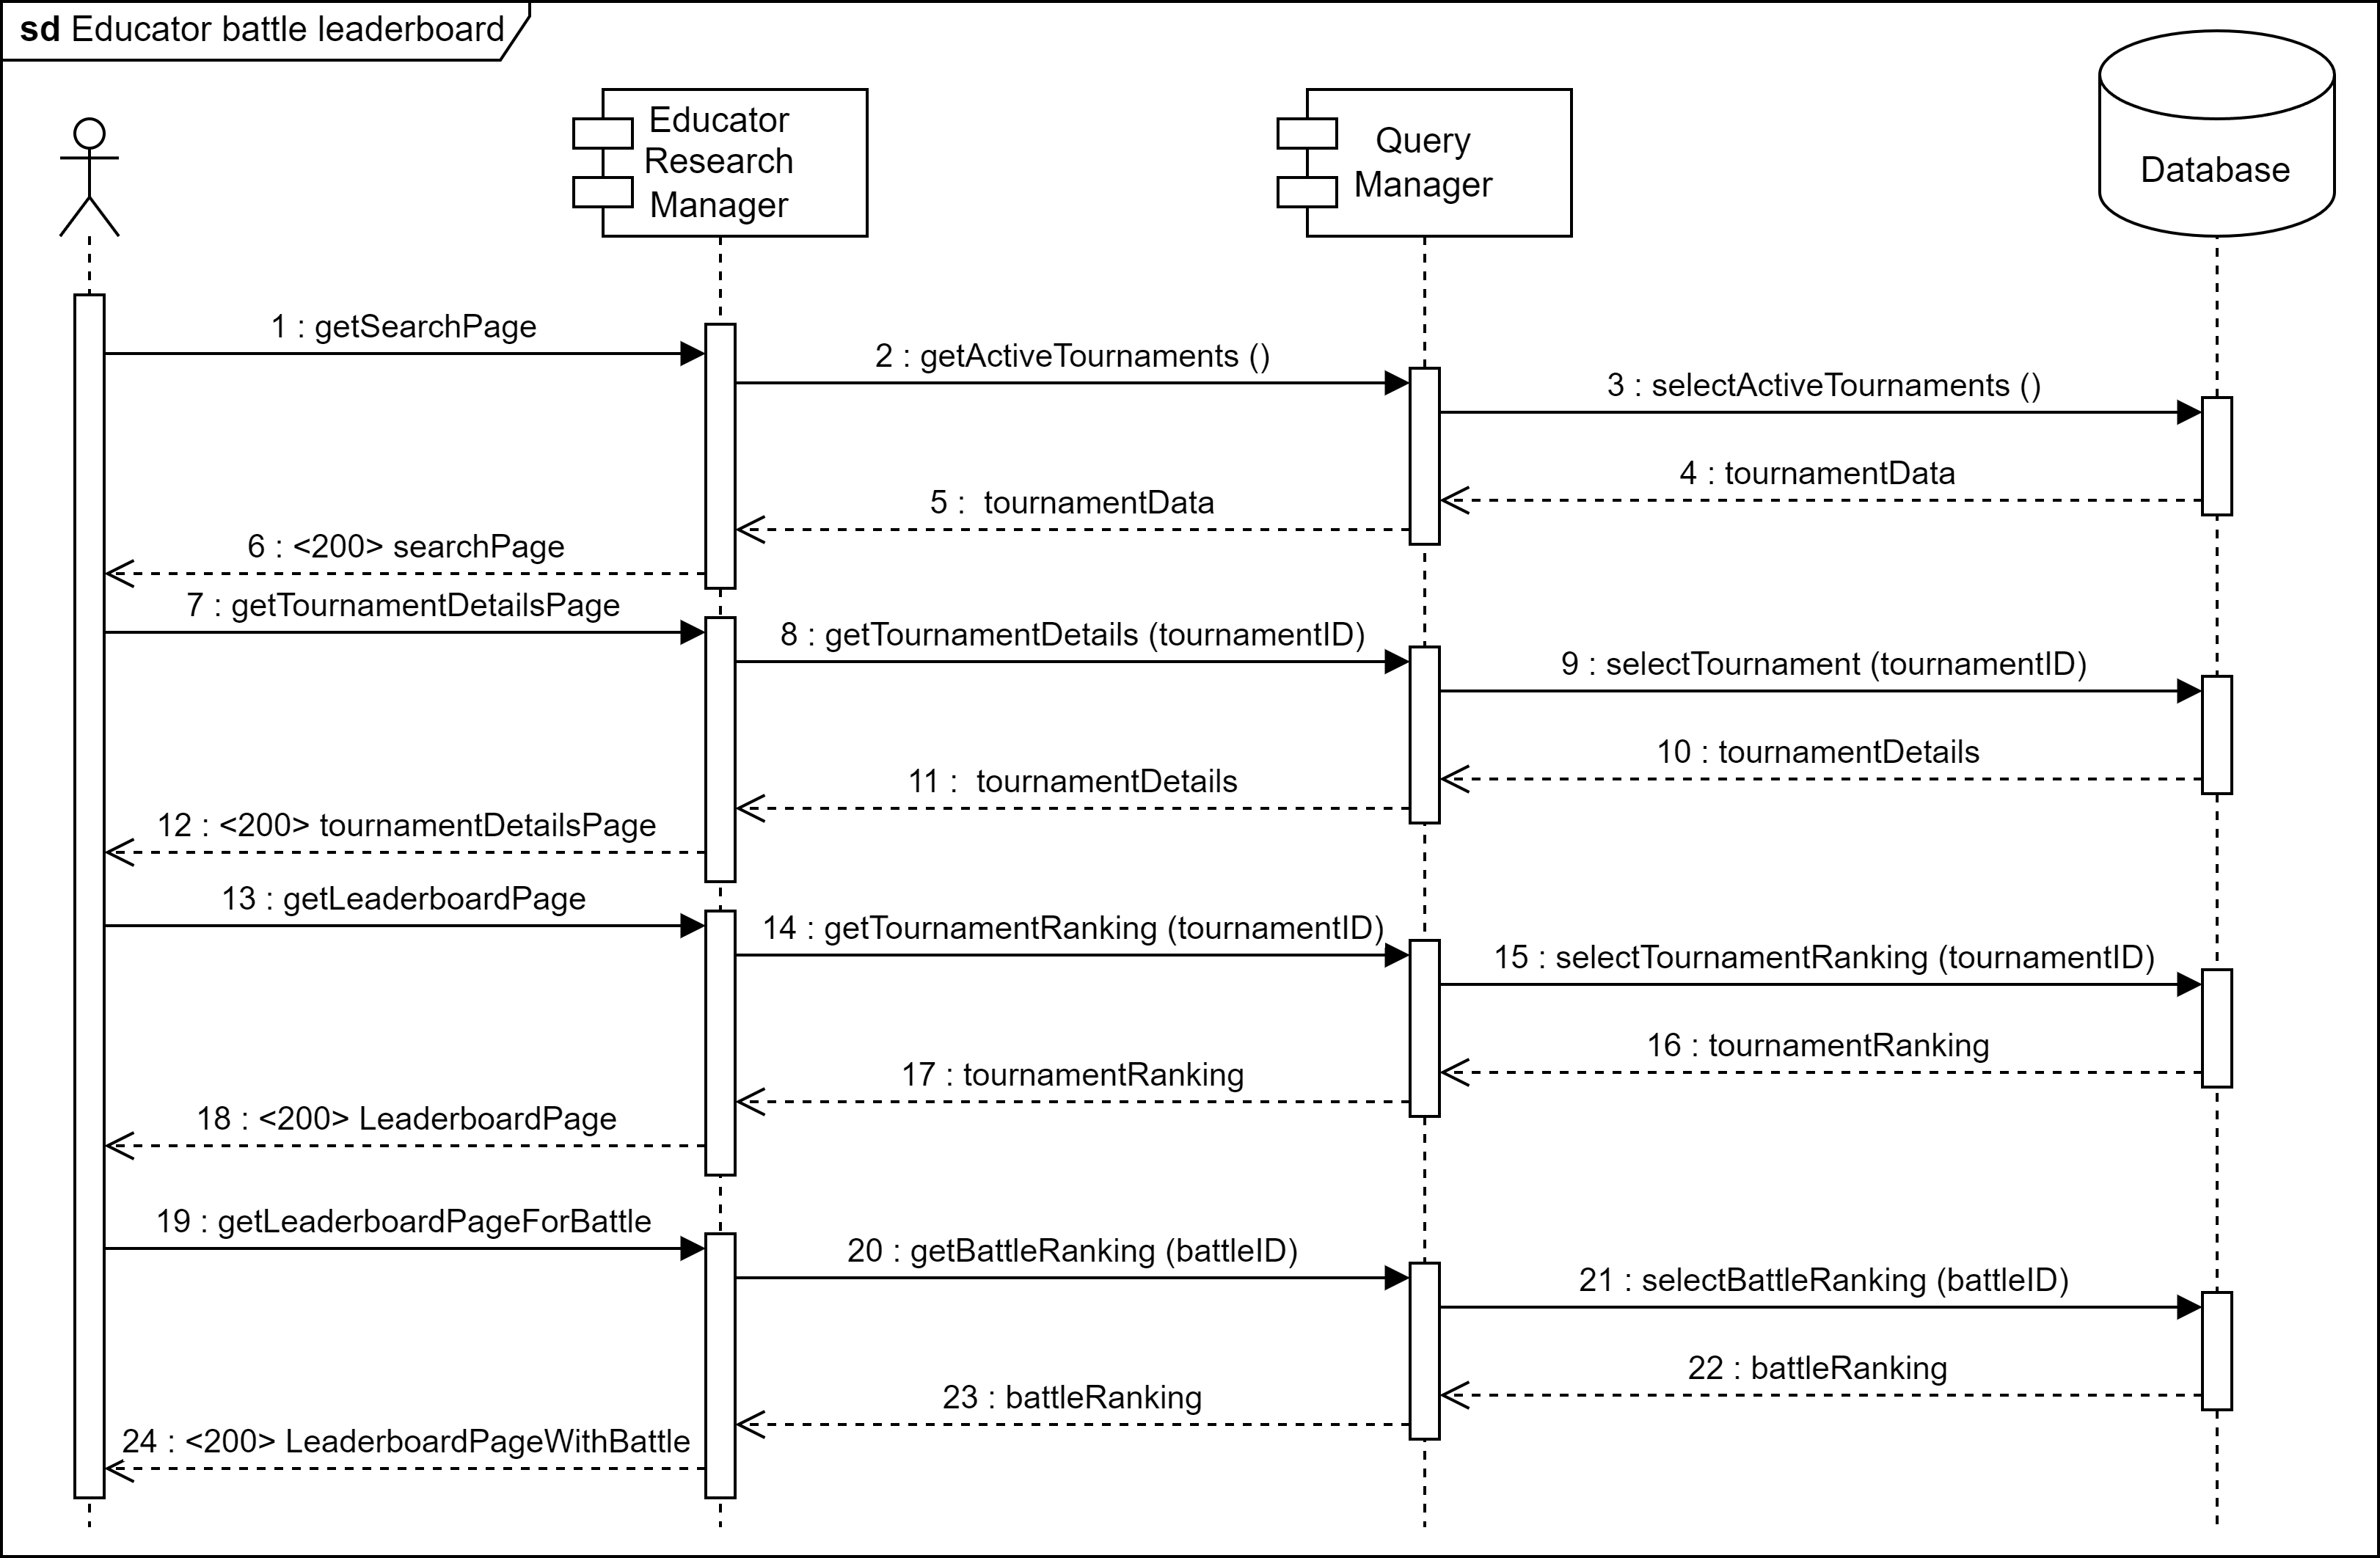
\includegraphics[width=1.0\linewidth]{images/eblrv.png}
    \end{figure}







































    \section{Component interfaces}
    \section{Selected architectural styles and patterns}
    \section{Other design decisions}

\newpage 

\chapter{User interface design}
    The user interface is the visual representation of how the application appears to the end user.
    It should be intuitive and straightforward, ensuring easy access to all features.
    Mockups were introduced in the RASD document, and now flowcharts for both students and educators will be presented.
    Flowcharts offer a concise and clear overview of the interactions and steps involved in utilizing the web app.
    \section{Flowchart for students UI}
    \begin{figure}[H]
        \centering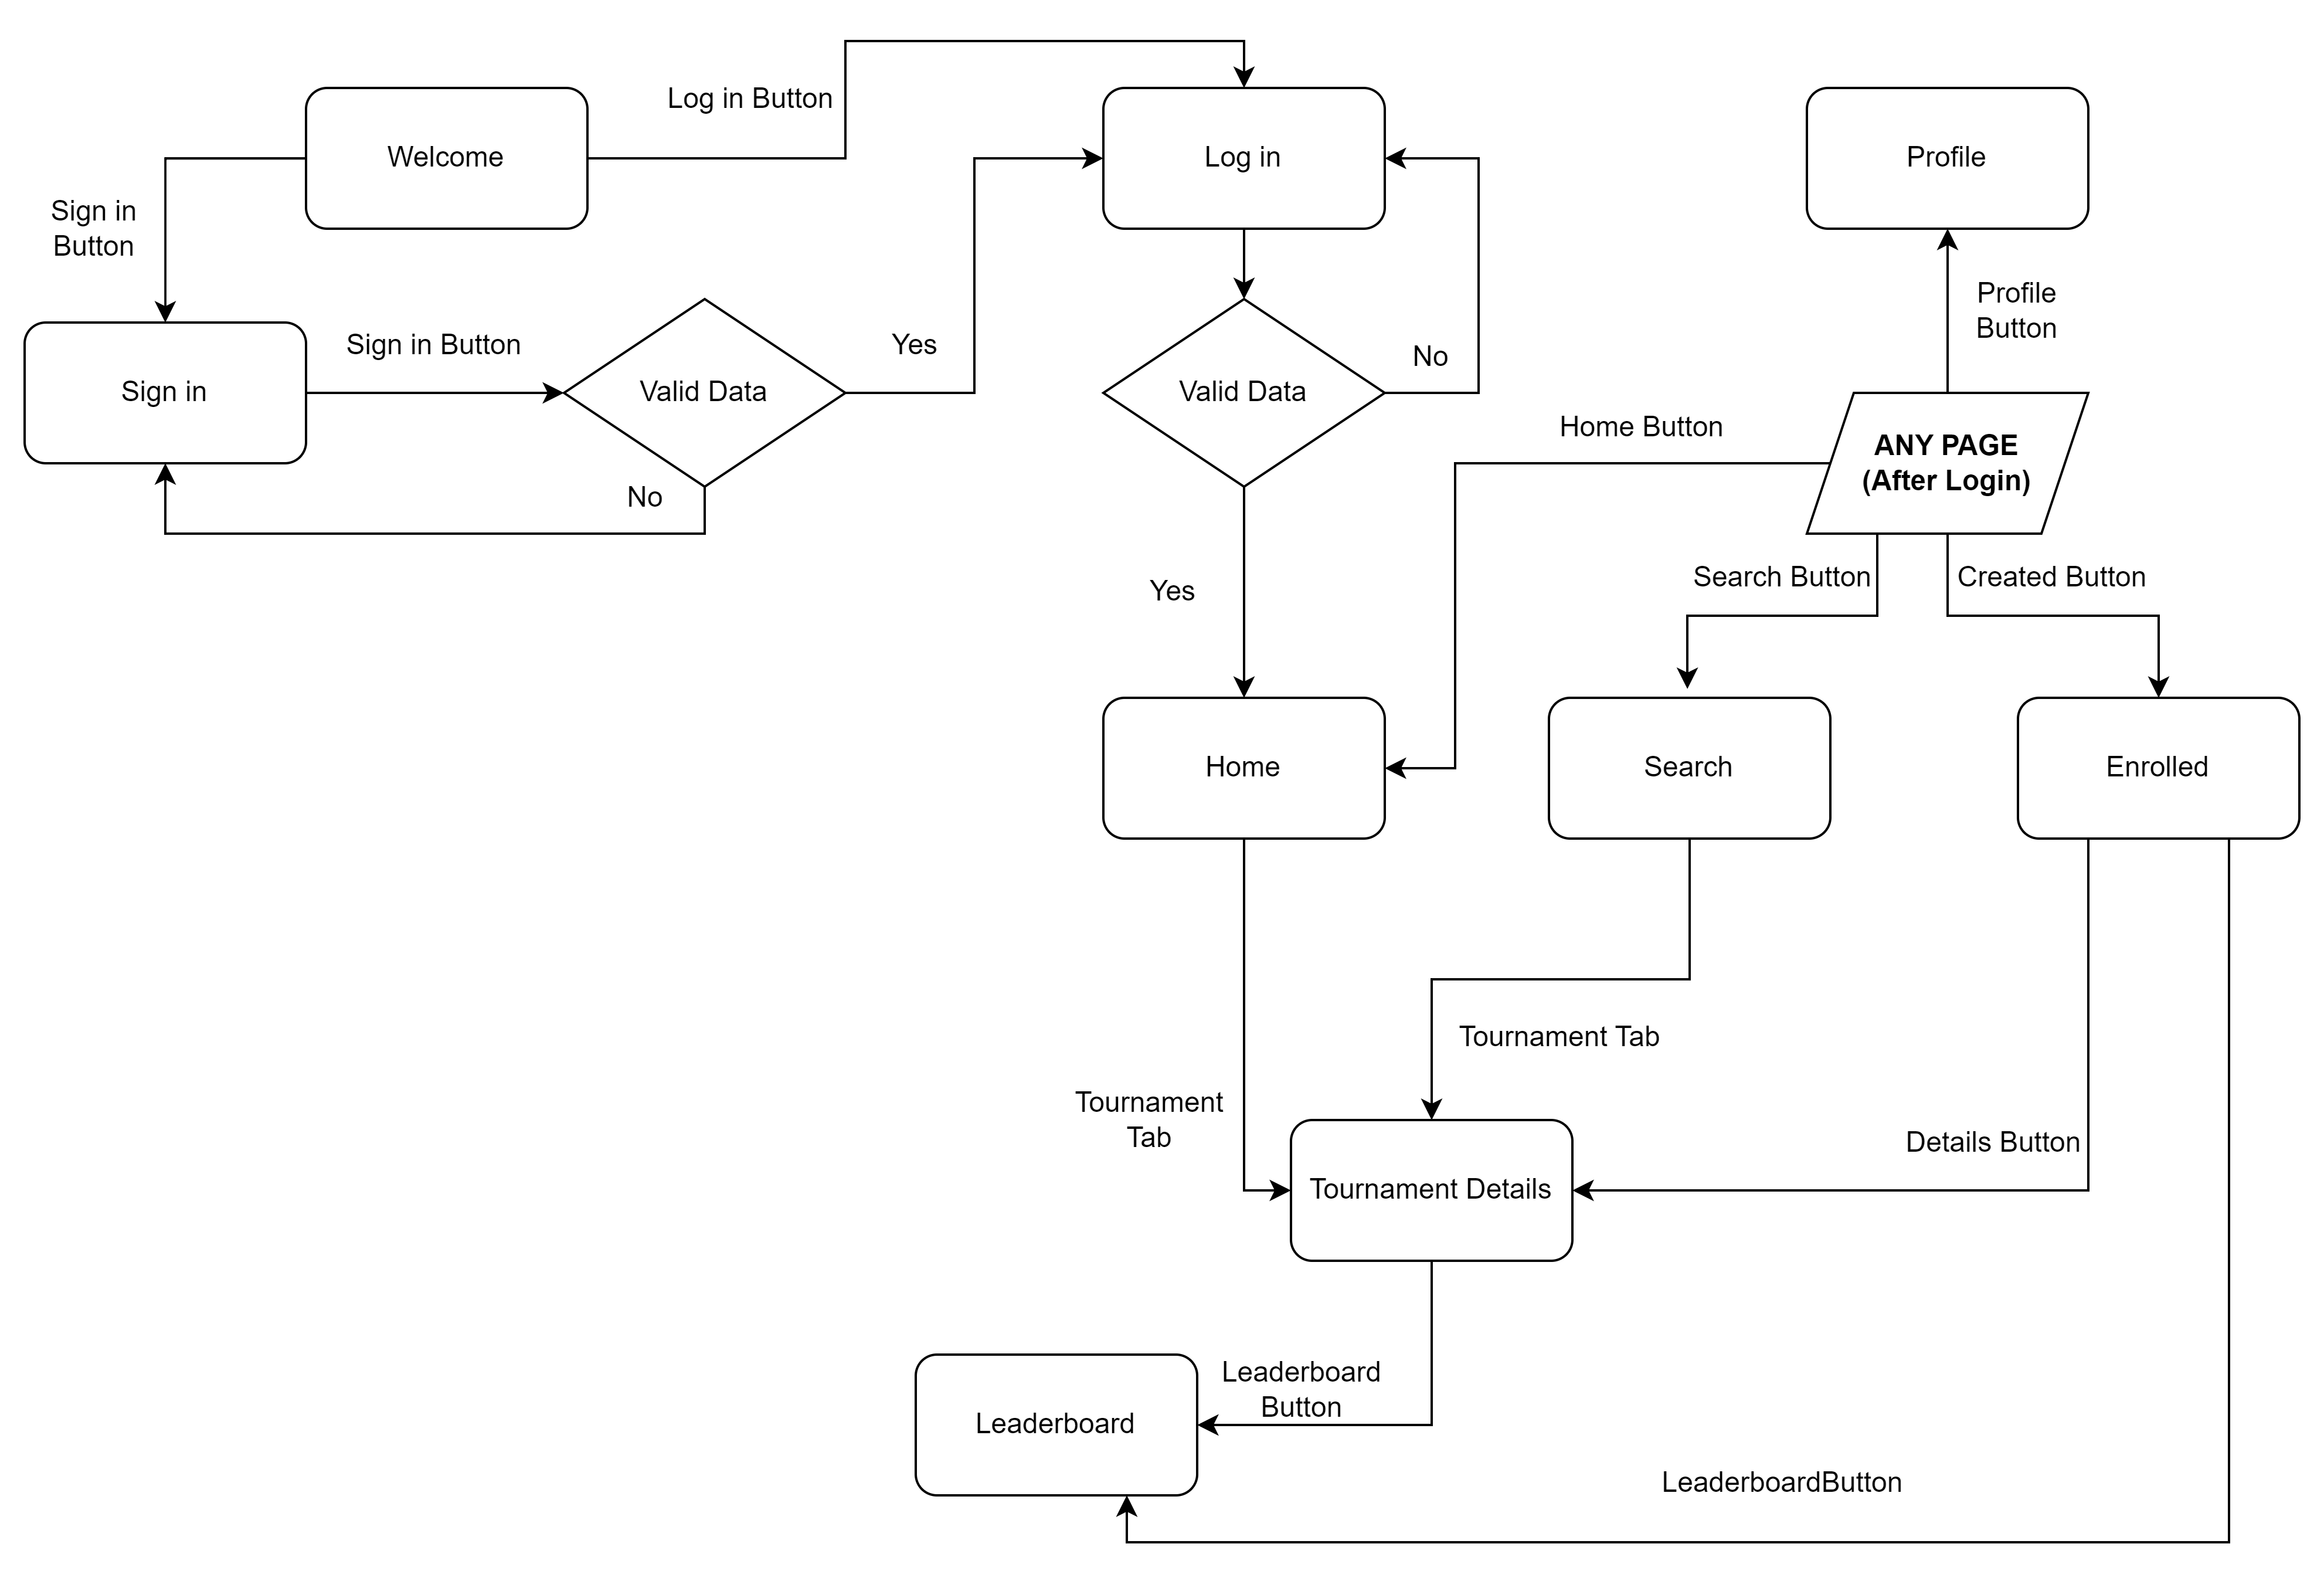
\includegraphics[width=0.9\linewidth]{images/students_UI.png}
    \end{figure}
    \section{Flowchart for educators UI}
    \begin{figure}[H]
        \centering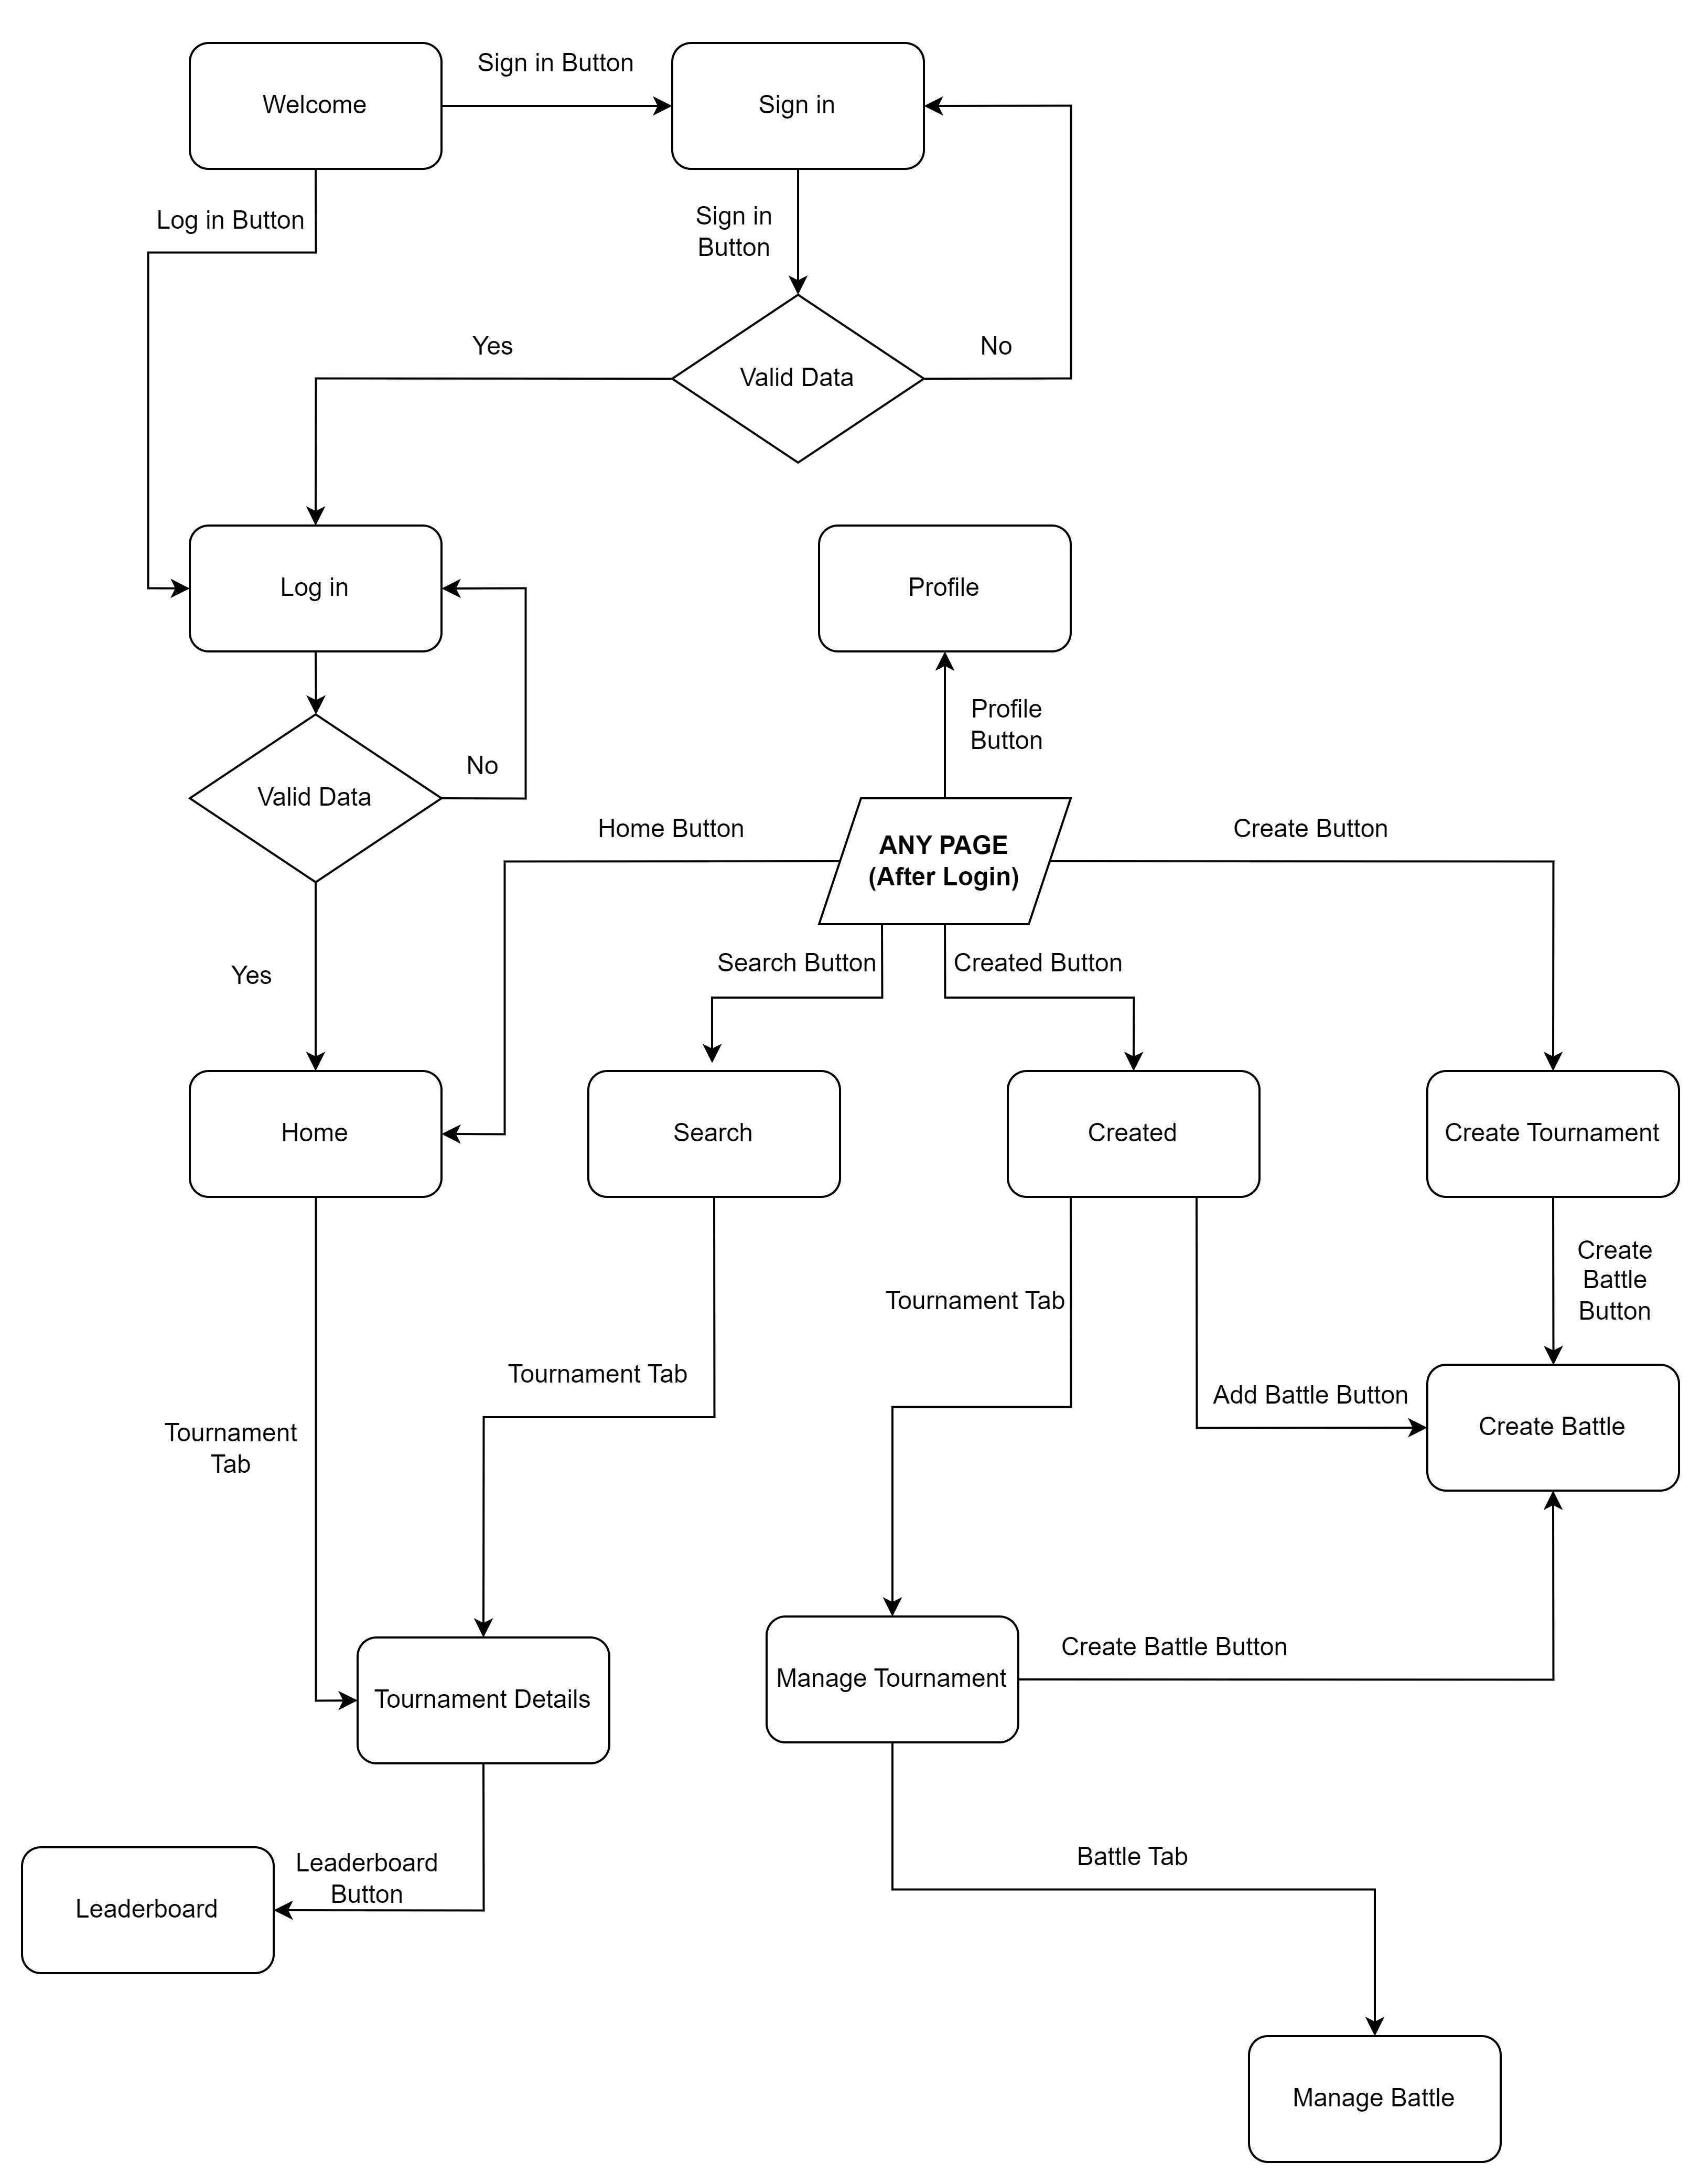
\includegraphics[width=0.9\linewidth]{images/educators_UI.png}
    \end{figure}

    \newpage 

\chapter{Requirements traceability}

\newpage 

\chapter{Implementation, integration and test plan}

\newpage 

\chapter{Effort spent}

\newpage 

\chapter{References}

\end{document}